% Output-side normalization in Muon-type optimizers (clean v2 draft: Methodology & Results first).
% Build: PATH=/opt/texlive/2026/bin/x86_64-linux:$PATH latexmk -pdf main.tex
\ifdefined\pdftexversion\pdfoutput=1\fi
\documentclass[11pt]{article}

\usepackage[utf8]{inputenc}
\usepackage[T1]{fontenc}
\usepackage{fullpage}
\usepackage{lmodern}
\usepackage{amsmath}
\usepackage{amssymb}
\usepackage{amsfonts}
\usepackage{amsthm}
\usepackage{graphicx}
\usepackage{booktabs}
\usepackage{longtable}
\usepackage{array}
\usepackage{multirow}
\usepackage{pifont}
\usepackage{placeins}
\usepackage{mdframed}
\usepackage{xurl}
\usepackage{nicefrac}
\usepackage{microtype}
\usepackage[table]{xcolor}
\usepackage[round]{natbib}
\PassOptionsToPackage{hyphens}{url}

\providecommand{\RNum}[1]{\uppercase\expandafter{\romannumeral #1\relax}}
\usepackage{caption}
\usepackage{hyperref}
\usepackage{cleveref}

\usepackage{tikz}
\usetikzlibrary{matrix, positioning}
\usepackage{pgfplots}
\pgfplotsset{compat=1.18}
\captionsetup[figure]{width=0.92\textwidth}
\usepackage{wrapfig}
\usepackage{needspace}
\usepackage{xcolor}
\usepackage{cancel}
\usepackage{acronym}

\renewcommand{\CancelColor}{\color{red}}

\def\stle{\overset{\mathrm{s.t.}}{\leq}}
\def\enc#1{\mathrm{enc}_{#1}}
\def\dec#1{\mathrm{dec}_{#1}}
\def\pre#1{\mathrm{pre}_{#1}}
\def\heaviside{\mathrm{Heav}}

\DeclareMathOperator*{\spn}{span}

\newcommand{\eqi}[1]{\overset{\text{(\romannumeral#1)}}{=}}
\newcommand{\brai}[1]{\text{(\romannumeral#1)}}
\newcommand{\braRNum}[1]{\text{(\RNum{#1})}}

\definecolor{mypink}{HTML}{FF1493}
\definecolor{darkred}{HTML}{BB253B}
\definecolor{lightgreen}{HTML}{90C0BF}
\newcommand{\highlight}[1]{{\textcolor{darkcyan}{#1}}}
\newcommand{\hermite}[1]{{he}_{#1}}
\def\addref{\textcolor{lightgreen}{\textbf{[Add Reference]}}}
\definecolor{darkcyan}{HTML}{0081B9}

\newmdenv[
  backgroundcolor=gray!10,
  skipabove=1em,
  skipbelow=1em,
  leftline=false,
  topline=false,
  bottomline=false,
  rightline=false,
  linecolor=gray!88,
  linewidth=4pt
]{githubquote}

\usepackage[most,skins,theorems]{tcolorbox}
\tcbset{
  aibox/.style={
    width=\linewidth,
    top=10pt,
    bottom=4pt,
    colback=blue!6!white,
    colframe=black,
    colbacktitle=black,
    enhanced,
    center,
    attach boxed title to top left={yshift=-0.1in,xshift=0.15in},
    boxed title style={boxrule=0pt,colframe=white,},
  }
}

\definecolor{rliableolive}{HTML}{BBCC33}
\definecolor{rliableblue}{HTML}{77AADD}
\definecolor{rliablered}{HTML}{EE8866}
\definecolor{LightCyan}{rgb}{0.88,1,1}
\definecolor{darkblue}{HTML}{2878D9}
\definecolor{navyblue}{HTML}{0000FF}

\newtcolorbox{AIbox}[2][]{aibox,title=#2,colback=rliableblue!10!white,#1}

\providecolor{yaleblue}{HTML}{00356B}
\colorlet{findingframe}{yaleblue}
\definecolor{findingaccent}{HTML}{D97757}
\colorlet{findingbg}{yaleblue!5!white}

\newtcolorbox[%
  auto counter,
  number within=section,
  crefname={finding}{findings},
  Crefname={Finding}{Findings},
]{finding}[1][]{%
  enhanced,
  breakable,
  before skip=10pt,
  after skip=10pt,
  colback=findingbg,
  colframe=findingframe,
  boxrule=0pt,
  arc=3pt,
  outer arc=3pt,
  left=12pt, right=12pt, top=8pt, bottom=10pt,
  before upper={%
    \noindent\textbf{Finding~\thetcbcounter\ifblank{#1}{}{. #1}.}\enspace
  },
}

\newenvironment{olivebox}{%
    \begin{tcolorbox}[colback=rliableolive!10!white,colframe=black,boxsep=3pt,top=4pt,bottom=4pt,left=3pt,right=3pt]
}{%
    \end{tcolorbox}
}

\newenvironment{lightbluebox}{%
    \begin{tcolorbox}[colback=rliableblue!15!white,colframe=gray!10!white,boxsep=3pt,top=4pt,bottom=4pt,left=3pt,right=3pt]
}{%
    \end{tcolorbox}
}
\newenvironment{bluebox}{%
    \begin{tcolorbox}[colback=navyblue!5!white,colframe=gray!20!white,boxsep=3pt,top=4pt,bottom=4pt,left=3pt,right=3pt]
}{%
    \end{tcolorbox}
}

\newenvironment{violetbox}{%
    \begin{tcolorbox}[colback=violet!10!white,colframe=black,boxsep=3pt,top=4pt,bottom=4pt,left=3pt,right=3pt]
}{%
    \end{tcolorbox}
}

\newenvironment{olivebox2}{%
    \begin{tcolorbox}[colback=rliableolive!10!white,colframe=gray!20!white,boxsep=3pt,top=4pt,bottom=4pt,left=3pt,right=3pt]
}{%
    \end{tcolorbox}
}

\usepackage{subcaption}

\usepackage{titlesec}
\usepackage{xcolor}
\definecolor{sectionblue}{HTML}{00356B}

\titleformat{\section}
  {\Large\bfseries\color{sectionblue}}{\thesection}{1em}{}
\titleformat{\subsection}
  {\large\bfseries\color{sectionblue}}{\thesubsection}{1em}{}
\titleformat{\subsubsection}
  {\normalsize\bfseries\color{sectionblue}}{\thesubsubsection}{1em}{}
\titleformat{\paragraph}[runin]
  {\normalfont\normalsize\bfseries\color{black}}{}{0pt}{}


% Clean full-page standard article typography and palette compatibility helpers.
\definecolor{pageink}{HTML}{1C2B33}
\definecolor{pagemuted}{HTML}{5F6B73}
\definecolor{pagelink}{HTML}{2E5AA8}
\definecolor{pagepanel}{HTML}{F1F4F7}
\definecolor{pageaccent}{HTML}{2E5AA8}
\definecolor{pagerule}{HTML}{D2D7DB}
\colorlet{sectionblue}{pageink}

\newcommand*{\pagesf}{\sffamily}
\newcommand*{\pagesfsb}{\sffamily\bfseries}

\titleformat{\section}{\normalfont\Large\bfseries\color{pageink}}{\thesection}{0.8em}{}
\titleformat{\subsection}{\normalfont\large\bfseries\color{pageink}}{\thesubsection}{0.75em}{}
\titleformat{\subsubsection}{\normalfont\normalsize\bfseries\color{pageink}}{\thesubsubsection}{0.75em}{}
\titleformat{\paragraph}[runin]{\normalfont\normalsize\bfseries\color{pageink}}{\theparagraph}{0.75em}{}
\titlespacing*{\paragraph}{0pt}{1.5ex plus 0.5ex minus 0.2ex}{0.75em}

\captionsetup{font=small, labelfont=bf, width=0.96\textwidth}
\hypersetup{
  colorlinks=true,
  linkcolor=pagelink,
  citecolor=pagelink,
  urlcolor=pagelink,
  hypertexnames=false
}

\urlstyle{tt}
\interfootnotelinepenalty=10000
\renewcommand{\topfraction}{0.88}
\renewcommand{\bottomfraction}{0.75}
\renewcommand{\textfraction}{0.10}
\renewcommand{\floatpagefraction}{0.75}
\newcommand{\todo}[1]{\textcolor{red}{[TODO: #1]}}

\graphicspath{{figs/}}
% Deterministic numeric macros generated from verified JSON summaries.
% Generated by scripts/integrate_sym_wave.py from results/summary.json. Do not edit.

% wave0/down_hybrid
\newcommand{\cselWaveZeroDownHybrid}{3.379440}
\newcommand{\cdselWaveZeroDownHybrid}{+0.002512}
\newcommand{\cdselfinalWaveZeroDownHybrid}{+0.001064}
\newcommand{\cdcfourWaveZeroDownHybrid}{+0.003605}
\newcommand{\cdcfourfinalWaveZeroDownHybrid}{+0.002358}
\newcommand{\cstepWaveZeroDownHybrid}{1.125}
\newcommand{\coverheadWaveZeroDownHybrid}{2.74}
\newcommand{\cetoeWaveZeroDownHybrid}{2.68}
\newcommand{\cmemWaveZeroDownHybrid}{19.23}
\newcommand{\cdtrainWaveZeroDownHybrid}{+0.003176}
\newcommand{\cdtrainseWaveZeroDownHybrid}{0.000047}
\newcommand{\cfbWaveZeroDownHybrid}{0}
% wave0/muon
\newcommand{\cselWaveZeroMuon}{3.382434}
\newcommand{\cdselWaveZeroMuon}{+0.005505}
\newcommand{\cdselfinalWaveZeroMuon}{+0.009484}
\newcommand{\cdcfourWaveZeroMuon}{+0.005345}
\newcommand{\cdcfourfinalWaveZeroMuon}{+0.009113}
\newcommand{\cstepWaveZeroMuon}{1.074}
\newcommand{\coverheadWaveZeroMuon}{-1.93}
\newcommand{\cetoeWaveZeroMuon}{-1.59}
\newcommand{\cmemWaveZeroMuon}{18.97}
\newcommand{\cdtrainWaveZeroMuon}{+0.006161}
\newcommand{\cdtrainseWaveZeroMuon}{0.000160}
\newcommand{\cfbWaveZeroMuon}{0}
% wave0/muont
\newcommand{\cselWaveZeroMuont}{3.376929}
\newcommand{\cdselWaveZeroMuont}{+0.000000}
\newcommand{\cdselfinalWaveZeroMuont}{+0.000000}
\newcommand{\cdcfourWaveZeroMuont}{+0.000000}
\newcommand{\cdcfourfinalWaveZeroMuont}{+0.000000}
\newcommand{\cstepWaveZeroMuont}{1.095}
\newcommand{\coverheadWaveZeroMuont}{0.00}
\newcommand{\cetoeWaveZeroMuont}{0.00}
\newcommand{\cmemWaveZeroMuont}{20.53}
\newcommand{\cdtrainWaveZeroMuont}{+0.000000}
\newcommand{\cdtrainseWaveZeroMuont}{0.000000}
\newcommand{\cfbWaveZeroMuont}{0}
% wave0/outer_left_down
\newcommand{\cselWaveZeroOuterLeftDown}{3.375559}
\newcommand{\cdselWaveZeroOuterLeftDown}{-0.001370}
\newcommand{\cdselfinalWaveZeroOuterLeftDown}{-0.001274}
\newcommand{\cdcfourWaveZeroOuterLeftDown}{-0.000782}
\newcommand{\cdcfourfinalWaveZeroOuterLeftDown}{-0.001343}
\newcommand{\cstepWaveZeroOuterLeftDown}{1.143}
\newcommand{\coverheadWaveZeroOuterLeftDown}{4.38}
\newcommand{\cetoeWaveZeroOuterLeftDown}{5.04}
\newcommand{\cmemWaveZeroOuterLeftDown}{20.57}
\newcommand{\cdtrainWaveZeroOuterLeftDown}{-0.001160}
\newcommand{\cdtrainseWaveZeroOuterLeftDown}{0.000040}
\newcommand{\cfbWaveZeroOuterLeftDown}{0}
% wave1/inner_outer_all
\newcommand{\cselWaveOneInnerOuterAll}{3.371147}
\newcommand{\cdselWaveOneInnerOuterAll}{-0.005782}
\newcommand{\cdselfinalWaveOneInnerOuterAll}{-0.006143}
\newcommand{\cdcfourWaveOneInnerOuterAll}{-0.006379}
\newcommand{\cdcfourfinalWaveOneInnerOuterAll}{-0.006899}
\newcommand{\cstepWaveOneInnerOuterAll}{1.524}
\newcommand{\coverheadWaveOneInnerOuterAll}{39.16}
\newcommand{\cetoeWaveOneInnerOuterAll}{44.20}
\newcommand{\cmemWaveOneInnerOuterAll}{24.20}
\newcommand{\cdtrainWaveOneInnerOuterAll}{-0.004975}
\newcommand{\cdtrainseWaveOneInnerOuterAll}{0.000040}
\newcommand{\cfbWaveOneInnerOuterAll}{31759}
% wave1/inner_outer_all_diag
\newcommand{\cselWaveOneInnerOuterAllDiag}{3.394940}
\newcommand{\cdselWaveOneInnerOuterAllDiag}{+0.018011}
\newcommand{\cdselfinalWaveOneInnerOuterAllDiag}{+0.007335}
\newcommand{\cdcfourWaveOneInnerOuterAllDiag}{+0.017686}
\newcommand{\cdcfourfinalWaveOneInnerOuterAllDiag}{+0.006499}
\newcommand{\cstepWaveOneInnerOuterAllDiag}{1.275}
\newcommand{\coverheadWaveOneInnerOuterAllDiag}{16.44}
\newcommand{\cetoeWaveOneInnerOuterAllDiag}{13.06}
\newcommand{\cmemWaveOneInnerOuterAllDiag}{21.37}
\newcommand{\cdtrainWaveOneInnerOuterAllDiag}{+0.013373}
\newcommand{\cdtrainseWaveOneInnerOuterAllDiag}{0.000306}
\newcommand{\cfbWaveOneInnerOuterAllDiag}{0}
% wave1/left_all
\newcommand{\cselWaveOneLeftAll}{3.385635}
\newcommand{\cdselWaveOneLeftAll}{+0.008707}
\newcommand{\cdselfinalWaveOneLeftAll}{+0.003252}
\newcommand{\cdcfourWaveOneLeftAll}{+0.010896}
\newcommand{\cdcfourfinalWaveOneLeftAll}{+0.005016}
\newcommand{\cstepWaveOneLeftAll}{1.463}
\newcommand{\coverheadWaveOneLeftAll}{33.56}
\newcommand{\cetoeWaveOneLeftAll}{41.00}
\newcommand{\cmemWaveOneLeftAll}{22.20}
\newcommand{\cdtrainWaveOneLeftAll}{+0.007866}
\newcommand{\cdtrainseWaveOneLeftAll}{0.000115}
\newcommand{\cfbWaveOneLeftAll}{33962}
% wave1/null_all
\newcommand{\cselWaveOneNullAll}{3.375643}
\newcommand{\cdselWaveOneNullAll}{-0.001286}
\newcommand{\cdselfinalWaveOneNullAll}{-0.001166}
\newcommand{\cdcfourWaveOneNullAll}{-0.002298}
\newcommand{\cdcfourfinalWaveOneNullAll}{-0.002158}
\newcommand{\cstepWaveOneNullAll}{1.510}
\newcommand{\coverheadWaveOneNullAll}{37.84}
\newcommand{\cetoeWaveOneNullAll}{44.95}
\newcommand{\cmemWaveOneNullAll}{24.20}
\newcommand{\cdtrainWaveOneNullAll}{-0.001362}
\newcommand{\cdtrainseWaveOneNullAll}{0.000040}
\newcommand{\cfbWaveOneNullAll}{32838}
% wave10/muont
\newcommand{\cselWaveOneZeroMuont}{3.375445}
\newcommand{\cdselWaveOneZeroMuont}{+0.000000}
\newcommand{\cdselfinalWaveOneZeroMuont}{+0.000000}
\newcommand{\cdcfourWaveOneZeroMuont}{+0.000000}
\newcommand{\cdcfourfinalWaveOneZeroMuont}{+0.000000}
\newcommand{\cstepWaveOneZeroMuont}{1.099}
\newcommand{\coverheadWaveOneZeroMuont}{0.00}
\newcommand{\cetoeWaveOneZeroMuont}{0.00}
\newcommand{\cmemWaveOneZeroMuont}{20.53}
\newcommand{\cdtrainWaveOneZeroMuont}{+0.000000}
\newcommand{\cdtrainseWaveOneZeroMuont}{0.000000}
\newcommand{\cfbWaveOneZeroMuont}{0}
% wave10/null_leftdiag_upstream_fused
\newcommand{\cselWaveOneZeroNullLeftdiagUpstreamFused}{3.373435}
\newcommand{\cdselWaveOneZeroNullLeftdiagUpstreamFused}{-0.002010}
\newcommand{\cdselfinalWaveOneZeroNullLeftdiagUpstreamFused}{-0.001404}
\newcommand{\cdcfourWaveOneZeroNullLeftdiagUpstreamFused}{-0.001222}
\newcommand{\cdcfourfinalWaveOneZeroNullLeftdiagUpstreamFused}{-0.001814}
\newcommand{\cstepWaveOneZeroNullLeftdiagUpstreamFused}{1.195}
\newcommand{\coverheadWaveOneZeroNullLeftdiagUpstreamFused}{8.71}
\newcommand{\cetoeWaveOneZeroNullLeftdiagUpstreamFused}{8.03}
\newcommand{\cmemWaveOneZeroNullLeftdiagUpstreamFused}{22.39}
\newcommand{\cdtrainWaveOneZeroNullLeftdiagUpstreamFused}{-0.001139}
\newcommand{\cdtrainseWaveOneZeroNullLeftdiagUpstreamFused}{0.000053}
\newcommand{\cfbWaveOneZeroNullLeftdiagUpstreamFused}{0}
% wave10/outer_leftdiag_fused
\newcommand{\cselWaveOneZeroOuterLeftdiagFused}{3.372193}
\newcommand{\cdselWaveOneZeroOuterLeftdiagFused}{-0.003252}
\newcommand{\cdselfinalWaveOneZeroOuterLeftdiagFused}{-0.003100}
\newcommand{\cdcfourWaveOneZeroOuterLeftdiagFused}{-0.001769}
\newcommand{\cdcfourfinalWaveOneZeroOuterLeftdiagFused}{-0.001800}
\newcommand{\cstepWaveOneZeroOuterLeftdiagFused}{1.195}
\newcommand{\coverheadWaveOneZeroOuterLeftdiagFused}{8.75}
\newcommand{\cetoeWaveOneZeroOuterLeftdiagFused}{8.40}
\newcommand{\cmemWaveOneZeroOuterLeftdiagFused}{22.39}
\newcommand{\cdtrainWaveOneZeroOuterLeftdiagFused}{-0.001656}
\newcommand{\cdtrainseWaveOneZeroOuterLeftdiagFused}{0.000055}
\newcommand{\cfbWaveOneZeroOuterLeftdiagFused}{0}
% wave10/outer_leftdiag_upstream_fused
\newcommand{\cselWaveOneZeroOuterLeftdiagUpstreamFused}{3.372991}
\newcommand{\cdselWaveOneZeroOuterLeftdiagUpstreamFused}{-0.002453}
\newcommand{\cdselfinalWaveOneZeroOuterLeftdiagUpstreamFused}{-0.001787}
\newcommand{\cdcfourWaveOneZeroOuterLeftdiagUpstreamFused}{-0.002597}
\newcommand{\cdcfourfinalWaveOneZeroOuterLeftdiagUpstreamFused}{-0.002743}
\newcommand{\cstepWaveOneZeroOuterLeftdiagUpstreamFused}{1.190}
\newcommand{\coverheadWaveOneZeroOuterLeftdiagUpstreamFused}{8.27}
\newcommand{\cetoeWaveOneZeroOuterLeftdiagUpstreamFused}{7.64}
\newcommand{\cmemWaveOneZeroOuterLeftdiagUpstreamFused}{22.39}
\newcommand{\cdtrainWaveOneZeroOuterLeftdiagUpstreamFused}{-0.001378}
\newcommand{\cdtrainseWaveOneZeroOuterLeftdiagUpstreamFused}{0.000046}
\newcommand{\cfbWaveOneZeroOuterLeftdiagUpstreamFused}{0}
% wave12/inner_outer_leftdiag
\newcommand{\cselWaveOneTwoInnerOuterLeftdiag}{3.524806}
\newcommand{\cdselWaveOneTwoInnerOuterLeftdiag}{+0.049294}
\newcommand{\cdselfinalWaveOneTwoInnerOuterLeftdiag}{+0.042416}
\newcommand{\cdcfourWaveOneTwoInnerOuterLeftdiag}{+0.049206}
\newcommand{\cdcfourfinalWaveOneTwoInnerOuterLeftdiag}{+0.042125}
\newcommand{\cstepWaveOneTwoInnerOuterLeftdiag}{1.256}
\newcommand{\coverheadWaveOneTwoInnerOuterLeftdiag}{14.22}
\newcommand{\cetoeWaveOneTwoInnerOuterLeftdiag}{14.76}
\newcommand{\cmemWaveOneTwoInnerOuterLeftdiag}{22.36}
\newcommand{\cdtrainWaveOneTwoInnerOuterLeftdiag}{+0.046858}
\newcommand{\cdtrainseWaveOneTwoInnerOuterLeftdiag}{0.000175}
\newcommand{\cfbWaveOneTwoInnerOuterLeftdiag}{0}
% wave12/muont
\newcommand{\cselWaveOneTwoMuont}{3.475512}
\newcommand{\cdselWaveOneTwoMuont}{+0.000000}
\newcommand{\cdselfinalWaveOneTwoMuont}{+0.000000}
\newcommand{\cdcfourWaveOneTwoMuont}{+0.000000}
\newcommand{\cdcfourfinalWaveOneTwoMuont}{+0.000000}
\newcommand{\cstepWaveOneTwoMuont}{1.100}
\newcommand{\coverheadWaveOneTwoMuont}{0.00}
\newcommand{\cetoeWaveOneTwoMuont}{0.00}
\newcommand{\cmemWaveOneTwoMuont}{20.53}
\newcommand{\cdtrainWaveOneTwoMuont}{+0.000000}
\newcommand{\cdtrainseWaveOneTwoMuont}{0.000000}
\newcommand{\cfbWaveOneTwoMuont}{0}
% wave12/outer_leftdiag
\newcommand{\cselWaveOneTwoOuterLeftdiag}{3.525768}
\newcommand{\cdselWaveOneTwoOuterLeftdiag}{+0.050256}
\newcommand{\cdselfinalWaveOneTwoOuterLeftdiag}{+0.031214}
\newcommand{\cdcfourWaveOneTwoOuterLeftdiag}{+0.048761}
\newcommand{\cdcfourfinalWaveOneTwoOuterLeftdiag}{+0.027780}
\newcommand{\cstepWaveOneTwoOuterLeftdiag}{1.212}
\newcommand{\coverheadWaveOneTwoOuterLeftdiag}{10.20}
\newcommand{\cetoeWaveOneTwoOuterLeftdiag}{9.87}
\newcommand{\cmemWaveOneTwoOuterLeftdiag}{22.36}
\newcommand{\cdtrainWaveOneTwoOuterLeftdiag}{+0.042437}
\newcommand{\cdtrainseWaveOneTwoOuterLeftdiag}{0.001121}
\newcommand{\cfbWaveOneTwoOuterLeftdiag}{0}
% wave12/outer_leftdiag_fused
\newcommand{\cselWaveOneTwoOuterLeftdiagFused}{3.472603}
\newcommand{\cdselWaveOneTwoOuterLeftdiagFused}{-0.002909}
\newcommand{\cdselfinalWaveOneTwoOuterLeftdiagFused}{-0.002349}
\newcommand{\cdcfourWaveOneTwoOuterLeftdiagFused}{-0.001806}
\newcommand{\cdcfourfinalWaveOneTwoOuterLeftdiagFused}{-0.002462}
\newcommand{\cstepWaveOneTwoOuterLeftdiagFused}{1.201}
\newcommand{\coverheadWaveOneTwoOuterLeftdiagFused}{9.19}
\newcommand{\cetoeWaveOneTwoOuterLeftdiagFused}{9.02}
\newcommand{\cmemWaveOneTwoOuterLeftdiagFused}{22.39}
\newcommand{\cdtrainWaveOneTwoOuterLeftdiagFused}{-0.002814}
\newcommand{\cdtrainseWaveOneTwoOuterLeftdiagFused}{0.000056}
\newcommand{\cfbWaveOneTwoOuterLeftdiagFused}{0}
% wave2/inner_outer_hidden
\newcommand{\cselWaveTwoInnerOuterHidden}{3.373861}
\newcommand{\cdselWaveTwoInnerOuterHidden}{-0.003068}
\newcommand{\cdselfinalWaveTwoInnerOuterHidden}{-0.003109}
\newcommand{\cdcfourWaveTwoInnerOuterHidden}{-0.002625}
\newcommand{\cdcfourfinalWaveTwoInnerOuterHidden}{-0.002685}
\newcommand{\cstepWaveTwoInnerOuterHidden}{1.293}
\newcommand{\coverheadWaveTwoInnerOuterHidden}{18.04}
\newcommand{\cetoeWaveTwoInnerOuterHidden}{16.77}
\newcommand{\cmemWaveTwoInnerOuterHidden}{21.51}
\newcommand{\cdtrainWaveTwoInnerOuterHidden}{-0.002132}
\newcommand{\cdtrainseWaveTwoInnerOuterHidden}{0.000039}
\newcommand{\cfbWaveTwoInnerOuterHidden}{20345}
% wave2/inner_outer_leftdiag
\newcommand{\cselWaveTwoInnerOuterLeftdiag}{3.372426}
\newcommand{\cdselWaveTwoInnerOuterLeftdiag}{-0.004503}
\newcommand{\cdselfinalWaveTwoInnerOuterLeftdiag}{-0.004131}
\newcommand{\cdcfourWaveTwoInnerOuterLeftdiag}{-0.003610}
\newcommand{\cdcfourfinalWaveTwoInnerOuterLeftdiag}{-0.003135}
\newcommand{\cstepWaveTwoInnerOuterLeftdiag}{1.209}
\newcommand{\coverheadWaveTwoInnerOuterLeftdiag}{10.40}
\newcommand{\cetoeWaveTwoInnerOuterLeftdiag}{8.17}
\newcommand{\cmemWaveTwoInnerOuterLeftdiag}{22.36}
\newcommand{\cdtrainWaveTwoInnerOuterLeftdiag}{-0.003688}
\newcommand{\cdtrainseWaveTwoInnerOuterLeftdiag}{0.000042}
\newcommand{\cfbWaveTwoInnerOuterLeftdiag}{0}
% wave2/inner_outer_mlpdiag
\newcommand{\cselWaveTwoInnerOuterMlpdiag}{3.370344}
\newcommand{\cdselWaveTwoInnerOuterMlpdiag}{-0.006584}
\newcommand{\cdselfinalWaveTwoInnerOuterMlpdiag}{-0.006888}
\newcommand{\cdcfourWaveTwoInnerOuterMlpdiag}{-0.006078}
\newcommand{\cdcfourfinalWaveTwoInnerOuterMlpdiag}{-0.006264}
\newcommand{\cstepWaveTwoInnerOuterMlpdiag}{1.336}
\newcommand{\coverheadWaveTwoInnerOuterMlpdiag}{21.95}
\newcommand{\cetoeWaveTwoInnerOuterMlpdiag}{19.34}
\newcommand{\cmemWaveTwoInnerOuterMlpdiag}{22.63}
\newcommand{\cdtrainWaveTwoInnerOuterMlpdiag}{-0.005065}
\newcommand{\cdtrainseWaveTwoInnerOuterMlpdiag}{0.000045}
\newcommand{\cfbWaveTwoInnerOuterMlpdiag}{19998}
% wave2/outer_left_all
\newcommand{\cselWaveTwoOuterLeftAll}{3.372952}
\newcommand{\cdselWaveTwoOuterLeftAll}{-0.003977}
\newcommand{\cdselfinalWaveTwoOuterLeftAll}{-0.004184}
\newcommand{\cdcfourWaveTwoOuterLeftAll}{-0.004774}
\newcommand{\cdcfourfinalWaveTwoOuterLeftAll}{-0.004068}
\newcommand{\cstepWaveTwoOuterLeftAll}{1.419}
\newcommand{\coverheadWaveTwoOuterLeftAll}{29.61}
\newcommand{\cetoeWaveTwoOuterLeftAll}{35.03}
\newcommand{\cmemWaveTwoOuterLeftAll}{24.20}
\newcommand{\cdtrainWaveTwoOuterLeftAll}{-0.003877}
\newcommand{\cdtrainseWaveTwoOuterLeftAll}{0.000041}
\newcommand{\cfbWaveTwoOuterLeftAll}{32410}
% wave3/inner_outer_all_lag
\newcommand{\cselWaveThreeInnerOuterAllLag}{3.371036}
\newcommand{\cdselWaveThreeInnerOuterAllLag}{-0.005893}
\newcommand{\cdselfinalWaveThreeInnerOuterAllLag}{-0.006211}
\newcommand{\cdcfourWaveThreeInnerOuterAllLag}{-0.005863}
\newcommand{\cdcfourfinalWaveThreeInnerOuterAllLag}{-0.005474}
\newcommand{\cstepWaveThreeInnerOuterAllLag}{1.375}
\newcommand{\coverheadWaveThreeInnerOuterAllLag}{25.59}
\newcommand{\cetoeWaveThreeInnerOuterAllLag}{31.29}
\newcommand{\cmemWaveThreeInnerOuterAllLag}{24.49}
\newcommand{\cdtrainWaveThreeInnerOuterAllLag}{-0.005729}
\newcommand{\cdtrainseWaveThreeInnerOuterAllLag}{0.000041}
\newcommand{\cfbWaveThreeInnerOuterAllLag}{32736}
% wave3/inner_outer_mlpdiag_seed1
\newcommand{\cselWaveThreeInnerOuterMlpdiagSeedOne}{3.323852}
\newcommand{\cdselWaveThreeInnerOuterMlpdiagSeedOne}{-0.004749}
\newcommand{\cdselfinalWaveThreeInnerOuterMlpdiagSeedOne}{-0.002534}
\newcommand{\cdcfourWaveThreeInnerOuterMlpdiagSeedOne}{-0.004153}
\newcommand{\cdcfourfinalWaveThreeInnerOuterMlpdiagSeedOne}{-0.003738}
\newcommand{\cstepWaveThreeInnerOuterMlpdiagSeedOne}{1.344}
\newcommand{\coverheadWaveThreeInnerOuterMlpdiagSeedOne}{22.45}
\newcommand{\cetoeWaveThreeInnerOuterMlpdiagSeedOne}{23.14}
\newcommand{\cmemWaveThreeInnerOuterMlpdiagSeedOne}{22.63}
\newcommand{\cdtrainWaveThreeInnerOuterMlpdiagSeedOne}{-0.003497}
\newcommand{\cdtrainseWaveThreeInnerOuterMlpdiagSeedOne}{0.000041}
\newcommand{\cfbWaveThreeInnerOuterMlpdiagSeedOne}{19755}
% wave3/muont_seed1
\newcommand{\cselWaveThreeMuontSeedOne}{3.328601}
\newcommand{\cdselWaveThreeMuontSeedOne}{+0.000000}
\newcommand{\cdselfinalWaveThreeMuontSeedOne}{+0.000000}
\newcommand{\cdcfourWaveThreeMuontSeedOne}{+0.000000}
\newcommand{\cdcfourfinalWaveThreeMuontSeedOne}{+0.000000}
\newcommand{\cstepWaveThreeMuontSeedOne}{1.097}
\newcommand{\coverheadWaveThreeMuontSeedOne}{0.00}
\newcommand{\cetoeWaveThreeMuontSeedOne}{0.00}
\newcommand{\cmemWaveThreeMuontSeedOne}{20.53}
\newcommand{\cdtrainWaveThreeMuontSeedOne}{+0.000000}
\newcommand{\cdtrainseWaveThreeMuontSeedOne}{0.000000}
\newcommand{\cfbWaveThreeMuontSeedOne}{0}
% wave3/null_mlpdiag
\newcommand{\cselWaveThreeNullMlpdiag}{3.376279}
\newcommand{\cdselWaveThreeNullMlpdiag}{-0.000649}
\newcommand{\cdselfinalWaveThreeNullMlpdiag}{-0.001332}
\newcommand{\cdcfourWaveThreeNullMlpdiag}{-0.002043}
\newcommand{\cdcfourfinalWaveThreeNullMlpdiag}{-0.002052}
\newcommand{\cstepWaveThreeNullMlpdiag}{1.332}
\newcommand{\coverheadWaveThreeNullMlpdiag}{21.63}
\newcommand{\cetoeWaveThreeNullMlpdiag}{20.36}
\newcommand{\cmemWaveThreeNullMlpdiag}{22.63}
\newcommand{\cdtrainWaveThreeNullMlpdiag}{-0.000688}
\newcommand{\cdtrainseWaveThreeNullMlpdiag}{0.000038}
\newcommand{\cfbWaveThreeNullMlpdiag}{21862}
% wave4-baseline/muont_seed2
\newcommand{\cselWaveFourBaselineMuontSeedTwo}{3.300743}
\newcommand{\cdselWaveFourBaselineMuontSeedTwo}{+0.000000}
\newcommand{\cdselfinalWaveFourBaselineMuontSeedTwo}{+0.000000}
\newcommand{\cdcfourWaveFourBaselineMuontSeedTwo}{+0.000000}
\newcommand{\cdcfourfinalWaveFourBaselineMuontSeedTwo}{+0.000000}
\newcommand{\cstepWaveFourBaselineMuontSeedTwo}{1.098}
\newcommand{\coverheadWaveFourBaselineMuontSeedTwo}{0.00}
\newcommand{\cetoeWaveFourBaselineMuontSeedTwo}{0.00}
\newcommand{\cmemWaveFourBaselineMuontSeedTwo}{20.53}
\newcommand{\cdtrainWaveFourBaselineMuontSeedTwo}{+0.000000}
\newcommand{\cdtrainseWaveFourBaselineMuontSeedTwo}{0.000000}
\newcommand{\cfbWaveFourBaselineMuontSeedTwo}{0}
% wave4/inner_outer_mlpdiag_1m
\newcommand{\cselWaveFourInnerOuterMlpdiagOnem}{3.389576}
\newcommand{\cdselWaveFourInnerOuterMlpdiagOnem}{-0.002029}
\newcommand{\cdselfinalWaveFourInnerOuterMlpdiagOnem}{-0.003630}
\newcommand{\cdcfourWaveFourInnerOuterMlpdiagOnem}{-0.003522}
\newcommand{\cdcfourfinalWaveFourInnerOuterMlpdiagOnem}{-0.003958}
\newcommand{\cstepWaveFourInnerOuterMlpdiagOnem}{2.386}
\newcommand{\coverheadWaveFourInnerOuterMlpdiagOnem}{14.06}
\newcommand{\cetoeWaveFourInnerOuterMlpdiagOnem}{14.53}
\newcommand{\cmemWaveFourInnerOuterMlpdiagOnem}{25.44}
\newcommand{\cdtrainWaveFourInnerOuterMlpdiagOnem}{-0.003121}
\newcommand{\cdtrainseWaveFourInnerOuterMlpdiagOnem}{0.000064}
\newcommand{\cfbWaveFourInnerOuterMlpdiagOnem}{11245}
% wave4/inner_outer_mlpdiag_lag
\newcommand{\cselWaveFourInnerOuterMlpdiagLag}{3.371246}
\newcommand{\cdselWaveFourInnerOuterMlpdiagLag}{-0.005683}
\newcommand{\cdselfinalWaveFourInnerOuterMlpdiagLag}{-0.006555}
\newcommand{\cdcfourWaveFourInnerOuterMlpdiagLag}{-0.004987}
\newcommand{\cdcfourfinalWaveFourInnerOuterMlpdiagLag}{-0.004751}
\newcommand{\cstepWaveFourInnerOuterMlpdiagLag}{1.292}
\newcommand{\coverheadWaveFourInnerOuterMlpdiagLag}{17.95}
\newcommand{\cetoeWaveFourInnerOuterMlpdiagLag}{16.73}
\newcommand{\cmemWaveFourInnerOuterMlpdiagLag}{22.68}
\newcommand{\cdtrainWaveFourInnerOuterMlpdiagLag}{-0.004952}
\newcommand{\cdtrainseWaveFourInnerOuterMlpdiagLag}{0.000041}
\newcommand{\cfbWaveFourInnerOuterMlpdiagLag}{19651}
% wave4/inner_outer_mlpdiag_seed2
\newcommand{\cselWaveFourInnerOuterMlpdiagSeedTwo}{3.297046}
\newcommand{\cdselWaveFourInnerOuterMlpdiagSeedTwo}{-0.003697}
\newcommand{\cdselfinalWaveFourInnerOuterMlpdiagSeedTwo}{-0.003609}
\newcommand{\cdcfourWaveFourInnerOuterMlpdiagSeedTwo}{-0.003967}
\newcommand{\cdcfourfinalWaveFourInnerOuterMlpdiagSeedTwo}{-0.003651}
\newcommand{\cstepWaveFourInnerOuterMlpdiagSeedTwo}{1.351}
\newcommand{\coverheadWaveFourInnerOuterMlpdiagSeedTwo}{23.08}
\newcommand{\cetoeWaveFourInnerOuterMlpdiagSeedTwo}{22.53}
\newcommand{\cmemWaveFourInnerOuterMlpdiagSeedTwo}{22.63}
\newcommand{\cdtrainWaveFourInnerOuterMlpdiagSeedTwo}{-0.003453}
\newcommand{\cdtrainseWaveFourInnerOuterMlpdiagSeedTwo}{0.000045}
\newcommand{\cfbWaveFourInnerOuterMlpdiagSeedTwo}{19512}
% wave4/muont_1m
\newcommand{\cselWaveFourMuontOnem}{3.391605}
\newcommand{\cdselWaveFourMuontOnem}{+0.000000}
\newcommand{\cdselfinalWaveFourMuontOnem}{+0.000000}
\newcommand{\cdcfourWaveFourMuontOnem}{+0.000000}
\newcommand{\cdcfourfinalWaveFourMuontOnem}{+0.000000}
\newcommand{\cstepWaveFourMuontOnem}{2.092}
\newcommand{\coverheadWaveFourMuontOnem}{0.00}
\newcommand{\cetoeWaveFourMuontOnem}{0.00}
\newcommand{\cmemWaveFourMuontOnem}{21.51}
\newcommand{\cdtrainWaveFourMuontOnem}{+0.000000}
\newcommand{\cdtrainseWaveFourMuontOnem}{0.000000}
\newcommand{\cfbWaveFourMuontOnem}{0}
% wave7/inner_outer_leftdiag
\newcommand{\cselWaveSevenInnerOuterLeftdiag}{3.372553}
\newcommand{\cdselWaveSevenInnerOuterLeftdiag}{-0.002892}
\newcommand{\cdselfinalWaveSevenInnerOuterLeftdiag}{-0.002514}
\newcommand{\cdcfourWaveSevenInnerOuterLeftdiag}{-0.003238}
\newcommand{\cdcfourfinalWaveSevenInnerOuterLeftdiag}{-0.003831}
\newcommand{\cstepWaveSevenInnerOuterLeftdiag}{1.212}
\newcommand{\coverheadWaveSevenInnerOuterLeftdiag}{10.24}
\newcommand{\cetoeWaveSevenInnerOuterLeftdiag}{9.98}
\newcommand{\cmemWaveSevenInnerOuterLeftdiag}{22.36}
\newcommand{\cdtrainWaveSevenInnerOuterLeftdiag}{-0.001862}
\newcommand{\cdtrainseWaveSevenInnerOuterLeftdiag}{0.000053}
\newcommand{\cfbWaveSevenInnerOuterLeftdiag}{0}
% wave7/muont
\newcommand{\cselWaveSevenMuont}{3.375445}
\newcommand{\cdselWaveSevenMuont}{+0.000000}
\newcommand{\cdselfinalWaveSevenMuont}{+0.000000}
\newcommand{\cdcfourWaveSevenMuont}{+0.000000}
\newcommand{\cdcfourfinalWaveSevenMuont}{+0.000000}
\newcommand{\cstepWaveSevenMuont}{1.099}
\newcommand{\coverheadWaveSevenMuont}{0.00}
\newcommand{\cetoeWaveSevenMuont}{0.00}
\newcommand{\cmemWaveSevenMuont}{20.53}
\newcommand{\cdtrainWaveSevenMuont}{+0.000000}
\newcommand{\cdtrainseWaveSevenMuont}{0.000000}
\newcommand{\cfbWaveSevenMuont}{0}
% wave7/outer_leftdiag
\newcommand{\cselWaveSevenOuterLeftdiag}{3.373427}
\newcommand{\cdselWaveSevenOuterLeftdiag}{-0.002018}
\newcommand{\cdselfinalWaveSevenOuterLeftdiag}{-0.000858}
\newcommand{\cdcfourWaveSevenOuterLeftdiag}{-0.002605}
\newcommand{\cdcfourfinalWaveSevenOuterLeftdiag}{-0.002679}
\newcommand{\cstepWaveSevenOuterLeftdiag}{1.213}
\newcommand{\coverheadWaveSevenOuterLeftdiag}{10.36}
\newcommand{\cetoeWaveSevenOuterLeftdiag}{9.77}
\newcommand{\cmemWaveSevenOuterLeftdiag}{22.36}
\newcommand{\cdtrainWaveSevenOuterLeftdiag}{-0.001552}
\newcommand{\cdtrainseWaveSevenOuterLeftdiag}{0.000063}
\newcommand{\cfbWaveSevenOuterLeftdiag}{0}
% wave7/outer_leftdiag_fused
\newcommand{\cselWaveSevenOuterLeftdiagFused}{3.374167}
\newcommand{\cdselWaveSevenOuterLeftdiagFused}{-0.001277}
\newcommand{\cdselfinalWaveSevenOuterLeftdiagFused}{-0.000115}
\newcommand{\cdcfourWaveSevenOuterLeftdiagFused}{-0.002226}
\newcommand{\cdcfourfinalWaveSevenOuterLeftdiagFused}{-0.002188}
\newcommand{\cstepWaveSevenOuterLeftdiagFused}{1.203}
\newcommand{\coverheadWaveSevenOuterLeftdiagFused}{9.45}
\newcommand{\cetoeWaveSevenOuterLeftdiagFused}{8.86}
\newcommand{\cmemWaveSevenOuterLeftdiagFused}{22.39}
\newcommand{\cdtrainWaveSevenOuterLeftdiagFused}{-0.001518}
\newcommand{\cdtrainseWaveSevenOuterLeftdiagFused}{0.000056}
\newcommand{\cfbWaveSevenOuterLeftdiagFused}{0}
% wave_sym_fastlag/muont
\newcommand{\cselWaveSymFastlagMuont}{3.376348}
\newcommand{\cdselWaveSymFastlagMuont}{+0.000000}
\newcommand{\cdselfinalWaveSymFastlagMuont}{+0.000000}
\newcommand{\cdcfourWaveSymFastlagMuont}{+0.000000}
\newcommand{\cdcfourfinalWaveSymFastlagMuont}{+0.000000}
\newcommand{\cstepWaveSymFastlagMuont}{1.099}
\newcommand{\coverheadWaveSymFastlagMuont}{0.00}
\newcommand{\cetoeWaveSymFastlagMuont}{0.00}
\newcommand{\cmemWaveSymFastlagMuont}{20.53}
\newcommand{\cdtrainWaveSymFastlagMuont}{+0.000000}
\newcommand{\cdtrainseWaveSymFastlagMuont}{0.000000}
\newcommand{\cfbWaveSymFastlagMuont}{0}
% wave_sym_fastlag/inner_outer_sym_mlpdiag
\newcommand{\cselWaveSymFastlagInnerOuterSymMlpdiag}{3.373833}
\newcommand{\cdselWaveSymFastlagInnerOuterSymMlpdiag}{-0.002515}
\newcommand{\cdselfinalWaveSymFastlagInnerOuterSymMlpdiag}{-0.002994}
\newcommand{\cdcfourWaveSymFastlagInnerOuterSymMlpdiag}{-0.002028}
\newcommand{\cdcfourfinalWaveSymFastlagInnerOuterSymMlpdiag}{-0.002876}
\newcommand{\cstepWaveSymFastlagInnerOuterSymMlpdiag}{1.234}
\newcommand{\coverheadWaveSymFastlagInnerOuterSymMlpdiag}{12.36}
\newcommand{\cetoeWaveSymFastlagInnerOuterSymMlpdiag}{11.93}
\newcommand{\cmemWaveSymFastlagInnerOuterSymMlpdiag}{20.73}
\newcommand{\cdtrainWaveSymFastlagInnerOuterSymMlpdiag}{-0.001261}
\newcommand{\cdtrainseWaveSymFastlagInnerOuterSymMlpdiag}{0.000045}
\newcommand{\cfbWaveSymFastlagInnerOuterSymMlpdiag}{22860}
% wave_sym_fastlag/inner_outer_sym_mlpdiag_lag
\newcommand{\cselWaveSymFastlagInnerOuterSymMlpdiagLag}{3.375221}
\newcommand{\cdselWaveSymFastlagInnerOuterSymMlpdiagLag}{-0.001127}
\newcommand{\cdselfinalWaveSymFastlagInnerOuterSymMlpdiagLag}{-0.002456}
\newcommand{\cdcfourWaveSymFastlagInnerOuterSymMlpdiagLag}{-0.001603}
\newcommand{\cdcfourfinalWaveSymFastlagInnerOuterSymMlpdiagLag}{-0.002905}
\newcommand{\cstepWaveSymFastlagInnerOuterSymMlpdiagLag}{1.141}
\newcommand{\coverheadWaveSymFastlagInnerOuterSymMlpdiagLag}{3.84}
\newcommand{\cetoeWaveSymFastlagInnerOuterSymMlpdiagLag}{4.89}
\newcommand{\cmemWaveSymFastlagInnerOuterSymMlpdiagLag}{20.81}
\newcommand{\cdtrainWaveSymFastlagInnerOuterSymMlpdiagLag}{-0.001478}
\newcommand{\cdtrainseWaveSymFastlagInnerOuterSymMlpdiagLag}{0.000040}
\newcommand{\cfbWaveSymFastlagInnerOuterSymMlpdiagLag}{21762}
% wave_sym_fastlag/inner_outer_mlpdiag_lag
\newcommand{\cselWaveSymFastlagInnerOuterMlpdiagLag}{3.371610}
\newcommand{\cdselWaveSymFastlagInnerOuterMlpdiagLag}{-0.004737}
\newcommand{\cdselfinalWaveSymFastlagInnerOuterMlpdiagLag}{-0.004291}
\newcommand{\cdcfourWaveSymFastlagInnerOuterMlpdiagLag}{-0.002621}
\newcommand{\cdcfourfinalWaveSymFastlagInnerOuterMlpdiagLag}{-0.002074}
\newcommand{\cstepWaveSymFastlagInnerOuterMlpdiagLag}{1.162}
\newcommand{\coverheadWaveSymFastlagInnerOuterMlpdiagLag}{5.75}
\newcommand{\cetoeWaveSymFastlagInnerOuterMlpdiagLag}{6.94}
\newcommand{\cmemWaveSymFastlagInnerOuterMlpdiagLag}{21.59}
\newcommand{\cdtrainWaveSymFastlagInnerOuterMlpdiagLag}{-0.001996}
\newcommand{\cdtrainseWaveSymFastlagInnerOuterMlpdiagLag}{0.000040}
\newcommand{\cfbWaveSymFastlagInnerOuterMlpdiagLag}{19991}

% Generated by scripts/analyze_lr.py from the screening trials. Do not edit.

\newcommand{\lrMuontBest}{4.251046}
\newcommand{\lrMuontBestLR}{0.06400}
\newcommand{\lrMuontBase}{4.422130}
\newcommand{\lrMuontGainFromTuning}{0.171084}
\newcommand{\lrBestMuont}{4.251046}
\newcommand{\lrBestLRMuont}{0.06400}
\newcommand{\lrMarginMuont}{0.000000}
\newcommand{\lrBaseMuont}{4.422130}
\newcommand{\lrSameLRMarginMuont}{0.000000}
\newcommand{\lrBestInnerOuterLeftdiag}{4.231413}
\newcommand{\lrBestLRInnerOuterLeftdiag}{0.09051}
\newcommand{\lrMarginInnerOuterLeftdiag}{-0.019633}
\newcommand{\lrBaseInnerOuterLeftdiag}{4.431168}
\newcommand{\lrSameLRMarginInnerOuterLeftdiag}{0.009038}
\newcommand{\lrBestOuterLeftdiag}{4.236747}
\newcommand{\lrBestLROuterLeftdiag}{0.09051}
\newcommand{\lrMarginOuterLeftdiag}{-0.014299}
\newcommand{\lrBaseOuterLeftdiag}{4.441723}
\newcommand{\lrSameLRMarginOuterLeftdiag}{0.019593}
\newcommand{\lrBestOuterLeftdiagFused}{4.241099}
\newcommand{\lrBestLROuterLeftdiagFused}{0.06400}
\newcommand{\lrMarginOuterLeftdiagFused}{-0.009946}
\newcommand{\lrBaseOuterLeftdiagFused}{4.441234}
\newcommand{\lrSameLRMarginOuterLeftdiagFused}{0.019104}

% Generated by scripts/derive.py. Do not edit.

\newcommand{\mlpdiagsel}{-0.0066}
\newcommand{\mlpdiagselmag}{0.0066}
\newcommand{\leftallsel}{+0.0087}
\newcommand{\nullallsel}{-0.001286}
\newcommand{\nullmlpsel}{-0.000649}
\newcommand{\nullmlpselFour}{-0.0006}
\newcommand{\nullsharedense}{22}
\newcommand{\nullsharemlpcfour}{34}
\newcommand{\transferWorst}{0.050}
\newcommand{\lrHeadroom}{0.171}
\newcommand{\lrHeadroomRatio}{26}
\newcommand{\shortBaseInnerOuterLeftdiag}{+0.009038}
\newcommand{\shortBaseOuterLeftdiag}{+0.019593}
\newcommand{\shortBaseOuterLeftdiagFused}{+0.019104}
\newcommand{\waveTwelveMuontSelDiff}{+0.1001}
\newcommand{\waveTwelveMuontSelDiffMag}{0.100}
\newcommand{\waveTwelveMuontCfourDiff}{+0.0402}
\newcommand{\symWaveExactSteps}{22}
\newcommand{\symWaveMuontInFb}{13}
\newcommand{\waveZeroMuontInFb}{19}
\newcommand{\symWaveMuontVsWaveZeroSel}{-0.0006}
\newcommand{\symWaveMuontVsWaveZeroSelSix}{-0.000581}
\newcommand{\symWaveMuontVsWaveZeroCfourFinal}{-0.0016}
\newcommand{\symWaveMuontCfourFinalAbs}{3.4511}
\newcommand{\waveZeroMuonCfourFinalAbs}{3.4618}
\newcommand{\fastMlpLagSelSame}{-0.0047}
\newcommand{\fastMlpLagSelWaveZero}{-0.0053}
\newcommand{\fastMlpLagSelFinalSame}{-0.0043}
\newcommand{\fastMlpLagSelFinalWaveZero}{-0.0055}
\newcommand{\fastMlpLagCfourSame}{-0.0026}
\newcommand{\fastMlpLagCfourWaveZero}{-0.0040}
\newcommand{\fastMlpLagCfourFinalSame}{-0.0021}
\newcommand{\fastMlpLagCfourFinalAbs}{3.4491}
\newcommand{\fastMlpLagSelLateAbs}{3.3716}
\newcommand{\fastMlpLagWinOneSame}{-0.0110}
\newcommand{\fastMlpLagWinOneSeSame}{0.0009}
\newcommand{\fastMlpLagWinFiveSame}{-0.0020}
\newcommand{\fastMlpLagInFb}{67}
\newcommand{\symMlpSelSame}{-0.0025}
\newcommand{\symMlpSelWaveZero}{-0.0031}
\newcommand{\symMlpSelFinalSame}{-0.0030}
\newcommand{\symMlpCfourSame}{-0.0020}
\newcommand{\symMlpCfourWaveZero}{-0.0034}
\newcommand{\symMlpCfourFinalSame}{-0.0029}
\newcommand{\symMlpCfourFinalAbs}{3.4483}
\newcommand{\symMlpWinOneSame}{+0.0065}
\newcommand{\symMlpWinOneSeSame}{0.0019}
\newcommand{\symMlpWinFiveSame}{-0.0013}
\newcommand{\symMlpInFb}{0}
\newcommand{\symMlpLagSelSame}{-0.0011}
\newcommand{\symMlpLagSelWaveZero}{-0.0017}
\newcommand{\symMlpLagSelFinalSame}{-0.0025}
\newcommand{\symMlpLagCfourSame}{-0.0016}
\newcommand{\symMlpLagCfourWaveZero}{-0.0030}
\newcommand{\symMlpLagCfourFinalSame}{-0.0029}
\newcommand{\symMlpLagCfourFinalAbs}{3.4482}
\newcommand{\symMlpLagSelLateAbs}{3.3752}
\newcommand{\symMlpLagWinOneSame}{+0.0071}
\newcommand{\symMlpLagWinOneSeSame}{0.0014}
\newcommand{\symMlpLagWinFiveSame}{-0.0015}
\newcommand{\symMlpLagInFb}{4}
\newcommand{\symLagVsMlpLagWinOne}{+0.0181}
\newcommand{\symLagVsMlpLagWinOneSe}{0.0024}
\newcommand{\symLagVsMlpLagWinTwo}{+0.0041}
\newcommand{\symLagVsMlpLagWinThree}{+0.0026}
\newcommand{\symLagVsMlpLagWinFour}{+0.0010}
\newcommand{\symLagVsMlpLagWinFive}{+0.0005}
\newcommand{\symLagVsMlpLagSelLate}{+0.0036}
\newcommand{\symLagVsMlpLagSelLateMag}{0.0036}
\newcommand{\symLagVsMlpLagSelFinalMag}{0.0018}
\newcommand{\symLagVsMlpLagCfourFinal}{-0.0008}

% Generated by scripts/integrate_sym_wave.py. Do not edit.
\newcommand{\nRunDirs}{45}
\newcommand{\nDistinctRuns}{37}
\newcommand{\nDuplicateGroups}{5}
\newcommand{\nDuplicateDirs}{13}
\newcommand{\nOptimizerArms}{19}

% Generated by scripts/analyze_mechanism.py (wave1/null_all motivating audit). Do not edit.

\newcommand{\motInAttnErankMedPct}{17.9}
\newcommand{\motInAttnErankMeanPct}{15.5}
\newcommand{\motInAttnDiagCvMed}{0.84}
\newcommand{\motInAttnDiagCvMean}{1.37}
\newcommand{\motInAttnDiagMaxMean}{25.8}
\newcommand{\motInAttnDiagMaxMed}{11.3}
\newcommand{\motInAttnDiagMaxPeak}{145}
\newcommand{\motInAttnCorrRmsMed}{0.2031}
\newcommand{\motInAttnCorrRmsMean}{0.2251}
\newcommand{\motInAttnBulkCorrRmsMean}{0.2071}
\newcommand{\motInAttnDiagEMedPct}{3.5}
\newcommand{\motInAttnDiagEMeanPct}{8.3}
\newcommand{\motInAttnDiagAnisoMedPct}{1.0}
\newcommand{\motInAttnDiagAnisoMeanPct}{6.4}
\newcommand{\motInAttnBulkDiagAnisoMedPct}{1.6}
\newcommand{\motInAttnBulkDiagAnisoMeanPct}{7.3}
\newcommand{\motInAttnExpVarLMedPct}{10.6}
\newcommand{\motInAttnExpVarLMeanPct}{13.8}
\newcommand{\motInAttnBulkExpVarLMedPct}{12.0}
\newcommand{\motInAttnBulkExpVarLMeanPct}{14.8}
\newcommand{\motInAttnExpVarLhatMedPct}{-5.8}
\newcommand{\motInAttnExpVarLhatMeanPct}{-5.9}
\newcommand{\motInAttnCosLMed}{0.9290}
\newcommand{\motInAttnCosLMean}{0.9173}
\newcommand{\motInAttnRelErrLMed}{0.500}
\newcommand{\motInAttnRelErrLMean}{0.531}
\newcommand{\motInAttnDropErrLMed}{0.522}
\newcommand{\motInAttnDropErrLMean}{0.570}
\newcommand{\motInAttnTrajDiagAnisoMedPct}{1.1}
\newcommand{\motInAttnTrajDiagAnisoMeanPct}{5.6}
\newcommand{\motInAttnTrajExpVarLMedPct}{8.9}
\newcommand{\motInAttnTrajExpVarLMeanPct}{11.5}
\newcommand{\motInAttnTrajCorrRmsMed}{0.1810}
\newcommand{\motInAttnTrajErankMedPct}{20.9}
\newcommand{\motInAttnTrajDiagCvMean}{1.16}
\newcommand{\motInAttnDriftTopSixteenMean}{0.021}
\newcommand{\motInAttnDriftTopSixteenMed}{0.017}
\newcommand{\motInAttnDriftTopThirtyTwoMean}{0.031}
\newcommand{\motInAttnDriftTopThirtyTwoMed}{0.026}
\newcommand{\motInAttnCachedEstOverTolMed}{0.03}
\newcommand{\motInAttnShortDriftTopSixteen}{0.0006}
\newcommand{\motInOErankMedPct}{20.8}
\newcommand{\motInOErankMeanPct}{20.1}
\newcommand{\motInODiagCvMed}{0.75}
\newcommand{\motInODiagCvMean}{0.79}
\newcommand{\motInODiagMaxMean}{5.4}
\newcommand{\motInODiagMaxMed}{4.7}
\newcommand{\motInODiagMaxPeak}{13}
\newcommand{\motInOCorrRmsMed}{0.2120}
\newcommand{\motInOCorrRmsMean}{0.2313}
\newcommand{\motInOBulkCorrRmsMean}{0.2046}
\newcommand{\motInODiagEMedPct}{5.3}
\newcommand{\motInODiagEMeanPct}{7.6}
\newcommand{\motInODiagAnisoMedPct}{1.8}
\newcommand{\motInODiagAnisoMeanPct}{3.2}
\newcommand{\motInOBulkDiagAnisoMedPct}{2.5}
\newcommand{\motInOBulkDiagAnisoMeanPct}{3.5}
\newcommand{\motInOExpVarLMedPct}{22.5}
\newcommand{\motInOExpVarLMeanPct}{21.8}
\newcommand{\motInOBulkExpVarLMedPct}{23.2}
\newcommand{\motInOBulkExpVarLMeanPct}{22.6}
\newcommand{\motInOExpVarLhatMedPct}{23.9}
\newcommand{\motInOExpVarLhatMeanPct}{22.9}
\newcommand{\motInOCosLMed}{0.8643}
\newcommand{\motInOCosLMean}{0.8596}
\newcommand{\motInORelErrLMed}{0.659}
\newcommand{\motInORelErrLMean}{0.660}
\newcommand{\motInODropErrLMed}{0.741}
\newcommand{\motInODropErrLMean}{0.747}
\newcommand{\motInOTrajDiagAnisoMedPct}{1.9}
\newcommand{\motInOTrajDiagAnisoMeanPct}{3.0}
\newcommand{\motInOTrajExpVarLMedPct}{22.3}
\newcommand{\motInOTrajExpVarLMeanPct}{23.2}
\newcommand{\motInOTrajCorrRmsMed}{0.2127}
\newcommand{\motInOTrajErankMedPct}{21.1}
\newcommand{\motInOTrajDiagCvMean}{0.79}
\newcommand{\motInODriftTopSixteenMean}{0.094}
\newcommand{\motInODriftTopSixteenMed}{0.092}
\newcommand{\motInODriftTopThirtyTwoMean}{0.104}
\newcommand{\motInODriftTopThirtyTwoMed}{0.100}
\newcommand{\motInOCachedEstOverTolMed}{0.33}
\newcommand{\motInOShortDriftTopSixteen}{0.0017}
\newcommand{\motInMlpErankMedPct}{21.6}
\newcommand{\motInMlpErankMeanPct}{20.0}
\newcommand{\motInMlpDiagCvMed}{0.64}
\newcommand{\motInMlpDiagCvMean}{0.69}
\newcommand{\motInMlpDiagMaxMean}{10.7}
\newcommand{\motInMlpDiagMaxMed}{10.3}
\newcommand{\motInMlpDiagMaxPeak}{33}
\newcommand{\motInMlpCorrRmsMed}{0.1959}
\newcommand{\motInMlpCorrRmsMean}{0.2234}
\newcommand{\motInMlpBulkCorrRmsMean}{0.1977}
\newcommand{\motInMlpDiagEMedPct}{3.7}
\newcommand{\motInMlpDiagEMeanPct}{4.7}
\newcommand{\motInMlpDiagAnisoMedPct}{0.8}
\newcommand{\motInMlpDiagAnisoMeanPct}{1.9}
\newcommand{\motInMlpBulkDiagAnisoMedPct}{1.1}
\newcommand{\motInMlpBulkDiagAnisoMeanPct}{2.1}
\newcommand{\motInMlpExpVarLMedPct}{6.0}
\newcommand{\motInMlpExpVarLMeanPct}{7.4}
\newcommand{\motInMlpBulkExpVarLMedPct}{6.0}
\newcommand{\motInMlpBulkExpVarLMeanPct}{7.7}
\newcommand{\motInMlpExpVarLhatMedPct}{-6.8}
\newcommand{\motInMlpExpVarLhatMeanPct}{-8.3}
\newcommand{\motInMlpCosLMed}{0.9300}
\newcommand{\motInMlpCosLMean}{0.9147}
\newcommand{\motInMlpRelErrLMed}{0.497}
\newcommand{\motInMlpRelErrLMean}{0.535}
\newcommand{\motInMlpDropErrLMed}{0.512}
\newcommand{\motInMlpDropErrLMean}{0.554}
\newcommand{\motInMlpTrajDiagAnisoMedPct}{0.9}
\newcommand{\motInMlpTrajDiagAnisoMeanPct}{2.1}
\newcommand{\motInMlpTrajExpVarLMedPct}{5.2}
\newcommand{\motInMlpTrajExpVarLMeanPct}{6.3}
\newcommand{\motInMlpTrajCorrRmsMed}{0.1771}
\newcommand{\motInMlpTrajErankMedPct}{24.0}
\newcommand{\motInMlpTrajDiagCvMean}{0.65}
\newcommand{\motInMlpDriftTopSixteenMean}{0.021}
\newcommand{\motInMlpDriftTopSixteenMed}{0.017}
\newcommand{\motInMlpDriftTopThirtyTwoMean}{0.033}
\newcommand{\motInMlpDriftTopThirtyTwoMed}{0.030}
\newcommand{\motInMlpCachedEstOverTolMed}{0.04}
\newcommand{\motInMlpShortDriftTopSixteen}{0.0004}
\newcommand{\motInDownErankMedPct}{29.1}
\newcommand{\motInDownErankMeanPct}{25.2}
\newcommand{\motInDownDiagCvMed}{2.92}
\newcommand{\motInDownDiagCvMean}{8.20}
\newcommand{\motInDownDiagMaxMean}{314.7}
\newcommand{\motInDownDiagMaxMed}{83.4}
\newcommand{\motInDownDiagMaxPeak}{1941}
\newcommand{\motInDownCorrRmsMed}{0.0346}
\newcommand{\motInDownCorrRmsMean}{0.0418}
\newcommand{\motInDownBulkCorrRmsMean}{0.0346}
\newcommand{\motInDownDiagEMedPct}{47.3}
\newcommand{\motInDownDiagEMeanPct}{47.3}
\newcommand{\motInDownDiagAnisoMedPct}{43.4}
\newcommand{\motInDownDiagAnisoMeanPct}{44.3}
\newcommand{\motInDownBulkDiagAnisoMedPct}{47.0}
\newcommand{\motInDownBulkDiagAnisoMeanPct}{46.6}
\newcommand{\motInDownExpVarLMedPct}{79.4}
\newcommand{\motInDownExpVarLMeanPct}{79.6}
\newcommand{\motInDownBulkExpVarLMedPct}{80.5}
\newcommand{\motInDownBulkExpVarLMeanPct}{81.6}
\newcommand{\motInDownExpVarLhatMedPct}{66.7}
\newcommand{\motInDownExpVarLhatMeanPct}{62.0}
\newcommand{\motInDownCosLMed}{0.9813}
\newcommand{\motInDownCosLMean}{0.9772}
\newcommand{\motInDownRelErrLMed}{0.216}
\newcommand{\motInDownRelErrLMean}{0.242}
\newcommand{\motInDownDropErrLMed}{0.467}
\newcommand{\motInDownDropErrLMean}{0.558}
\newcommand{\motInDownTrajDiagAnisoMedPct}{32.8}
\newcommand{\motInDownTrajDiagAnisoMeanPct}{33.7}
\newcommand{\motInDownTrajExpVarLMedPct}{75.2}
\newcommand{\motInDownTrajExpVarLMeanPct}{75.4}
\newcommand{\motInDownTrajCorrRmsMed}{0.0416}
\newcommand{\motInDownTrajErankMedPct}{34.4}
\newcommand{\motInDownTrajDiagCvMean}{6.29}
\newcommand{\motInDownDriftTopSixteenMean}{0.106}
\newcommand{\motInDownDriftTopSixteenMed}{0.112}
\newcommand{\motInDownDriftTopThirtyTwoMean}{0.119}
\newcommand{\motInDownDriftTopThirtyTwoMed}{0.113}
\newcommand{\motInDownCachedEstOverTolMed}{0.05}
\newcommand{\motInDownShortDriftTopSixteen}{0.0022}
\newcommand{\motOutQErankMedPct}{38.5}
\newcommand{\motOutQErankMeanPct}{37.7}
\newcommand{\motOutQDiagCvMed}{0.97}
\newcommand{\motOutQDiagCvMean}{1.18}
\newcommand{\motOutQDiagMaxMean}{13.4}
\newcommand{\motOutQDiagMaxMed}{10.4}
\newcommand{\motOutQDiagMaxPeak}{39}
\newcommand{\motOutQCorrRmsMed}{0.0641}
\newcommand{\motOutQCorrRmsMean}{0.0647}
\newcommand{\motOutQBulkCorrRmsMean}{0.0603}
\newcommand{\motOutQDiagEMedPct}{30.0}
\newcommand{\motOutQDiagEMeanPct}{29.9}
\newcommand{\motOutQDiagAnisoMedPct}{18.0}
\newcommand{\motOutQDiagAnisoMeanPct}{18.3}
\newcommand{\motOutQBulkDiagAnisoMedPct}{18.9}
\newcommand{\motOutQBulkDiagAnisoMeanPct}{19.0}
\newcommand{\motOutQExpVarLMedPct}{62.4}
\newcommand{\motOutQExpVarLMeanPct}{60.9}
\newcommand{\motOutQBulkExpVarLMedPct}{63.6}
\newcommand{\motOutQBulkExpVarLMeanPct}{62.1}
\newcommand{\motOutQExpVarLhatMedPct}{49.7}
\newcommand{\motOutQExpVarLhatMeanPct}{48.9}
\newcommand{\motOutQCosLMed}{0.9542}
\newcommand{\motOutQCosLMean}{0.9503}
\newcommand{\motOutQRelErrLMed}{0.333}
\newcommand{\motOutQRelErrLMean}{0.351}
\newcommand{\motOutQDropErrLMed}{0.576}
\newcommand{\motOutQDropErrLMean}{0.572}
\newcommand{\motOutQTrajDiagAnisoMedPct}{22.8}
\newcommand{\motOutQTrajDiagAnisoMeanPct}{23.9}
\newcommand{\motOutQTrajExpVarLMedPct}{66.7}
\newcommand{\motOutQTrajExpVarLMeanPct}{65.8}
\newcommand{\motOutQTrajCorrRmsMed}{0.0600}
\newcommand{\motOutQTrajErankMedPct}{39.1}
\newcommand{\motOutQTrajDiagCvMean}{1.26}
\newcommand{\motOutQDriftTopSixteenMean}{0.140}
\newcommand{\motOutQDriftTopSixteenMed}{0.106}
\newcommand{\motOutQDriftTopThirtyTwoMean}{0.144}
\newcommand{\motOutQDriftTopThirtyTwoMed}{0.122}
\newcommand{\motOutQCachedEstOverTolMed}{0.39}
\newcommand{\motOutQShortDriftTopSixteen}{0.0049}
\newcommand{\motOutKErankMedPct}{23.7}
\newcommand{\motOutKErankMeanPct}{20.7}
\newcommand{\motOutKDiagCvMed}{1.50}
\newcommand{\motOutKDiagCvMean}{1.65}
\newcommand{\motOutKDiagMaxMean}{17.6}
\newcommand{\motOutKDiagMaxMed}{14.8}
\newcommand{\motOutKDiagMaxPeak}{73}
\newcommand{\motOutKCorrRmsMed}{0.0774}
\newcommand{\motOutKCorrRmsMean}{0.0917}
\newcommand{\motOutKBulkCorrRmsMean}{0.0829}
\newcommand{\motOutKDiagEMedPct}{20.5}
\newcommand{\motOutKDiagEMeanPct}{20.0}
\newcommand{\motOutKDiagAnisoMedPct}{14.4}
\newcommand{\motOutKDiagAnisoMeanPct}{15.1}
\newcommand{\motOutKBulkDiagAnisoMedPct}{15.2}
\newcommand{\motOutKBulkDiagAnisoMeanPct}{16.5}
\newcommand{\motOutKExpVarLMedPct}{71.8}
\newcommand{\motOutKExpVarLMeanPct}{66.4}
\newcommand{\motOutKBulkExpVarLMedPct}{73.2}
\newcommand{\motOutKBulkExpVarLMeanPct}{70.3}
\newcommand{\motOutKExpVarLhatMedPct}{52.5}
\newcommand{\motOutKExpVarLhatMeanPct}{46.8}
\newcommand{\motOutKCosLMed}{0.9591}
\newcommand{\motOutKCosLMean}{0.9484}
\newcommand{\motOutKRelErrLMed}{0.320}
\newcommand{\motOutKRelErrLMean}{0.355}
\newcommand{\motOutKDropErrLMed}{0.609}
\newcommand{\motOutKDropErrLMean}{0.625}
\newcommand{\motOutKTrajDiagAnisoMedPct}{13.9}
\newcommand{\motOutKTrajDiagAnisoMeanPct}{15.9}
\newcommand{\motOutKTrajExpVarLMedPct}{75.0}
\newcommand{\motOutKTrajExpVarLMeanPct}{70.1}
\newcommand{\motOutKTrajCorrRmsMed}{0.0760}
\newcommand{\motOutKTrajErankMedPct}{23.1}
\newcommand{\motOutKTrajDiagCvMean}{1.69}
\newcommand{\motOutKDriftTopSixteenMean}{0.165}
\newcommand{\motOutKDriftTopSixteenMed}{0.131}
\newcommand{\motOutKDriftTopThirtyTwoMean}{0.140}
\newcommand{\motOutKDriftTopThirtyTwoMed}{0.116}
\newcommand{\motOutKCachedEstOverTolMed}{1.17}
\newcommand{\motOutKShortDriftTopSixteen}{0.0040}
\newcommand{\motOutVErankMedPct}{50.4}
\newcommand{\motOutVErankMeanPct}{45.8}
\newcommand{\motOutVDiagCvMed}{0.58}
\newcommand{\motOutVDiagCvMean}{0.63}
\newcommand{\motOutVDiagMaxMean}{3.3}
\newcommand{\motOutVDiagMaxMed}{2.7}
\newcommand{\motOutVDiagMaxPeak}{11}
\newcommand{\motOutVCorrRmsMed}{0.0560}
\newcommand{\motOutVCorrRmsMean}{0.0777}
\newcommand{\motOutVBulkCorrRmsMean}{0.0584}
\newcommand{\motOutVDiagEMedPct}{41.4}
\newcommand{\motOutVDiagEMeanPct}{37.1}
\newcommand{\motOutVDiagAnisoMedPct}{12.2}
\newcommand{\motOutVDiagAnisoMeanPct}{14.6}
\newcommand{\motOutVBulkDiagAnisoMedPct}{12.4}
\newcommand{\motOutVBulkDiagAnisoMeanPct}{16.5}
\newcommand{\motOutVExpVarLMedPct}{31.2}
\newcommand{\motOutVExpVarLMeanPct}{34.0}
\newcommand{\motOutVBulkExpVarLMedPct}{34.6}
\newcommand{\motOutVBulkExpVarLMeanPct}{36.4}
\newcommand{\motOutVExpVarLhatMedPct}{29.1}
\newcommand{\motOutVExpVarLhatMeanPct}{30.7}
\newcommand{\motOutVCosLMed}{0.9182}
\newcommand{\motOutVCosLMean}{0.9163}
\newcommand{\motOutVRelErrLMed}{0.487}
\newcommand{\motOutVRelErrLMean}{0.489}
\newcommand{\motOutVDropErrLMed}{0.599}
\newcommand{\motOutVDropErrLMean}{0.612}
\newcommand{\motOutVTrajDiagAnisoMedPct}{16.6}
\newcommand{\motOutVTrajDiagAnisoMeanPct}{18.1}
\newcommand{\motOutVTrajExpVarLMedPct}{35.9}
\newcommand{\motOutVTrajExpVarLMeanPct}{37.8}
\newcommand{\motOutVTrajCorrRmsMed}{0.0623}
\newcommand{\motOutVTrajErankMedPct}{49.3}
\newcommand{\motOutVTrajDiagCvMean}{0.70}
\newcommand{\motOutVDriftTopSixteenMean}{0.662}
\newcommand{\motOutVDriftTopSixteenMed}{0.699}
\newcommand{\motOutVDriftTopThirtyTwoMean}{0.553}
\newcommand{\motOutVDriftTopThirtyTwoMed}{0.568}
\newcommand{\motOutVCachedEstOverTolMed}{7.95}
\newcommand{\motOutVShortDriftTopSixteen}{0.0158}
\newcommand{\motOutOErankMedPct}{85.3}
\newcommand{\motOutOErankMeanPct}{79.3}
\newcommand{\motOutODiagCvMed}{0.06}
\newcommand{\motOutODiagCvMean}{0.09}
\newcommand{\motOutODiagMaxMean}{1.5}
\newcommand{\motOutODiagMaxMed}{1.3}
\newcommand{\motOutODiagMaxPeak}{3}
\newcommand{\motOutOCorrRmsMed}{0.0301}
\newcommand{\motOutOCorrRmsMean}{0.0433}
\newcommand{\motOutOBulkCorrRmsMean}{0.0327}
\newcommand{\motOutODiagEMedPct}{68.0}
\newcommand{\motOutODiagEMeanPct}{57.8}
\newcommand{\motOutODiagAnisoMedPct}{0.8}
\newcommand{\motOutODiagAnisoMeanPct}{0.8}
\newcommand{\motOutOBulkDiagAnisoMedPct}{0.8}
\newcommand{\motOutOBulkDiagAnisoMeanPct}{0.9}
\newcommand{\motOutOExpVarLMedPct}{1.2}
\newcommand{\motOutOExpVarLMeanPct}{1.9}
\newcommand{\motOutOBulkExpVarLMedPct}{1.2}
\newcommand{\motOutOBulkExpVarLMeanPct}{2.0}
\newcommand{\motOutOExpVarLhatMedPct}{1.0}
\newcommand{\motOutOExpVarLhatMeanPct}{0.6}
\newcommand{\motOutOCosLMed}{0.9774}
\newcommand{\motOutOCosLMean}{0.9757}
\newcommand{\motOutORelErrLMed}{0.228}
\newcommand{\motOutORelErrLMean}{0.242}
\newcommand{\motOutODropErrLMed}{0.230}
\newcommand{\motOutODropErrLMean}{0.244}
\newcommand{\motOutOTrajDiagAnisoMedPct}{0.7}
\newcommand{\motOutOTrajDiagAnisoMeanPct}{0.8}
\newcommand{\motOutOTrajExpVarLMedPct}{1.2}
\newcommand{\motOutOTrajExpVarLMeanPct}{2.5}
\newcommand{\motOutOTrajCorrRmsMed}{0.0336}
\newcommand{\motOutOTrajErankMedPct}{82.0}
\newcommand{\motOutOTrajDiagCvMean}{0.10}
\newcommand{\motOutODriftTopSixteenMean}{0.134}
\newcommand{\motOutODriftTopSixteenMed}{0.055}
\newcommand{\motOutODriftTopThirtyTwoMean}{0.110}
\newcommand{\motOutODriftTopThirtyTwoMed}{0.058}
\newcommand{\motOutOCachedEstOverTolMed}{0.02}
\newcommand{\motOutOShortDriftTopSixteen}{0.0019}
\newcommand{\motOutDownErankMedPct}{84.6}
\newcommand{\motOutDownErankMeanPct}{78.8}
\newcommand{\motOutDownDiagCvMed}{0.07}
\newcommand{\motOutDownDiagCvMean}{0.09}
\newcommand{\motOutDownDiagMaxMean}{1.5}
\newcommand{\motOutDownDiagMaxMed}{1.3}
\newcommand{\motOutDownDiagMaxPeak}{3}
\newcommand{\motOutDownCorrRmsMed}{0.0312}
\newcommand{\motOutDownCorrRmsMean}{0.0444}
\newcommand{\motOutDownBulkCorrRmsMean}{0.0359}
\newcommand{\motOutDownDiagEMedPct}{66.3}
\newcommand{\motOutDownDiagEMeanPct}{56.0}
\newcommand{\motOutDownDiagAnisoMedPct}{0.8}
\newcommand{\motOutDownDiagAnisoMeanPct}{0.8}
\newcommand{\motOutDownBulkDiagAnisoMedPct}{0.8}
\newcommand{\motOutDownBulkDiagAnisoMeanPct}{0.8}
\newcommand{\motOutDownExpVarLMedPct}{1.2}
\newcommand{\motOutDownExpVarLMeanPct}{1.8}
\newcommand{\motOutDownBulkExpVarLMedPct}{1.2}
\newcommand{\motOutDownBulkExpVarLMeanPct}{1.9}
\newcommand{\motOutDownExpVarLhatMedPct}{0.9}
\newcommand{\motOutDownExpVarLhatMeanPct}{0.5}
\newcommand{\motOutDownCosLMed}{0.9777}
\newcommand{\motOutDownCosLMean}{0.9761}
\newcommand{\motOutDownRelErrLMed}{0.228}
\newcommand{\motOutDownRelErrLMean}{0.241}
\newcommand{\motOutDownDropErrLMed}{0.230}
\newcommand{\motOutDownDropErrLMean}{0.243}
\newcommand{\motOutDownTrajDiagAnisoMedPct}{0.7}
\newcommand{\motOutDownTrajDiagAnisoMeanPct}{0.8}
\newcommand{\motOutDownTrajExpVarLMedPct}{1.3}
\newcommand{\motOutDownTrajExpVarLMeanPct}{2.5}
\newcommand{\motOutDownTrajCorrRmsMed}{0.0346}
\newcommand{\motOutDownTrajErankMedPct}{81.4}
\newcommand{\motOutDownTrajDiagCvMean}{0.10}
\newcommand{\motOutDownDriftTopSixteenMean}{0.107}
\newcommand{\motOutDownDriftTopSixteenMed}{0.050}
\newcommand{\motOutDownDriftTopThirtyTwoMean}{0.097}
\newcommand{\motOutDownDriftTopThirtyTwoMed}{0.052}
\newcommand{\motOutDownCachedEstOverTolMed}{0.02}
\newcommand{\motOutDownShortDriftTopSixteen}{0.0035}
\newcommand{\motOutGateErankMedPct}{87.1}
\newcommand{\motOutGateErankMeanPct}{75.3}
\newcommand{\motOutGateDiagCvMed}{0.59}
\newcommand{\motOutGateDiagCvMean}{1.49}
\newcommand{\motOutGateDiagMaxMean}{51.3}
\newcommand{\motOutGateDiagMaxMed}{10.8}
\newcommand{\motOutGateDiagMaxPeak}{281}
\newcommand{\motOutGateCorrRmsMed}{0.0051}
\newcommand{\motOutGateCorrRmsMean}{0.0119}
\newcommand{\motOutGateBulkCorrRmsMean}{0.0053}
\newcommand{\motOutGateDiagEMedPct}{94.9}
\newcommand{\motOutGateDiagEMeanPct}{84.1}
\newcommand{\motOutGateDiagAnisoMedPct}{82.0}
\newcommand{\motOutGateDiagAnisoMeanPct}{74.1}
\newcommand{\motOutGateBulkDiagAnisoMedPct}{84.0}
\newcommand{\motOutGateBulkDiagAnisoMeanPct}{80.1}
\newcommand{\motOutGateExpVarLMedPct}{82.2}
\newcommand{\motOutGateExpVarLMeanPct}{82.3}
\newcommand{\motOutGateBulkExpVarLMedPct}{82.2}
\newcommand{\motOutGateBulkExpVarLMeanPct}{82.0}
\newcommand{\motOutGateExpVarLhatMedPct}{79.2}
\newcommand{\motOutGateExpVarLhatMeanPct}{76.0}
\newcommand{\motOutGateCosLMed}{0.9959}
\newcommand{\motOutGateCosLMean}{0.9942}
\newcommand{\motOutGateRelErrLMed}{0.092}
\newcommand{\motOutGateRelErrLMean}{0.106}
\newcommand{\motOutGateDropErrLMed}{0.209}
\newcommand{\motOutGateDropErrLMean}{0.257}
\newcommand{\motOutGateTrajDiagAnisoMedPct}{72.5}
\newcommand{\motOutGateTrajDiagAnisoMeanPct}{64.9}
\newcommand{\motOutGateTrajExpVarLMedPct}{79.0}
\newcommand{\motOutGateTrajExpVarLMeanPct}{79.0}
\newcommand{\motOutGateTrajCorrRmsMed}{0.0060}
\newcommand{\motOutGateTrajErankMedPct}{88.6}
\newcommand{\motOutGateTrajDiagCvMean}{1.35}
\newcommand{\motOutGateDriftTopSixteenMean}{0.240}
\newcommand{\motOutGateDriftTopSixteenMed}{0.163}
\newcommand{\motOutGateDriftTopThirtyTwoMean}{0.230}
\newcommand{\motOutGateDriftTopThirtyTwoMed}{0.184}
\newcommand{\motOutGateCachedEstOverTolMed}{0.14}
\newcommand{\motOutGateShortDriftTopSixteen}{0.0215}
\newcommand{\motOutUpErankMedPct}{82.5}
\newcommand{\motOutUpErankMeanPct}{73.8}
\newcommand{\motOutUpDiagCvMed}{0.75}
\newcommand{\motOutUpDiagCvMean}{1.17}
\newcommand{\motOutUpDiagMaxMean}{32.0}
\newcommand{\motOutUpDiagMaxMed}{13.7}
\newcommand{\motOutUpDiagMaxPeak}{212}
\newcommand{\motOutUpCorrRmsMed}{0.0073}
\newcommand{\motOutUpCorrRmsMean}{0.0144}
\newcommand{\motOutUpBulkCorrRmsMean}{0.0075}
\newcommand{\motOutUpDiagEMedPct}{91.2}
\newcommand{\motOutUpDiagEMeanPct}{80.6}
\newcommand{\motOutUpDiagAnisoMedPct}{78.1}
\newcommand{\motOutUpDiagAnisoMeanPct}{69.3}
\newcommand{\motOutUpBulkDiagAnisoMedPct}{81.5}
\newcommand{\motOutUpBulkDiagAnisoMeanPct}{75.9}
\newcommand{\motOutUpExpVarLMedPct}{75.9}
\newcommand{\motOutUpExpVarLMeanPct}{69.8}
\newcommand{\motOutUpBulkExpVarLMedPct}{76.3}
\newcommand{\motOutUpBulkExpVarLMeanPct}{71.9}
\newcommand{\motOutUpExpVarLhatMedPct}{69.5}
\newcommand{\motOutUpExpVarLhatMeanPct}{64.6}
\newcommand{\motOutUpCosLMed}{0.9929}
\newcommand{\motOutUpCosLMean}{0.9902}
\newcommand{\motOutUpRelErrLMed}{0.122}
\newcommand{\motOutUpRelErrLMean}{0.140}
\newcommand{\motOutUpDropErrLMed}{0.227}
\newcommand{\motOutUpDropErrLMean}{0.251}
\newcommand{\motOutUpTrajDiagAnisoMedPct}{66.8}
\newcommand{\motOutUpTrajDiagAnisoMeanPct}{58.8}
\newcommand{\motOutUpTrajExpVarLMedPct}{71.5}
\newcommand{\motOutUpTrajExpVarLMeanPct}{68.2}
\newcommand{\motOutUpTrajCorrRmsMed}{0.0085}
\newcommand{\motOutUpTrajErankMedPct}{83.7}
\newcommand{\motOutUpTrajDiagCvMean}{1.01}
\newcommand{\motOutUpDriftTopSixteenMean}{0.215}
\newcommand{\motOutUpDriftTopSixteenMed}{0.139}
\newcommand{\motOutUpDriftTopThirtyTwoMean}{0.202}
\newcommand{\motOutUpDriftTopThirtyTwoMed}{0.149}
\newcommand{\motOutUpCachedEstOverTolMed}{0.42}
\newcommand{\motOutUpShortDriftTopSixteen}{0.0142}
\newcommand{\motOutGateEarlyDriftTopSixteen}{0.686}
\newcommand{\motInAttnEarlyDriftTopSixteen}{0.109}
\newcommand{\motOutVLateDriftTopSixteen}{0.488}
\newcommand{\motInAttnLateDriftTopSixteen}{0.017}
\newcommand{\motInDownEarlyCvMean}{1.51}
\newcommand{\motInDownFinalCvMean}{8.58}
\newcommand{\motOutGateEarlyCvMean}{0.47}
\newcommand{\motOutGateFinalCvMean}{1.54}
\newcommand{\motOutGatePeakCvMean}{3.37}
\newcommand{\motNoiseFloorCorrRms}{0.0052}
\newcommand{\motFbInTotal}{369}
\newcommand{\motFbOutTotal}{107{,}911}
\newcommand{\motExtraInTotal}{40{,}669}
\newcommand{\motExtraOutTotal}{338{,}375}
\newcommand{\motFbRatioTotal}{292}
\newcommand{\motFbRatioPerStat}{167}
\newcommand{\motFbInPostWarmup}{29}
\newcommand{\motFbOutPostWarmup}{107{,}701}
\newcommand{\motFbRatioPostWarmup}{3{,}714}
\newcommand{\motFbRatioPostWarmupPerStat}{2{,}122}
\newcommand{\motFbOutPerUpdate}{21.2}
\newcommand{\motFbInPerUpdate}{0.07}
\newcommand{\motFbOutPostPerUpdate}{22.1}
\newcommand{\motFbOutPctStatStep}{9.4}
\newcommand{\motFbInPctStatStep}{0.057}
\newcommand{\motFbRankZeroIn}{10}
\newcommand{\motFbRankZeroOut}{32{,}838}
\newcommand{\motFbRankZeroRatio}{3{,}284}
\newcommand{\motFbRankZeroMlpdiagOut}{19{,}998}
\newcommand{\motFbMlpdiagDropPct}{39}
\newcommand{\motDriftRatioOutVVsInAttn}{32}
\newcommand{\motDriftRatioOutGateVsInAttn}{11.6}
\newcommand{\motDriftRatioOutUpVsInAttn}{10.4}

% Generated by scripts/analyze_mechanism.py. Do not edit.

\newcommand{\mechOutGateDiagEnergyPct}{81.9}
\newcommand{\mechOutGateDiagEnergyMedPct}{93.2}
\newcommand{\mechOutGateCorrRms}{0.0240}
\newcommand{\mechOutGateCorrRmsMed}{0.0050}
\newcommand{\mechOutGateCorrEnergy}{7.08}
\newcommand{\mechOutGateCorrEnergyMed}{0.050}
\newcommand{\mechOutGateDiagCv}{7.06}
\newcommand{\mechOutGateDiagMaxMean}{278.3}
\newcommand{\mechOutGateEigMaxMean}{385.5}
\newcommand{\mechOutGateCorrEigMax}{31.8}
\newcommand{\mechOutGateCorrEigMaxMed}{3.82}
\newcommand{\mechOutGateCosL}{0.9896}
\newcommand{\mechOutGateCosLMed}{0.9971}
\newcommand{\mechOutGateRelErrL}{0.113}
\newcommand{\mechOutGateDropErrL}{0.432}
\newcommand{\mechOutGateExpVarLPct}{93.2}
\newcommand{\mechOutGateExpVarLMedPct}{95.1}
\newcommand{\mechOutGateCosLhat}{0.9990}
\newcommand{\mechOutGateRelErrLhat}{0.032}
\newcommand{\mechOutGateExpVarLhatPct}{84.7}
\newcommand{\mechOutGateExpVarLhatMedPct}{91.9}
\newcommand{\mechOutUpDiagEnergyPct}{75.5}
\newcommand{\mechOutUpDiagEnergyMedPct}{87.3}
\newcommand{\mechOutUpCorrRms}{0.0334}
\newcommand{\mechOutUpCorrRmsMed}{0.0092}
\newcommand{\mechOutUpCorrEnergy}{10.92}
\newcommand{\mechOutUpCorrEnergyMed}{0.172}
\newcommand{\mechOutUpDiagCv}{5.07}
\newcommand{\mechOutUpDiagMaxMean}{173.3}
\newcommand{\mechOutUpEigMaxMean}{284.6}
\newcommand{\mechOutUpCorrEigMax}{48.5}
\newcommand{\mechOutUpCorrEigMaxMed}{6.85}
\newcommand{\mechOutUpCosL}{0.9826}
\newcommand{\mechOutUpCosLMed}{0.9924}
\newcommand{\mechOutUpRelErrL}{0.173}
\newcommand{\mechOutUpDropErrL}{0.452}
\newcommand{\mechOutUpExpVarLPct}{85.4}
\newcommand{\mechOutUpExpVarLMedPct}{90.1}
\newcommand{\mechOutUpCosLhat}{0.9985}
\newcommand{\mechOutUpRelErrLhat}{0.045}
\newcommand{\mechOutUpExpVarLhatPct}{75.1}
\newcommand{\mechOutUpExpVarLhatMedPct}{87.0}
\newcommand{\mechOutQDiagEnergyPct}{22.6}
\newcommand{\mechOutQDiagEnergyMedPct}{20.2}
\newcommand{\mechOutQCorrRms}{0.0872}
\newcommand{\mechOutQCorrRmsMed}{0.0757}
\newcommand{\mechOutQCorrEnergy}{4.95}
\newcommand{\mechOutQCorrEnergyMed}{2.931}
\newcommand{\mechOutQDiagCv}{1.41}
\newcommand{\mechOutQDiagMaxMean}{16.3}
\newcommand{\mechOutQEigMaxMean}{68.0}
\newcommand{\mechOutQCorrEigMax}{27.6}
\newcommand{\mechOutQCorrEigMaxMed}{23.58}
\newcommand{\mechOutQCosL}{0.9457}
\newcommand{\mechOutQCosLMed}{0.9506}
\newcommand{\mechOutQRelErrL}{0.369}
\newcommand{\mechOutQDropErrL}{0.657}
\newcommand{\mechOutQExpVarLPct}{66.4}
\newcommand{\mechOutQExpVarLMedPct}{67.7}
\newcommand{\mechOutQCosLhat}{0.9945}
\newcommand{\mechOutQRelErrLhat}{0.103}
\newcommand{\mechOutQExpVarLhatPct}{49.9}
\newcommand{\mechOutQExpVarLhatMedPct}{49.8}
\newcommand{\mechOutKDiagEnergyPct}{17.4}
\newcommand{\mechOutKDiagEnergyMedPct}{18.8}
\newcommand{\mechOutKCorrRms}{0.1061}
\newcommand{\mechOutKCorrRmsMed}{0.0805}
\newcommand{\mechOutKCorrEnergy}{7.65}
\newcommand{\mechOutKCorrEnergyMed}{3.313}
\newcommand{\mechOutKDiagCv}{2.23}
\newcommand{\mechOutKDiagMaxMean}{26.7}
\newcommand{\mechOutKEigMaxMean}{107.5}
\newcommand{\mechOutKCorrEigMax}{31.4}
\newcommand{\mechOutKCorrEigMaxMed}{22.56}
\newcommand{\mechOutKCosL}{0.9464}
\newcommand{\mechOutKCosLMed}{0.9613}
\newcommand{\mechOutKRelErrL}{0.357}
\newcommand{\mechOutKDropErrL}{0.699}
\newcommand{\mechOutKExpVarLPct}{72.1}
\newcommand{\mechOutKExpVarLMedPct}{77.9}
\newcommand{\mechOutKCosLhat}{0.9940}
\newcommand{\mechOutKRelErrLhat}{0.106}
\newcommand{\mechOutKExpVarLhatPct}{42.0}
\newcommand{\mechOutKExpVarLhatMedPct}{49.1}
\newcommand{\mechOutVDiagEnergyPct}{24.4}
\newcommand{\mechOutVDiagEnergyMedPct}{25.7}
\newcommand{\mechOutVCorrRms}{0.1458}
\newcommand{\mechOutVCorrRmsMed}{0.0771}
\newcommand{\mechOutVCorrEnergy}{23.42}
\newcommand{\mechOutVCorrEnergyMed}{3.035}
\newcommand{\mechOutVDiagCv}{0.69}
\newcommand{\mechOutVDiagMaxMean}{4.8}
\newcommand{\mechOutVEigMaxMean}{79.9}
\newcommand{\mechOutVCorrEigMax}{58.4}
\newcommand{\mechOutVCorrEigMaxMed}{22.89}
\newcommand{\mechOutVCosL}{0.8874}
\newcommand{\mechOutVCosLMed}{0.8961}
\newcommand{\mechOutVRelErrL}{0.580}
\newcommand{\mechOutVDropErrL}{0.682}
\newcommand{\mechOutVExpVarLPct}{26.5}
\newcommand{\mechOutVExpVarLMedPct}{19.2}
\newcommand{\mechOutVCosLhat}{0.9897}
\newcommand{\mechOutVRelErrLhat}{0.141}
\newcommand{\mechOutVExpVarLhatPct}{14.6}
\newcommand{\mechOutVExpVarLhatMedPct}{16.9}
\newcommand{\mechOutODiagEnergyPct}{41.7}
\newcommand{\mechOutODiagEnergyMedPct}{53.4}
\newcommand{\mechOutOCorrRms}{0.0836}
\newcommand{\mechOutOCorrRmsMed}{0.0406}
\newcommand{\mechOutOCorrEnergy}{7.86}
\newcommand{\mechOutOCorrEnergyMed}{0.841}
\newcommand{\mechOutODiagCv}{0.18}
\newcommand{\mechOutODiagMaxMean}{2.2}
\newcommand{\mechOutOEigMaxMean}{42.4}
\newcommand{\mechOutOCorrEigMax}{33.2}
\newcommand{\mechOutOCorrEigMaxMed}{12.70}
\newcommand{\mechOutOCosL}{0.9628}
\newcommand{\mechOutOCosLMed}{0.9686}
\newcommand{\mechOutORelErrL}{0.313}
\newcommand{\mechOutODropErrL}{0.320}
\newcommand{\mechOutOExpVarLPct}{3.0}
\newcommand{\mechOutOExpVarLMedPct}{1.6}
\newcommand{\mechOutOCosLhat}{0.9969}
\newcommand{\mechOutORelErrLhat}{0.076}
\newcommand{\mechOutOExpVarLhatPct}{-3.7}
\newcommand{\mechOutOExpVarLhatMedPct}{0.9}
\newcommand{\mechOutDownDiagEnergyPct}{40.6}
\newcommand{\mechOutDownDiagEnergyMedPct}{51.9}
\newcommand{\mechOutDownCorrRms}{0.0800}
\newcommand{\mechOutDownCorrRmsMed}{0.0416}
\newcommand{\mechOutDownCorrEnergy}{6.93}
\newcommand{\mechOutDownCorrEnergyMed}{0.886}
\newcommand{\mechOutDownDiagCv}{0.17}
\newcommand{\mechOutDownDiagMaxMean}{2.2}
\newcommand{\mechOutDownEigMaxMean}{40.5}
\newcommand{\mechOutDownCorrEigMax}{32.1}
\newcommand{\mechOutDownCorrEigMaxMed}{13.17}
\newcommand{\mechOutDownCosL}{0.9665}
\newcommand{\mechOutDownCosLMed}{0.9688}
\newcommand{\mechOutDownRelErrL}{0.299}
\newcommand{\mechOutDownDropErrL}{0.305}
\newcommand{\mechOutDownExpVarLPct}{2.9}
\newcommand{\mechOutDownExpVarLMedPct}{1.5}
\newcommand{\mechOutDownCosLhat}{0.9973}
\newcommand{\mechOutDownRelErrLhat}{0.073}
\newcommand{\mechOutDownExpVarLhatPct}{-3.6}
\newcommand{\mechOutDownExpVarLhatMedPct}{0.9}
\newcommand{\mechInDownDiagEnergyPct}{40.0}
\newcommand{\mechInDownDiagEnergyMedPct}{40.0}
\newcommand{\mechInDownCorrRms}{0.0403}
\newcommand{\mechInDownCorrRmsMed}{0.0365}
\newcommand{\mechInDownCorrEnergy}{5.22}
\newcommand{\mechInDownCorrEnergyMed}{2.720}
\newcommand{\mechInDownDiagCv}{5.44}
\newcommand{\mechInDownDiagMaxMean}{187.7}
\newcommand{\mechInDownEigMaxMean}{430.7}
\newcommand{\mechInDownCorrEigMax}{69.9}
\newcommand{\mechInDownCorrEigMaxMed}{62.30}
\newcommand{\mechInDownCosL}{0.9766}
\newcommand{\mechInDownCosLMed}{0.9817}
\newcommand{\mechInDownRelErrL}{0.242}
\newcommand{\mechInDownDropErrL}{0.515}
\newcommand{\mechInDownExpVarLPct}{77.4}
\newcommand{\mechInDownExpVarLMedPct}{79.2}
\newcommand{\mechInDownCosLhat}{0.9975}
\newcommand{\mechInDownRelErrLhat}{0.067}
\newcommand{\mechInDownExpVarLhatPct}{55.3}
\newcommand{\mechInDownExpVarLhatMedPct}{60.9}
\newcommand{\mechInAttnDiagEnergyPct}{6.7}
\newcommand{\mechInAttnDiagEnergyMedPct}{3.1}
\newcommand{\mechInAttnCorrRms}{0.2290}
\newcommand{\mechInAttnCorrRmsMed}{0.2121}
\newcommand{\mechInAttnCorrEnergy}{29.72}
\newcommand{\mechInAttnCorrEnergyMed}{22.990}
\newcommand{\mechInAttnDiagCv}{1.29}
\newcommand{\mechInAttnDiagMaxMean}{21.5}
\newcommand{\mechInAttnEigMaxMean}{179.2}
\newcommand{\mechInAttnCorrEigMax}{113.0}
\newcommand{\mechInAttnCorrEigMaxMed}{104.38}
\newcommand{\mechInAttnCosL}{0.9188}
\newcommand{\mechInAttnCosLMed}{0.9268}
\newcommand{\mechInAttnRelErrL}{0.531}
\newcommand{\mechInAttnDropErrL}{0.571}
\newcommand{\mechInAttnExpVarLPct}{14.2}
\newcommand{\mechInAttnExpVarLMedPct}{10.7}
\newcommand{\mechInAttnCosLhat}{0.9920}
\newcommand{\mechInAttnRelErrLhat}{0.122}
\newcommand{\mechInAttnExpVarLhatPct}{-6.3}
\newcommand{\mechInAttnExpVarLhatMedPct}{-6.6}
\newcommand{\mechInODiagEnergyPct}{8.0}
\newcommand{\mechInODiagEnergyMedPct}{5.5}
\newcommand{\mechInOCorrRms}{0.2428}
\newcommand{\mechInOCorrRmsMed}{0.2065}
\newcommand{\mechInOCorrEnergy}{36.08}
\newcommand{\mechInOCorrEnergyMed}{21.793}
\newcommand{\mechInODiagCv}{0.84}
\newcommand{\mechInODiagMaxMean}{5.9}
\newcommand{\mechInOEigMaxMean}{132.6}
\newcommand{\mechInOCorrEigMax}{119.7}
\newcommand{\mechInOCorrEigMaxMed}{99.22}
\newcommand{\mechInOCosL}{0.8851}
\newcommand{\mechInOCosLMed}{0.8955}
\newcommand{\mechInORelErrL}{0.611}
\newcommand{\mechInODropErrL}{0.725}
\newcommand{\mechInOExpVarLPct}{28.6}
\newcommand{\mechInOExpVarLMedPct}{25.4}
\newcommand{\mechInOCosLhat}{0.9899}
\newcommand{\mechInORelErrLhat}{0.140}
\newcommand{\mechInOExpVarLhatPct}{27.2}
\newcommand{\mechInOExpVarLhatMedPct}{26.5}
\newcommand{\mechInMlpDiagEnergyPct}{4.7}
\newcommand{\mechInMlpDiagEnergyMedPct}{3.0}
\newcommand{\mechInMlpCorrRms}{0.2303}
\newcommand{\mechInMlpCorrRmsMed}{0.2125}
\newcommand{\mechInMlpCorrEnergy}{31.13}
\newcommand{\mechInMlpCorrEnergyMed}{23.078}
\newcommand{\mechInMlpDiagCv}{0.82}
\newcommand{\mechInMlpDiagMaxMean}{12.0}
\newcommand{\mechInMlpEigMaxMean}{167.6}
\newcommand{\mechInMlpCorrEigMax}{113.9}
\newcommand{\mechInMlpCorrEigMaxMed}{104.60}
\newcommand{\mechInMlpCosL}{0.9165}
\newcommand{\mechInMlpCosLMed}{0.9285}
\newcommand{\mechInMlpRelErrL}{0.531}
\newcommand{\mechInMlpDropErrL}{0.555}
\newcommand{\mechInMlpExpVarLPct}{8.8}
\newcommand{\mechInMlpExpVarLMedPct}{7.0}
\newcommand{\mechInMlpCosLhat}{0.9918}
\newcommand{\mechInMlpRelErrLhat}{0.123}
\newcommand{\mechInMlpExpVarLhatPct}{-9.5}
\newcommand{\mechInMlpExpVarLhatMedPct}{-9.0}
\newcommand{\mechOutGateBulkCorrRms}{0.0062}
\newcommand{\mechOutUpBulkCorrRms}{0.0104}
\newcommand{\mechOutGateBulkExpVarLPct}{95.4}
\newcommand{\mechOutUpBulkExpVarLPct}{88.6}
\newcommand{\mechMlpdiagGraftNorm}{0.9854}
\newcommand{\mechMlpdiagGraftNormPct}{-1.46}
\newcommand{\mechMlpdiagGraftCos}{0.9218}
\newcommand{\mechMlpdiagGraftDeg}{22.4}
\newcommand{\mechMlpdiagRealDirNorm}{0.9917}
\newcommand{\mechMlpdiagStepOverWRatio}{1.0370}
\newcommand{\mechMlpdiagEndGraftNorm}{0.9809}
\newcommand{\mechMlpdiagEndGraftDeg}{22.7}
\newcommand{\mechMlpdiagWeightDiffMidPct}{-2.45}
\newcommand{\mechMlpdiagWeightDiffEndPct}{-3.00}
\newcommand{\mechLeftdiagGraftNorm}{0.9943}
\newcommand{\mechLeftdiagGraftNormPct}{-0.57}
\newcommand{\mechLeftdiagGraftCos}{0.9440}
\newcommand{\mechLeftdiagGraftDeg}{17.3}
\newcommand{\mechLeftdiagRealDirNorm}{0.9975}
\newcommand{\mechLeftdiagStepOverWRatio}{1.0173}
\newcommand{\mechLeftdiagEndGraftNorm}{0.9930}
\newcommand{\mechLeftdiagEndGraftDeg}{17.5}
\newcommand{\mechLeftdiagWeightDiffMidPct}{-1.22}
\newcommand{\mechLeftdiagWeightDiffEndPct}{-1.45}
\newcommand{\mechDenseGraftNorm}{0.9833}
\newcommand{\mechDenseGraftNormPct}{-1.67}
\newcommand{\mechDenseGraftCos}{0.9188}
\newcommand{\mechDenseGraftDeg}{22.8}
\newcommand{\mechDenseRealDirNorm}{0.9906}
\newcommand{\mechDenseStepOverWRatio}{1.0401}
\newcommand{\mechDenseEndGraftNorm}{0.9801}
\newcommand{\mechDenseEndGraftDeg}{23.6}
\newcommand{\mechDenseWeightDiffMidPct}{-3.20}
\newcommand{\mechDenseWeightDiffEndPct}{-3.74}
\newcommand{\mechNullMlpWeightDiffEndPct}{-0.11}
\newcommand{\mechLeftdiagOutODeg}{4.3}
\newcommand{\mechLeftdiagOutDownDeg}{5.4}
\newcommand{\mechMlpdiagOutODeg}{17.7}
\newcommand{\mechMlpdiagOutDownDeg}{17.0}
\newcommand{\mechCfGateCosDiagDense}{0.9766}
\newcommand{\mechCfGateCosDiagDenseMed}{0.9880}
\newcommand{\mechCfUpCosDiagDense}{0.9597}
\newcommand{\mechCfUpCosDiagDenseMed}{0.9719}

% Generated by scripts/analyze_systems.py. Do not edit.

\newcommand{\sysFastMlpStepLo}{1.113}
\newcommand{\sysFastMlpStepHi}{1.118}
\newcommand{\sysFastMlpStepMid}{1.115}
\newcommand{\sysFastMlpVsMuonLo}{3.6}
\newcommand{\sysFastMlpVsMuonHi}{4.1}
\newcommand{\sysFastMlpVsMuonMid}{3.8}
\newcommand{\sysFastMlpVsMuontLo}{1.6}
\newcommand{\sysFastMlpVsMuontHi}{2.1}
\newcommand{\sysFastMlpVsMuontMid}{1.8}
\newcommand{\sysFastAllStepLo}{1.126}
\newcommand{\sysFastAllStepHi}{1.132}
\newcommand{\sysFastAllStepMid}{1.129}
\newcommand{\sysFastAllVsMuonLo}{4.8}
\newcommand{\sysFastAllVsMuonHi}{5.4}
\newcommand{\sysFastAllVsMuonMid}{5.1}
\newcommand{\sysFastAllVsMuontLo}{2.8}
\newcommand{\sysFastAllVsMuontHi}{3.4}
\newcommand{\sysLegacyMlpVsMuon}{20.3}
\newcommand{\sysLegacyAllVsMuon}{33.9}
\newcommand{\sysWaveTenNullVsMuon}{11.3}
\newcommand{\sysMuontVsMuon}{1.97}
\newcommand{\sysCapLegacyMs}{92.9}
\newcommand{\sysCapFastMlpMs}{11.1}
\newcommand{\sysCapFastAllMs}{10.4}
\newcommand{\sysCapSpeedup}{8.4}
\newcommand{\sysUpdLegacyMlpMs}{15.0}
\newcommand{\sysUpdLegacyAllMs}{19.8}
\newcommand{\sysUpdFastMlpMs}{1.7}
\newcommand{\sysUpdFastAllMs}{2.3}
\newcommand{\sysRootsLegacyMlpMs}{89.1}
\newcommand{\sysRootsLegacyAllMs}{230}
\newcommand{\sysRootsFastMlpLoMs}{5.2}
\newcommand{\sysRootsFastMlpHiMs}{8.0}
\newcommand{\sysRootsFastAllLoMs}{18}
\newcommand{\sysRootsFastAllHiMs}{24}
\newcommand{\sysMemSavedGib}{1.11}
\newcommand{\sysMemFastMlpGib}{21.58}
\newcommand{\sysTokenSavingPct}{5.26}
\newcommand{\sysWallclockRatio}{0.965}
\newcommand{\sysCpuUnitTests}{43}
\newcommand{\sysContSymNolagTensors}{65}
\newcommand{\sysContSymLagTensors}{91}
\newcommand{\sysExecMuontStepS}{1.099}
\newcommand{\sysExecMuontVsMuonPct}{2.3}
\newcommand{\sysExecMuontEtoeS}{5{,}891.3}
\newcommand{\sysExecMuontGib}{20.53}
\newcommand{\sysExecSymStepS}{1.234}
\newcommand{\sysExecSymVsMuonPct}{14.9}
\newcommand{\sysExecSymVsMuontPct}{12.4}
\newcommand{\sysExecSymVsMuontPctTwo}{12.36}
\newcommand{\sysExecSymEtoePct}{11.9}
\newcommand{\sysExecSymEtoeS}{6{,}593.9}
\newcommand{\sysExecSymGib}{20.73}
\newcommand{\sysExecSymExtraGib}{0.20}
\newcommand{\sysExecSymLagStepS}{1.141}
\newcommand{\sysExecSymLagVsMuonPct}{6.2}
\newcommand{\sysExecSymLagVsMuonPctTwo}{6.22}
\newcommand{\sysExecSymLagVsMuontPct}{3.8}
\newcommand{\sysExecSymLagVsMuontPctTwo}{3.84}
\newcommand{\sysExecSymLagEtoePct}{4.9}
\newcommand{\sysExecSymLagEtoePctTwo}{4.89}
\newcommand{\sysExecSymLagEtoeMuonPctTwo}{4.92}
\newcommand{\sysExecSymLagEtoeS}{6{,}179.3}
\newcommand{\sysExecSymLagSavedNolagS}{414.6}
\newcommand{\sysExecSymLagSavedNolagMs}{93.7}
\newcommand{\sysExecSymLagSavedMlpLagMs}{21.0}
\newcommand{\sysExecSymLagSavedMlpLagS}{121.0}
\newcommand{\sysExecSymLagSavedMlpLagGib}{0.78}
\newcommand{\sysExecSymLagExtraGib}{0.28}
\newcommand{\sysExecSymLagGib}{20.81}
\newcommand{\sysExecMlpLagStepS}{1.162}
\newcommand{\sysExecMlpLagVsMuonPct}{8.2}
\newcommand{\sysExecMlpLagVsMuonPctTwo}{8.18}
\newcommand{\sysExecMlpLagVsMuontPct}{5.8}
\newcommand{\sysExecMlpLagVsMuontPctTwo}{5.75}
\newcommand{\sysExecMlpLagEtoePct}{6.9}
\newcommand{\sysExecMlpLagEtoePctTwo}{6.94}
\newcommand{\sysExecMlpLagEtoeMuonPctTwo}{6.97}
\newcommand{\sysExecMlpLagEtoeS}{6{,}300.3}
\newcommand{\sysExecMlpLagSavedWaveFourS}{685.4}
\newcommand{\sysExecMlpLagSavedWaveFourMs}{129.9}
\newcommand{\sysExecMlpLagSavedWaveFourGib}{1.08}
\newcommand{\sysExecMlpLagGib}{21.59}
\newcommand{\sysCrossSymLagThreeFiveNineS}{4{,}869.6}
\newcommand{\sysCrossSymLagThreeFiveTwoS}{5{,}458.9}
\newcommand{\sysCrossSymLagThreeFourSixS}{6{,}040.3}
\newcommand{\sysCrossMlpLagFastThreeFiveTwoS}{5{,}564.6}
\newcommand{\sysCrossMuontSymThreeFiveTwoS}{5{,}468.4}
\newcommand{\sysCrossMuontWaveZeroThreeFiveTwoS}{5{,}566.3}
\newcommand{\sysCrossMuonWaveZeroThreeFiveTwoS}{5{,}467.0}

% Generated by scripts/plot_related_baselines.py. Do not edit.
\newcommand{\relWtFinalSelDeltaSOne}{-0.0118}
\newcommand{\relWtFinalSelDeltaSTwo}{-0.0080}
\newcommand{\relWtFinalSelDeltaMean}{-0.0099}
\newcommand{\relWtLateSelDeltaMean}{-0.0071}
\newcommand{\relWtFinalCfourDeltaMean}{-0.0099}
\newcommand{\relMousseCtrlFinalSelDeltaSOne}{-0.0010}
\newcommand{\relMousseCtrlFinalSelDeltaSTwo}{-0.0010}
\newcommand{\relMousseCtrlFinalSelDeltaMean}{-0.0010}
\newcommand{\relMoussePaperFinalSelDeltaSOne}{+0.0022}
\newcommand{\relMoussePaperFinalSelDeltaSTwo}{+0.0034}
\newcommand{\relMoussePaperFinalSelDeltaMean}{+0.0028}
\newcommand{\relGoCtrlFinalSelDeltaSOne}{+0.0336}
\newcommand{\relGoCtrlFinalSelDeltaSTwo}{+0.0283}
\newcommand{\relGoCtrlFinalSelDeltaMean}{+0.0310}
\newcommand{\relGoCtrlFinalSelDeltaSix}{+0.030976}
\newcommand{\relGoCtrlLateSelDeltaMean}{+0.0382}
\newcommand{\relGoCtrlFinalCfourDeltaMean}{+0.0294}
\newcommand{\relGoPaperFinalSelDeltaSOne}{+0.0353}
\newcommand{\relGoPaperFinalSelDeltaSTwo}{+0.0288}
\newcommand{\relGoPaperFinalSelDeltaMean}{+0.0321}
\newcommand{\relGoPaperFinalSelDeltaSix}{+0.032080}
\newcommand{\relGoPaperLateSelDeltaMean}{+0.0397}
\newcommand{\relGoPaperFinalCfourDeltaMean}{+0.0305}
\newcommand{\relGoPaperMinusCtrlFinalSel}{+0.0011}
\newcommand{\relGoCtrlEarlyMinSOne}{-0.500}
\newcommand{\relGoCtrlEarlyMinStepSOne}{17}
\newcommand{\relGoCtrlEarlyMinSTwo}{-0.640}
\newcommand{\relGoCtrlEarlyMinStepSTwo}{19}
\newcommand{\relGoCtrlStepFiftySOne}{-0.256}
\newcommand{\relGoCtrlCrossStepSOne}{196}
\newcommand{\relGoCtrlCrossStepSTwo}{210}
\newcommand{\relGoPaperCrossStepSOne}{180}
\newcommand{\relGoPaperCrossStepSTwo}{183}
\newcommand{\relGoCtrlStepTwoFiveOneSel}{+0.068}
\newcommand{\relGoCtrlWinOneMean}{-0.0127}
\newcommand{\relGoCtrlWinFiveMean}{+0.0351}
\newcommand{\relGoPaperWinOneMean}{+0.0083}
\newcommand{\relGoPaperWinFiveMean}{+0.0361}
\newcommand{\relWtWinOneMean}{-0.0981}
\newcommand{\relWtWinFiveMean}{-0.0061}
\newcommand{\relGoCtrlShortLrZero}{+0.0853}
\newcommand{\relGoCtrlShortLrOne}{+0.0588}
\newcommand{\relGoCtrlShortLrTwo}{+0.0490}
\newcommand{\relGoPaperShortLrZero}{+0.1143}
\newcommand{\relGoPaperShortLrOne}{+0.0907}
\newcommand{\relGoPaperShortLrTwo}{+0.0858}
\newcommand{\relWtShortLrTwo}{-0.1261}
\newcommand{\relMousseCtrlShortLrTwo}{-0.0329}
\newcommand{\relMoussePaperShortLrTwo}{-0.1341}
\newcommand{\relMuonTotalS}{6,102}
\newcommand{\relWtTotalS}{7,391}
\newcommand{\relMousseCtrlTotalS}{8,098}
\newcommand{\relMoussePaperTotalS}{6,697}
\newcommand{\relGoCtrlTotalS}{9,277}
\newcommand{\relGoPaperTotalS}{11,854}
\newcommand{\relGoCtrlOverheadPct}{+52.0}
\newcommand{\relGoPaperOverheadPct}{+94.3}

% Generated by scripts/integrate_confirmation_campaign.py. Do not edit.
\newcommand{\confTotalRuns}{30}
\newcommand{\confPalomaCount}{22}
\newcommand{\confNullFinalSelDelta}{-0.0003}
\newcommand{\confNullLateSelDelta}{-0.0008}
\newcommand{\confNullLateCfourDelta}{-0.0007}
\newcommand{\confNullTrainWFive}{-0.0005}
\newcommand{\confPOneZeroOneSixWtFinalSel}{-0.0038}
\newcommand{\confPOneZeroOneSixWtLateSel}{-0.0047}
\newcommand{\confPOneZeroOneSixWtLateCfour}{-0.0039}
\newcommand{\confPOneZeroOneSixWtTrainHalf}{-0.0038}
\newcommand{\confPOneZeroOneSixWtTrainHalfSe}{0.00004}
\newcommand{\confPOneZeroTwoTwoWtFinalSel}{-0.0043}
\newcommand{\confPOneZeroTwoTwoWtLateSel}{-0.0047}
\newcommand{\confPOneZeroTwoTwoWtNetLateSel}{-0.0039}
\newcommand{\confPOneZeroTwoTwoWtNetFinalSel}{-0.0040}
\newcommand{\confPOneZeroTwoTwoOdLateSel}{-0.0039}
\newcommand{\confPTwoWtSelDeltaMean}{-0.0034}
\newcommand{\confPTwoWtSelDeltaStd}{0.0014}
\newcommand{\confPTwoWtSelVsMuonMean}{-0.0153}
\newcommand{\confPTwoWtCfourDeltaMean}{-0.0035}
\newcommand{\confPTwoWtCfourDeltaStd}{0.0008}
\newcommand{\confPTwoWtPalomaDeltaMean}{-0.0040}
\newcommand{\confPTwoWtPalomaDeltaStd}{0.0027}
\newcommand{\confPTwoWtPalomaVsMuonMean}{-0.0155}
\newcommand{\confPTwoOdSelDeltaMean}{-0.0005}
\newcommand{\confPTwoOdPalomaDeltaMean}{-0.0009}
\newcommand{\confPTwoWtStepPct}{5.1}
\newcommand{\confPThreeHotWtFinalSel}{+0.0020}
\newcommand{\confPThreeWtFinalSel}{-0.0040}
\newcommand{\confPThreeWtFinalCfour}{-0.0038}
\newcommand{\confPThreeWtLateSel}{-0.0045}
\newcommand{\confPThreeWtLateCfour}{-0.0044}
\newcommand{\confPThreeWtTrainHalf}{-0.0041}
\newcommand{\confPThreeWtTrainHalfSe}{0.00002}
\newcommand{\confPThreeWtPalomaDelta}{-0.0057}
\newcommand{\confPThreeWtPalomaWins}{16}
\newcommand{\confPThreeWtVsMuonFinalSel}{-0.0142}
\newcommand{\confPThreeOdFinalSel}{-0.0019}
\newcommand{\confPThreeOdLateSel}{-0.0016}
\newcommand{\confPThreeOdPalomaDelta}{-0.0026}
\newcommand{\confPThreeOdPalomaWins}{15}
\newcommand{\confPThreeWtStepPct}{5.5}
\newcommand{\confPFourMuonFinalCfourAbs}{3.0769}
\newcommand{\confPFourMuontFinalCfourAbs}{3.0704}
\newcommand{\confPFourWtFinalSel}{-0.0028}
\newcommand{\confPFourWtFinalCfour}{-0.0022}
\newcommand{\confPFourWtLateSel}{-0.0030}
\newcommand{\confPFourWtLateCfour}{-0.0026}
\newcommand{\confPFourWtTrainHalf}{-0.0024}
\newcommand{\confPFourWtTrainHalfSe}{0.00002}
\newcommand{\confPFourWtPalomaDelta}{-0.0054}
\newcommand{\confPFourWtPalomaWins}{15}
\newcommand{\confPFourWtVsMuonFinalSel}{-0.0092}
\newcommand{\confPFourOdFinalSel}{+0.0006}
\newcommand{\confPFourOdLateSel}{+0.0006}
\newcommand{\confPFourOdPalomaDelta}{+0.0005}
\newcommand{\confPFourOdPalomaWins}{6}
\newcommand{\confPFourWtStepPct}{10.5}
\newcommand{\confPFourWtGib}{31.6}
\newcommand{\confPFourMuontGib}{27.4}


\usetikzlibrary{arrows.meta, calc, fit, backgrounds, decorations.pathreplacing, shapes.geometric}
\usepgfplotslibrary{groupplots}

% Unified colorblind-safe taxonomic palette.
\definecolor{famRef}{HTML}{24313A}
\definecolor{famWT}{HTML}{1B4F9C}
\definecolor{famOD}{HTML}{0E7470}
\definecolor{famDT}{HTML}{537EA8}
\definecolor{famNull}{HTML}{B97720}
\definecolor{famAbl}{HTML}{C0392B}
\definecolor{famSlate}{HTML}{52606D}
\definecolor{famMuted}{HTML}{8A949C}

\pgfplotsset{
  paperplot/.style={
    grid=major,
    major grid style={draw=pagerule!55, line width=0.35pt},
    axis line style={draw=pagemuted!70, line width=0.5pt},
    tick style={draw=pagemuted!70, line width=0.45pt},
    tick align=outside,
    title style={font=\pagesfsb\footnotesize\color{pageink}, yshift=1pt},
    label style={font=\pagesf\footnotesize\color{pageink}},
    tick label style={font=\scriptsize\color{pageink!88}},
    legend style={font=\scriptsize\color{pageink}, draw=pagerule, fill=white,
                  fill opacity=0.94, text opacity=1, rounded corners=1.5pt,
                  inner sep=2.5pt},
    legend cell align=left,
  }
}

\newcommand{\Nten}{\mathcal{N}_{10}}
\newcommand{\unitrms}{\operatorname{unitRMS}}
\newcommand{\tr}{\operatorname{tr}}
\newcommand{\Diag}{\operatorname{Diag}}
\newcommand{\diag}{\operatorname{diag}}
\newcommand{\In}{\mathsf{In}}
\newcommand{\Out}{\mathsf{Out}}
\newcommand{\Tr}{{\mathsf T}}
\definecolor{checkgreen}{HTML}{1B7F3B}
\definecolor{crossred}{HTML}{C0392B}
\newcommand{\yesmark}{\textcolor{checkgreen}{\ding{51}}}
\newcommand{\nomark}{\textcolor{crossred}{\ding{55}}}

% Formal 5-slot operator signature A(R_d, R_{4d} | L_d, L_{4d} | \tau).
\newcommand{\opcfg}[5]{\mathcal{A}\!\left(#1,\,#2\;\middle|\;#3,\,#4\;\middle|\;#5\right)}
\newcommand{\tcfg}[5]{$(#1,#2\mid #3,#4\mid #5)$}
\newcommand{\fFull}{\textcolor{famWT}{\bullet}}
\newcommand{\fDiag}{\textcolor{famOD}{\oplus}}
\newcommand{\fOuter}{\textcolor{famSlate}{\triangleright}}
\newcommand{\fOuterFull}{\textcolor{famSlate}{\triangleright_{\!\textcolor{famWT}{\bullet}}}}
\newcommand{\fOuterDiag}{\textcolor{famSlate}{\triangleright_{\!\textcolor{famOD}{\oplus}}}}
\newcommand{\fNone}{\textcolor{famMuted}{\text{---}}}
\newcommand{\fNull}{\textcolor{famNull}{\varnothing}}
\newcommand{\fNullFull}{\textcolor{famNull}{\varnothing_{\!\textcolor{famWT}{\bullet}}}}
\newcommand{\fNullDiag}{\textcolor{famNull}{\varnothing_{\!\textcolor{famOD}{\oplus}}}}
\newcommand{\taxid}[1]{{\pagesfsb #1}}

% Implementation identifiers.
\newcommand{\muont}{\texttt{muont}}
\newcommand{\dense}{\texttt{inner\_outer\_all}}
\newcommand{\denselag}{\texttt{inner\_outer\_all\_lag}}
\newcommand{\mlpdiag}{\texttt{inner\_outer\_mlpdiag}}
\newcommand{\mlpdiaglag}{\texttt{inner\_outer\_mlpdiag\_lag}}
\newcommand{\symmlpdiag}{\texttt{inner\_outer\_sym\_mlpdiag}}
\newcommand{\symmlpdiaglag}{\texttt{inner\_outer\_sym\_mlpdiag\_lag}}
\newcommand{\alldiag}{\texttt{inner\_outer\_leftdiag}}
\newcommand{\outerdiag}{\texttt{outer\_leftdiag}}
\newcommand{\fused}{\texttt{outer\_leftdiag\_fused}}
\newcommand{\nullall}{\texttt{null\_all}}
\newcommand{\nullmlp}{\texttt{null\_mlpdiag}}
\newcommand{\nullod}{\texttt{null\_leftdiag\_upstream\_fused}}
\newcommand{\leftall}{\texttt{left\_all}}
\newcommand{\noexp}{\texttt{inner\_outer\_hidden}}
\newcommand{\outerall}{\texttt{outer\_left\_all}}
\newcommand{\outerdown}{\texttt{outer\_left\_down}}
\newcommand{\downhybrid}{\texttt{down\_hybrid}}
\newcommand{\bothdiag}{\texttt{inner\_outer\_all\_diag}}

\title{\textbf{Width-Thresholded Output-Cotangent Normalization\\in Muon-Type Optimizers}}
\author{\todo{authors}\\[3pt]{\small \todo{affiliations}}}
\date{\small \today}

\begin{document}

\maketitle

% Abstract and Introduction intentionally deferred; manuscript currently opens with Methodology and Results.

\section{Methodology}
\label{sec:method}

We organize our methodology in four logical steps: (i) formulating two-sided
output-cotangent preconditioning inside Muon-type optimizers and indexing all
design choices in a unified five-slot taxonomy (Section~\ref{sec:method-formulation});
(ii) auditing input and cotangent second moments across a baseline \taxid{MuonT}
trajectory to derive which projections merit dense versus diagonal roots
(Section~\ref{sec:method-audit}); (iii) specifying asymmetric width-thresholded
preconditioning (\taxid{WT-MLP-Lag}) and its synchronization-free eight-GPU
execution architecture (\texttt{fast\_lag}; Section~\ref{sec:method-design}); and
(iv) detailing our multi-regime experimental protocol and multi-horizon paired
statistical framework (Section~\ref{sec:method-protocol}).

\subsection{Two-Sided Preconditioned Muon Formulation and Operator Taxonomy}
\label{sec:method-formulation}

\paragraph{Input-side MuonT leaves the output-cotangent half of the gradient unused.}
For any two-dimensional linear layer $y = W x$ with weight matrix
$W \in \mathbb{R}^{m \times n}$, the backpropagated gradient is the outer
product $G = \delta x^{\Tr}$ of output cotangents $\delta \in \mathbb{R}^{m}$
and layer inputs $x \in \mathbb{R}^{n}$. Whereas plain \taxid{Muon}
\citep{jordan2024muon} orthogonalizes Nesterov momentum $U_t$ directly via a
10-step Newton--Schulz polar map $\Nten(U_t)$, input-side preconditioned
\taxid{MuonT} whitens $U_t$ only on the right against the exponential moving
average (EMA) input second moment $C_t = \beta C_{t-1} + (1-\beta) N_t^{-1}\sum_{j=1}^{N_t} x_{t,j} x_{t,j}^{\Tr}$:
\begin{equation}
\label{eq:muont}
\Delta W_t = -\eta_t \Bigl[\, s\,\Nten(U_t R)\,\hat R \;+\; \lambda\,W_t \hat R^2 \,\Bigr],
\qquad s = \sqrt{\max(1, m/n)}.
\end{equation}
Here $R$ and $\hat R$ are inner and outer inverse roots of the trace-normalized
damped input moment $\tilde C_t = C_t / (\tr(C_t)/n) + \epsilon I_n$. Because
$\delta$ is already materialized during backpropagation, the symmetric output
second moment
\begin{equation}
\label{eq:B-moment}
B_t = \beta B_{t-1} + (1-\beta)\frac{1}{N_t}\sum_{j=1}^{N_t}\delta_{t,j}\delta_{t,j}^{\Tr},
\qquad \tilde B_t = \frac{B_t}{\tr(B_t)/m} + \epsilon I_m,
\end{equation}
can be accumulated at the same sampled token positions ($N_t = 36{,}608$ tokens
per update across all microbatches and ranks, $\beta = 0.938$, $\epsilon = 10^{-3}$)
and globally reduced prior to the EMA update.

\paragraph{Two-sided preconditioning pairs trace-normalized inner whitening with norm-preserving outer transport.}
Adding output-cotangent factors $(L, \hat L)$ to \eqref{eq:muont} produces the
general two-sided update family
\begin{equation}
\label{eq:two-sided}
\Delta W_t = -\eta_t \Bigl[\, s\,\hat L\,\Nten\!\left(L\,U_t\,R\right)\hat R \;+\; \lambda\,W_t \hat R^2 \,\Bigr],
\end{equation}
where the inner whitening factors and unit-RMS outer transport factors are
defined identically on both sides:
\begin{equation}
\label{eq:factors}
R = \tilde C_t^{-1/2}, \quad \hat R = \unitrms(\tilde C_t^{-1/8}), \qquad
L = \tilde B_t^{-1/2}, \quad \hat L = \unitrms(\tilde B_t^{-1/8}),
\end{equation}
with $\unitrms(X) = X \sqrt{k} / \|X\|_F$ for $X \in \mathbb{R}^{k \times k}$. Normalizing $\hat L$ and
$\hat R$ to unit root-mean-square ensures that adding output-side factors
reorients the update direction rather than inflating step-size norm, while
retaining \taxid{MuonT}'s input-shaped weight decay $\lambda W_t \hat R^2$
isolates output geometry from decay changes. Every layer's diagonal
approximation replaces the full symmetric matrix with its diagonal:
$L_{\diag} = \Diag(\diag(\tilde B_t)^{-1/2})$ and
$\hat L_{\diag} = \unitrms(\Diag(\diag(\tilde B_t)^{-1/8}))$, computed exactly
at age zero without eigendecomposition.

\paragraph{A five-slot operator signature organizes every candidate, matched null, and ablation into six families.}
In a Llama-style transformer of model width $d$ and SwiGLU MLP width $4d$, each
layer contains seven block projections ($q,k,v,o$ at $d\times d$; $\text{gate},
\text{up}$ at $4d\times d$; $\text{down}$ at $d\times 4d$). Sharing coinciding
inputs yields four input moments per layer (three width-$d$, one width-$4d$
\texttt{in:down}), whereas distinct backward cotangents require seven output
moments per layer (five width-$d$, two width-$4d$ \texttt{out:gate},
\texttt{out:up}). Every optimizer variant is therefore uniquely indexed by the
five-slot tuple
\begin{equation}
\label{eq:tuple}
\opcfg{R_{d}}{R_{4d}}{L_{d}}{L_{4d}}{\tau},
\end{equation}
specifying the right-input operators $(R_d, R_{4d})$, left-cotangent operators
$(L_d, L_{4d})$, and output-factor staleness $\tau \in \{0, 1, \text{---}\}$ in
updates. Each spatial slot chooses among dense spectral roots ($\fFull$), exact
age-zero inline diagonal roots ($\fDiag$), post-$\Nten$ outer-only scaling
($\fOuterFull$ or $\fOuterDiag$, forcing $L=I$), uncollected identity
($\fNone$), or a computed-and-withheld matched execution-path null
($\fNullFull, \fNullDiag$, which runs the entire capture, reduction, and root
pipeline before setting $L=\hat L=I$). Table~\ref{tab:taxonomy} maps all six
taxonomic families and their per-layer computational profiles.

\begin{table}[t]
\centering
\caption{Unified five-slot operator taxonomy $\opcfg{R_d}{R_{4d}}{L_d}{L_{4d}}{\tau}$
covering all \nOptimizerArms{} configurations studied across six colorblind-safe
families. Spatial primitives denote dense cached-eigenbasis roots ($\fFull$),
exact age-zero diagonal roots ($\fDiag$), outer-only scaling ($\fOuterFull,
\fOuterDiag$), uncollected identity ($\fNone$), and matched execution-path nulls
($\fNullFull, \fNullDiag$); superscript ${}^{\text{dn}}$ restricts an operator
to the 32 \texttt{down} matrices. Output $O(d^3)$ eigendecomposition work
reports the per-layer fraction relative to full dense two-sided preconditioning
(\taxid{DT-All}), where the two width-$4d$ pre-SwiGLU cotangents
(\texttt{out:gate}, \texttt{out:up}) account for $96.2\%$ of cubic work.}
\label{tab:taxonomy}
\footnotesize\setlength{\tabcolsep}{4.8pt}
\resizebox{\textwidth}{!}{%
\begin{tabular}{@{}llcll@{}}
\toprule
Family & Representative Arms & Signature $\mathcal{A}(R_d,R_{4d}\mid L_d,L_{4d}\mid \tau)$ & Out $O(d^3)$ & Scientific Role \\
\midrule
\textcolor{famRef}{\pagesfsb I.\ Ref} & \taxid{Muon} / \taxid{MuonT} & \tcfg{\fNone}{\fNone}{\fNone}{\fNone}{\text{---}} \; / \; \tcfg{\fFull}{\fFull}{\fNone}{\fNone}{0} & $0\%$ & Unwhitened \& input-only baselines \\
\rowcolor{pagepanel}
\textcolor{famWT}{\pagesfsb II.\ WT} & \textbf{\taxid{WT-MLP} / \taxid{WT-MLP-Lag}} & \tcfg{\fFull}{\fFull}{\fFull}{\fDiag}{0/1} & $3.8\%$ & Asymmetric width-thresholded (core) \\
\rowcolor{pagepanel}
\textcolor{famWT}{\pagesfsb II.\ WT} & \taxid{WT-Sym} / \taxid{WT-Sym-Lag} & \tcfg{\fFull}{\fDiag}{\fFull}{\fDiag}{0/1} & $3.8\%$ & Symmetric width-$4d$ diagonal ($2\times 2$) \\
\textcolor{famOD}{\pagesfsb III.\ OD} & \taxid{OD-All} / \taxid{OD-Outer} & \tcfg{\fFull}{\fFull}{\fDiag}{\fDiag}{0} \; / \; \tcfg{\fFull}{\fFull}{\fOuterDiag}{\fOuterDiag}{0} & $0\%$ & Zero-\texttt{eigh} diagonal-output limit \\
\textcolor{famDT}{\pagesfsb IV.\ DT} & \taxid{DT-All} / \taxid{DT-All-Lag} & \tcfg{\fFull}{\fFull}{\fFull}{\fFull}{0/1} & $100\%$ & Full dense two-sided ceiling \\
\textcolor{famNull}{\pagesfsb V.\ Null} & \taxid{Null-WT} / \taxid{Null-Dense} / \taxid{Null-OD} & \tcfg{\fFull}{\fFull}{\fNullFull}{\fNullDiag}{0}, \tcfg{\fFull}{\fFull}{\fNullFull}{\fNullFull}{0}, \tcfg{\fFull}{\fFull}{\fNullDiag}{\fNullDiag}{0} & Matched & Isolate geometry vs.\ execution path \\
\textcolor{famAbl}{\pagesfsb VI.\ Abl} & \taxid{Abl-No2048}, \taxid{Abl-OuterDense}, \taxid{Abl-OutOnly}, \taxid{Abl-BothDiag} & Dropped $4d$, outer-only, or input-degraded & Varies & Complementarity \& scope controls \\
\bottomrule
\end{tabular}}
\end{table}

\subsection{Empirical Covariance and Subspace-Drift Diagnosis}
\label{sec:method-audit}

\paragraph{Pre-SwiGLU width-$4d$ cotangents are nearly diagonal, whereas width-$d$ residual cotangents and post-SwiGLU width-$4d$ inputs remain strongly coupled.}
To design the output preconditioner deductively rather than by ad-hoc search, we
audited all 352 FP32 EMA second moments (128 inputs, 224 cotangents) across all
32 layers and eight checkpoints ($0.13\text{B}$--$2.68\text{B}$ tokens) of a
baseline \taxid{MuonT} trajectory (Table~\ref{tab:motivation} and
Figure~\ref{fig:motivation}a). Three sharply separated covariance regimes emerge
directly from transformer block structure. First, pre-SwiGLU width-$2048$
cotangents (\texttt{out:gate}, \texttt{out:up}) pass backward through the
elementwise Hadamard gate $\operatorname{SiLU}(g)\odot u$; multiplying by a
zero-mean independent branch suppresses off-diagonal correlations to the
$N_t^{-1/2} \approx 0.0052$ sampling floor (median off-diagonal RMS
$\rho_{\mathrm{rms}} = \motOutGateCorrRmsMed{}$ and $\motOutUpCorrRmsMed{}$),
concentrating $\motOutGateDiagAnisoMedPct\%$ and $\motOutUpDiagAnisoMedPct\%$ of
centered anisotropy $\|\tilde B - I\|_F^2$ on the diagonal and giving exact
diagonal inverse roots $R^2(A^{-1/2}) = \motOutGateExpVarLMedPct\%$ and
$\motOutUpExpVarLMedPct\%$ Frobenius fidelity. Second, residual-stream
width-$512$ cotangents (\texttt{out:o}, \texttt{out:down}) have nearly uniform
diagonals ($\mathrm{CV}_{\diag} \approx 0.06$--$0.07$) so $>99\%$ of their
anisotropy is off-diagonal rotation ($\mathrm{DiagAniso} = 0.8\%$,
$R^2 = 1.2\%$); diagonal approximations miss almost all structure there. Third,
post-SwiGLU width-$2048$ activations (\texttt{in:down}) combine high coordinate
scale spread ($\mathrm{CV}_{\diag} = 2.92$) with substantial off-diagonal
coupling ($56.6\%$ off-diagonal anisotropy, $\rho_{\mathrm{rms}} = 0.0346$),
creating an asymmetric width-$4d$ split between pre-SwiGLU outputs and
post-SwiGLU inputs.

\paragraph{Cotangent eigenspaces drift $5\times$--$\motDriftRatioOutVVsInAttn\times$ faster than RMSNormed inputs, making stale $4d\times 4d$ eigendecompositions counterproductive.}
Tracking principal-angle subspace drift $\mathrm{Drift}_{16}$ across consecutive
250-update checkpoints reveals that input eigenspaces stabilized by pre-RMSNorm
evolve slowly ($\mathrm{Drift}_{16} = 0.021$ for \texttt{in:attn} and
\texttt{in:mlp}), whereas output cotangents rotate $5\times$ to
$\motDriftRatioOutVVsInAttn\times$ faster ($0.107$--$0.662$;
Figure~\ref{fig:motivation}b). Consequently, the cached-eigenbasis root solver
triggers $\motFbOutTotal{}$ exact \texttt{cuSOLVER eigh} fallbacks across eight
GPUs on outputs versus only $\motFbInTotal{}$ on inputs over a single 5{,}120-step
run. Because the two width-$4d$ projections (\texttt{out:gate}, \texttt{out:up})
represent $2\cdot 4^3 / (5\cdot 1^3 + 2\cdot 4^3) = 96.2\%$ of output $O(d^3)$
eigendecomposition work while carrying noise-floor off-diagonal correlations,
running asynchronous dense eigendecompositions on them pays $96.2\%$ of the
cubic cost to track a stale basis on an almost-diagonal matrix.

\begin{table}[t]
\centering
\caption{Empirical covariance structure, diagonal root fidelity, and subspace
drift across all 11 layer-moment groups of baseline \taxid{MuonT} (32-layer
medians at update $2{,}500$ / $1.31\text{B}$ tokens; 352 FP32 EMA moments).
Columns report moment width $d$, normalized effective rank $\mathrm{erank}/d$,
diagonal coefficient of variation $\mathrm{CV}_{\diag}$, off-diagonal
correlation RMS $\rho_{\mathrm{rms}}$ (finite-sample floor $N_t^{-1/2} \approx
0.0052$), diagonal energy share $\mathrm{DiagE}$, diagonal share of centered
anisotropy $\mathrm{DiagAniso} = \|\Diag(\tilde A - I)\|_F^2 / \|\tilde A - I\|_F^2$,
Frobenius $R^2$ of the diagonal inverse square root relative to dense
$\tilde A^{-1/2}$, and top-16 principal-angle subspace drift $\mathrm{Drift}_{16}$
over $250$ updates ($2{,}250 \to 2{,}500$).}
\label{tab:motivation}
\footnotesize\setlength{\tabcolsep}{4.8pt}
\resizebox{\textwidth}{!}{% Generated by scripts/analyze_mechanism.py (wave1/null_all motivating audit). Do not edit.
\begin{tabular}{@{}lrrrrrrrr@{}}
\toprule
Moment & $d$ & $\mathrm{erank}/d$ (\%) & $\mathrm{CV}_{\diag}$ & $\rho_{\mathrm{rms}}$ & $\mathrm{DiagE}$ (\%) & $\mathrm{DiagAniso}$ (\%) & $R^2(A^{-1/2})$ (\%) & $\mathrm{Drift}_{16}$ \\
\midrule
\multicolumn{9}{@{}l}{\emph{Right-input second moments $C_t = \mathbb{E}[x x^{\Tr}]$ (4 per layer, 128 total)}} \\
\texttt{in:attn} ($q,k,v$) & 512 & $17.9$ & $0.84$ & $0.2031$ & $3.5$ & $1.0$ & $10.6$ & $0.021$ \\
\texttt{in:o} & 512 & $20.8$ & $0.75$ & $0.2120$ & $5.3$ & $1.8$ & $22.5$ & $0.094$ \\
\texttt{in:mlp} ($\text{gate},\text{up}$) & 512 & $21.6$ & $0.64$ & $0.1959$ & $3.7$ & $0.8$ & $6.0$ & $0.021$ \\
\texttt{in:down} (post-SwiGLU) & 2048 & $29.1$ & $2.92$ & $0.0346$ & $47.3$ & $43.4$ & $79.4$ & $0.106$ \\
\addlinespace \multicolumn{9}{@{}l}{\emph{Left-cotangent second moments $B_t = \mathbb{E}[\delta \delta^{\Tr}]$ (7 per layer, 224 total)}} \\
\texttt{out:q} & 512 & $38.5$ & $0.97$ & $0.0641$ & $30.0$ & $18.0$ & $62.4$ & $0.140$ \\
\texttt{out:k} & 512 & $23.7$ & $1.50$ & $0.0774$ & $20.5$ & $14.4$ & $71.8$ & $0.165$ \\
\texttt{out:v} & 512 & $50.4$ & $0.58$ & $0.0560$ & $41.4$ & $12.2$ & $31.2$ & $0.662$ \\
\texttt{out:o} (residual) & 512 & $85.3$ & $0.06$ & $0.0301$ & $68.0$ & $0.8$ & $1.2$ & $0.134$ \\
\texttt{out:down} (residual) & 512 & $84.6$ & $0.07$ & $0.0312$ & $66.3$ & $0.8$ & $1.2$ & $0.107$ \\
\textbf{\texttt{out:gate} (pre-SwiGLU)} & 2048 & $87.1$ & $0.59$ & \textbf{$0.0051$} & $94.9$ & \textbf{$82.0$} & \textbf{$82.2$} & $0.240$ \\
\textbf{\texttt{out:up} (pre-SwiGLU)} & 2048 & $82.5$ & $0.75$ & \textbf{$0.0073$} & $91.2$ & \textbf{$78.1$} & \textbf{$75.9$} & $0.215$ \\
\bottomrule
\end{tabular}
}
\end{table}

\begin{figure}[t]
\centering
\resizebox{\textwidth}{!}{%
\begin{tikzpicture}
\begin{groupplot}[
  paperplot,
  group style={group size=2 by 1, horizontal sep=2.2cm},
  height=5.3cm,
]
\nextgroupplot[
  width=7.8cm,
  ybar=1.5pt, bar width=4.8pt,
  title={(a) Diagonal anisotropy \& root fidelity ($32$-layer medians)},
  ylabel={Share / Fidelity (\%)},
  xmin=-0.6, xmax=10.6, ymin=0, ymax=98,
  xtick={0,1,2,3,4,5,6,7,8,9,10},
  xticklabels={
    \texttt{in:a},\texttt{in:o},\texttt{in:m},\texttt{in:dn},
    \texttt{o:q},\texttt{o:k},\texttt{o:v},\texttt{o:o},\texttt{o:dn},
    \textbf{\texttt{o:gt}},\textbf{\texttt{o:up}}
  },
  xticklabel style={font=\tiny, rotate=35, anchor=east},
  legend style={at={(0.03,0.97)}, anchor=north west, font=\tiny},
]
\addplot[fill=famOD!75, draw=famOD] table[x=idx, y=diag_aniso_med_pct] {figs/motivation_bars.dat};
\addlegendentry{$\mathrm{DiagAniso}$ (\%)}
\addplot[fill=famWT!75, draw=famWT] table[x=idx, y=exp_var_L_med_pct] {figs/motivation_bars.dat};
\addlegendentry{Diag.\ root $R^2(A^{-1/2})$ (\%)}

\nextgroupplot[
  width=7.2cm,
  title={(b) Exact \texttt{eigh} fallbacks across training},
  xlabel={Tokens processed (billions)},
  ylabel={Cumulative 8-GPU fallbacks ($\times 10^3$)},
  xmin=0, xmax=2.72, ymin=0, ymax=115,
  legend style={at={(0.03,0.97)}, anchor=north west, font=\tiny},
  every axis plot/.append style={line width=1.1pt, mark size=1.8pt},
]
\addplot[color=famAbl, mark=square*] table[x=tokens, y=out_fb_k] {figs/motivation_traj.dat};
\addlegendentry{Output cotangents (all 7 sites)}
\addplot[color=famRef, densely dashed, mark=o] table[x=tokens, y=in_fb_k] {figs/motivation_traj.dat};
\addlegendentry{Input activations (all 4 sites)}
\end{groupplot}
\end{tikzpicture}%
}
\caption{Motivating covariance and subspace-drift audit on baseline
\taxid{MuonT} (352 FP32 EMA moments across 32 layers).
\textbf{(a)} Median diagonal anisotropy $\mathrm{DiagAniso}$ and diagonal
inverse-square-root fidelity $R^2(A^{-1/2})$ across all 11 moment groups at
update $2{,}500$: pre-SwiGLU width-$2048$ cotangents (\texttt{o:gt},
\texttt{o:up}) are predominantly diagonal ($78\%$--$82\%$), residual-stream
width-$512$ cotangents (\texttt{o:o}, \texttt{o:dn}) are $>99\%$ rotational, and
post-SwiGLU \texttt{in:dn} retains $56.6\%$ off-diagonal anisotropy.
\textbf{(b)} Cumulative Rank-0 exact \texttt{cuSOLVER eigh} fallbacks across
$0.13\text{B}$--$2.68\text{B}$ tokens: rapidly drifting output cotangents
trigger orders of magnitude more eigendecomposition fallbacks than RMSNormed
inputs.}
\label{fig:motivation}
\end{figure}

\subsection{Width-Thresholded Preconditioning and Asynchronous Execution}
\label{sec:method-design}

\paragraph{Asymmetric width-thresholding (\taxid{WT-MLP}) assigns dense roots to width-$d$ projections and exact age-zero inline diagonals to width-$4d$ outputs.}
Combining the covariance split and cubic cost concentration yields our core
operator $\opcfg{\fFull}{\fFull}{\fFull}{\fDiag}{\tau}$ (\taxid{WT-MLP} at
$\tau=0$; \taxid{WT-MLP-Lag} at $\tau=1$): all four input moments (including
post-SwiGLU \texttt{in:down}) and the five width-$d$ output cotangents
($q,k,v,o,\text{down}$) retain dense spectral roots, while the two width-$4d$
pre-SwiGLU output cotangents (\texttt{gate}, \texttt{up}) use exact age-zero
inline diagonal roots $(L_{\diag}, \hat L_{\diag})$. This single threshold
eliminates $96.2\%$ of output $O(d^3)$ eigendecomposition flops and saves
$\sysMemSavedGib$\,GiB per GPU at $130\text{M}$ without sacrificing rotational
preconditioning on the residual stream. To test whether diagonalization can also
extend to width-$4d$ inputs, we pair \taxid{WT-MLP} against symmetric
\taxid{WT-Sym} ($\opcfg{\fFull}{\fDiag}{\fFull}{\fDiag}{\tau}$) and against the
zero-eigendecomposition output limit \taxid{OD-All}
($\opcfg{\fFull}{\fFull}{\fDiag}{\fDiag}{0}$).

\paragraph{One-step factor lag ($\tau=1$) and synchronization-free execution (\texttt{fast\_lag}) hide side-stream eigendecomposition latency.}
Even with width-$4d$ output eigendecompositions removed, naive synchronous
execution ($\tau=0$) stalls the main stream on per-step global synchronization,
fallback eigendecompositions, custom-op backward graph partitions, and SIMT-FP32
factor products. Our \texttt{fast\_lag} execution architecture
(Figure~\ref{fig:method_arch}) eliminates all four bottlenecks: (i) setting
$\tau=1$ lets step $t$'s Tensor-Core update consume ready factors
$(L^{(t-1)}, \hat L^{(t-1)})$ (a one-sixteenth EMA lag relative to
$\beta=0.938$) while a priority-0 CUDA side stream overlaps packed
\texttt{syrk}, \texttt{reduce\_scatter}, CUDA-graph root iterations, and
mid-step \texttt{eigh} fallback resolution beneath the forward--backward pass of
step $t+1$; (ii) per-site diagonal accumulators avoid autograd hook version
conflicts under DDP bucket partitioning; and (iii) Ozaki FP16-split Tensor-Core
products replace SIMT-FP32 matrix multiplies in the two-sided step.

\begin{figure}[t]
\centering
% Generated by scripts/render_results_viz.py from systems_summary.json & mechanism_summary.json. Do not edit.
\resizebox{\textwidth}{!}{%
\begin{tikzpicture}[x=1cm, y=1cm, >=Latex]
  % ======================================================================
  % PANEL (a): Spatial Width-Thresholding in Transformer Layer \ell
  % ======================================================================
  \filldraw[fill=white, draw=pagerule, rounded corners=4pt, line width=0.6pt] (0.0,5.80) rectangle (20.40,11.50);
  \fill[pagepanel, rounded corners=4pt] (0.04,10.88) rectangle (20.36,11.46);
  \node[anchor=west, font=\pagesfsb\footnotesize\color{pageink}] at (0.28,11.17)
    {(a) Spatial Width-Thresholding in Transformer Block $\ell$ (\taxid{WT-MLP} vs.\ \taxid{WT-Sym})};

  % --- Left Sub-block: Multi-Head Attention (d = 512) ---
  \filldraw[fill=famWT!4, draw=famWT!30, rounded corners=3pt, line width=0.5pt] (0.24,6.56) rectangle (9.86,10.70);
  \node[anchor=north west, font=\pagesfsb\scriptsize\color{famWT}] at (0.42,10.62)
    {Attention Sub-Block ($d = 512$)};

  % Attention Row 1: RMSNorm -> Q,K,V <- Dense 512
  \filldraw[fill=white, draw=famWT!65, rounded corners=2pt, line width=0.5pt] (0.42,8.92) rectangle (2.92,9.96);
  \node[align=center, font=\tiny\color{pageink}] at (1.67,9.44)
    {\texttt{RMSNorm}$(h_\ell)$\\ $\fFull$ \texttt{in:attn} ($512$)};
  \draw[->, famWT!80, line width=0.6pt] (2.92,9.44) -- (3.30,9.44);
  \filldraw[fill=white, draw=famWT!80, rounded corners=2pt, line width=0.6pt] (3.30,8.92) rectangle (6.06,9.96);
  \node[align=center, font=\tiny\color{pageink}] at (4.68,9.44)
    {$W_q,\,W_k,\,W_v$\\ {\color{pagemuted}$3 \times (512\times 512)$}};
  \draw[->, famWT, densely dashed, line width=0.65pt] (6.46,9.44) -- (6.06,9.44);
  \filldraw[fill=famWT!12, draw=famWT!85, rounded corners=2pt, line width=0.6pt] (6.46,8.92) rectangle (9.68,9.96);
  \node[align=center, font=\tiny\color{famWT!95!black}] at (8.07,9.44)
    {$\fFull$ \textbf{Dense $512\times 512$}\\ $\delta_q,\delta_k,\delta_v$ ($R^2\!=\!31\text{--}72\%$)};

  % Attention mixing -> Row 2: W_o
  \draw[->, pageink!70, line width=0.6pt] (4.68,8.92) -- node[right, font=\tiny\color{pagemuted}] {RoPE + SDPA} (4.68,7.92);
  \filldraw[fill=white, draw=famWT!65, rounded corners=2pt, line width=0.5pt] (0.42,6.78) rectangle (2.92,7.88);
  \node[align=center, font=\tiny\color{pageink}] at (1.67,7.33)
    {attn context\\ $\fFull$ \texttt{in:o} ($512$)};
  \draw[->, famWT!80, line width=0.6pt] (2.92,7.33) -- (3.30,7.33);
  \filldraw[fill=white, draw=famWT!80, rounded corners=2pt, line width=0.6pt] (3.30,6.78) rectangle (6.06,7.88);
  \node[align=center, font=\tiny\color{pageink}] at (4.68,7.33)
    {$W_o \to h'_\ell$\\ {\color{pagemuted}$512\times 512$ (residual)}};
  \draw[->, famWT, densely dashed, line width=0.65pt] (6.46,7.33) -- (6.06,7.33);
  \filldraw[fill=famWT!14, draw=famWT!90, rounded corners=2pt, line width=0.65pt] (6.46,6.78) rectangle (9.68,7.88);
  \node[align=center, font=\tiny\color{famWT!95!black}] at (8.07,7.33)
    {$\fFull$ \textbf{Dense $512\times 512$}\\ $\delta_o$ ($>99\%$ rotational)};

  % --- Right Sub-block: SwiGLU MLP (d = 512 <-> 2048) ---
  \filldraw[fill=famOD!4, draw=famOD!32, rounded corners=3pt, line width=0.5pt] (10.16,6.56) rectangle (20.16,10.70);
  \node[anchor=north west, font=\pagesfsb\scriptsize\color{famOD}] at (10.34,10.62)
    {SwiGLU Feed-Forward Sub-Block ($512 \leftrightarrow 2048$)};

  % MLP Row 1: RMSNorm -> W_gate, W_up <- 2D-Tiled Diag 2048
  \filldraw[fill=white, draw=famWT!65, rounded corners=2pt, line width=0.5pt] (10.34,8.92) rectangle (13.16,9.96);
  \node[align=center, font=\tiny\color{pageink}] at (11.75,9.44)
    {\texttt{RMSNorm}$(h'_\ell)$\\ $\fFull$ \texttt{in:mlp} ($512$)};
  \draw[->, famWT!80, line width=0.6pt] (13.16,9.44) -- (13.52,9.44);
  \filldraw[fill=white, draw=famOD!90, rounded corners=2pt, line width=0.75pt] (13.52,8.92) rectangle (16.32,9.96);
  \node[align=center, font=\tiny\color{pageink}] at (14.92,9.44)
    {$W_{\text{gate}},\,W_{\text{up}}$ ($s\!=\!2$)\\ {\color{famOD!90!black}$2 \times (\mathbf{2048}\times 512)$}};
  \draw[->, famOD, densely dashed, line width=0.75pt] (16.72,9.44) -- (16.32,9.44);
  \filldraw[fill=famOD!15, draw=famOD, rounded corners=2.5pt, line width=0.85pt] (16.72,8.80) rectangle (19.98,10.06);
  \node[align=center, font=\tiny\color{famOD!95!black}] at (18.35,9.43)
    {$\fDiag$ \textbf{2D-Tiled Diag $2048$}\\ $\delta_{\text{gate}},\delta_{\text{up}}$ ($\rho_{\mathrm{rms}}\!\approx\!N_t^{-1/2}$)\\ $82\%/78\%$ diag; $-1.11$\,GiB};

  % Hadamard SwiGLU gate -> Row 2: W_down
  \draw[->, famOD!85, line width=0.6pt] (14.92,8.92) -- (14.92,8.60);
  \filldraw[fill=famOD!13, draw=famOD!75, rounded corners=6pt, line width=0.55pt] (13.38,8.16) rectangle (16.46,8.58);
  \node[font=\tiny\color{famOD!95!black}] at (14.92,8.37) {$\operatorname{SiLU}(g)\odot u$ (Hadamard)};
  \draw[->, pageink!70, line width=0.6pt] (14.92,8.16) -- (14.92,7.88);

  \filldraw[fill=white, draw=famWT!65, rounded corners=2pt, line width=0.5pt] (10.34,6.78) rectangle (13.16,7.88);
  \node[align=center, font=\tiny\color{pageink}] at (11.75,7.33)
    {\texttt{in:down} ($2048$, $\mu\mu^{\Tr}\!>\!0$)\\ $\fFull$ \texttt{WT-MLP} / $\fDiag$ \texttt{WT-Sym}};
  \draw[->, famWT!80, line width=0.6pt] (13.16,7.33) -- (13.52,7.33);
  \filldraw[fill=white, draw=famWT!80, rounded corners=2pt, line width=0.6pt] (13.52,6.78) rectangle (16.32,7.88);
  \node[align=center, font=\tiny\color{pageink}] at (14.92,7.33)
    {$W_{\text{down}} \to h_{\ell+1}$\\ {\color{pagemuted}$512\times 2048$ (residual)}};
  \draw[->, famWT, densely dashed, line width=0.65pt] (16.72,7.33) -- (16.32,7.33);
  \filldraw[fill=famWT!14, draw=famWT!90, rounded corners=2pt, line width=0.65pt] (16.72,6.78) rectangle (19.98,7.88);
  \node[align=center, font=\tiny\color{famWT!95!black}] at (18.35,7.33)
    {$\fFull$ \textbf{Dense $512\times 512$}\\ $\delta_{\text{down}}$ ($>99\%$ rotational)};

  % Panel (a) Full-Width Legend Strip
  \fill[pagepanel, rounded corners=2pt] (0.24,5.94) rectangle (20.16,6.40);
  \node[font=\tiny\color{pageink}] at (10.20,6.17)
    {$\fFull$ \textbf{Dense spectral roots:} width-$512$ inputs \& cotangents (+ \texttt{in:down} in \taxid{WT-MLP}) \quad$\mid$\quad $\fDiag$ \textbf{Age-$0$ inline diagonal:} width-$2048$ \texttt{out:gate,up} (+ \texttt{in:down} in \taxid{WT-Sym})};

  % ======================================================================
  % PANEL (b): Asynchronous 1-Step Lagged Pipeline (fast_lag, \tau = 1)
  % ======================================================================
  \filldraw[fill=white, draw=pagerule, rounded corners=4pt, line width=0.6pt] (0.0,0.0) rectangle (20.40,5.52);
  \fill[pagepanel, rounded corners=4pt] (0.04,4.90) rectangle (20.36,5.48);
  \node[anchor=west, font=\pagesfsb\footnotesize\color{pageink}] at (0.28,5.19)
    {(b) Asynchronous 1-Step Lagged Pipeline (\taxid{WT-MLP-Lag} \& \taxid{WT-Sym-Lag}, \texttt{fast\_lag}, $\tau = 1$)};

  % Step timeline banner
  \draw[->, pagemuted, line width=0.55pt] (3.00,4.54) -- (20.14,4.54);
  \draw[pagemuted, line width=0.65pt] (10.12,4.42) -- (10.12,4.66);
  \node[font=\pagesfsb\tiny\color{pageink}, anchor=south] at (6.56,4.56) {Step $t$};
  \node[font=\pagesfsb\tiny\color{famWT}, anchor=south] at (15.13,4.56) {Step $t+1$ ($\approx 900$\,ms Fwd+Bwd overlap window)};

  % --- Lane 1: Main CUDA Stream ---
  \node[align=left, anchor=west, font=\pagesfsb\scriptsize\color{pageink}] at (0.26,3.88)
    {Main Stream\\ {\tiny\color{pagemuted}(Compute-Bound)}};
  \filldraw[fill=pagepanel, draw=pagemuted!80, rounded corners=2pt, line width=0.55pt] (3.00,3.40) rectangle (6.74,4.36);
  \node[align=center, font=\tiny\color{pageink}] at (4.87,3.88)
    {\textbf{Fwd+Bwd MB 0..3 $(t)$}\\ 4 block hooks $(+11.1\,\text{ms})$};

  \filldraw[fill=famWT!15, draw=famWT, rounded corners=2pt, line width=0.8pt] (6.90,3.40) rectangle (10.00,4.36);
  \node[align=center, font=\tiny\color{famWT!95!black}] at (8.45,3.88)
    {\textbf{Ozaki Update$(t)$}\\ $L^{(t-1)},\hat L^{(t-1)}$ $(+1.7\,\text{ms})$};

  \filldraw[fill=pagepanel, draw=pagemuted!80, rounded corners=2pt, line width=0.55pt] (10.24,3.40) rectangle (13.44,4.36);
  \node[align=center, font=\tiny\color{pageink}] at (11.84,3.88)
    {\textbf{MB 0 $(t+1)$}\\ $\approx 235$\,ms (waits \texttt{ev\_rows})};

  \filldraw[fill=pagepanel, draw=pagemuted!80, rounded corners=2pt, line width=0.55pt] (13.60,3.40) rectangle (17.88,4.36);
  \node[align=center, font=\tiny\color{pageink}] at (15.74,3.88)
    {\textbf{MB 1..3 $(t+1)$}\\ $\approx 665$\,ms Fwd+Bwd (polls readiness)};

  \filldraw[fill=famWT!15, draw=famWT, rounded corners=2pt, line width=0.8pt] (18.04,3.40) rectangle (20.14,4.36);
  \node[align=center, font=\tiny\color{famWT!95!black}] at (19.09,3.88)
    {\textbf{Update$(t\!+\!1)$}\\ uses $L^{(t)},\hat L^{(t)}$};

  % --- Lane 2: Priority-0 Output Side Stream ---
  \node[align=left, anchor=west, font=\pagesfsb\scriptsize\color{famOD}] at (0.26,2.26)
    {Output Stream\\ {\tiny\color{pagemuted}(Priority-0 + Host)}};
  \filldraw[fill=famOD!15, draw=famOD, rounded corners=2pt, line width=0.65pt] (6.74,1.78) rectangle (8.86,2.74);
  \node[align=center, font=\tiny\color{famOD!95!black}] at (7.80,2.26)
    {\textbf{\texttt{syrk}}\\ packed ($1.4$\,ms)};

  \filldraw[fill=famDT!16, draw=famDT!95!black, rounded corners=2pt, line width=0.65pt] (9.02,1.78) rectangle (13.48,2.74);
  \node[align=center, font=\tiny\color{pageink}] at (11.25,2.26)
    {\textbf{\texttt{reduce\_scatter} + Graph Roots}\\ {\color{pagemuted}(overlaps Update$(t)$ + MB 0)}};

  \filldraw[fill=famNull!15, draw=famNull!90!black, rounded corners=2pt, line width=0.65pt] (13.64,1.78) rectangle (18.08,2.74);
  \node[align=center, font=\tiny\color{pageink}] at (15.86,2.26)
    {\textbf{Mid-Step Repair / \texttt{eigh}}\\ {\color{pagemuted}+\,\texttt{unitRMS} + FP16 Split ($\sim 700$\,ms early)}};

  % Dedicated Cross-Stream Event Band
  \draw[->, famOD!90!black, densely dashed, line width=0.7pt] (6.52,3.40) -- (7.02,2.74);
  \draw[->, famOD!90!black, line width=0.75pt] (8.68,2.74) -- node[pos=0.50, fill=white, inner sep=1pt, font=\tiny\color{famOD!95!black}] {\texttt{ev\_rows} ($0$\,ms stall)} (10.52,3.40);
  \draw[->, famNull!90!black, densely dotted, line width=0.7pt] (14.04,3.40) -- (14.34,2.74);
  \draw[->, famWT, line width=0.85pt] (17.84,2.74) -- node[pos=0.50, right, font=\tiny\color{famWT}] {$L^{(t)},\hat L^{(t)}$} (18.36,3.40);

  % Bottom Split: Eliminated Bottlenecks (left) + Executed 8-A100 Summary (right)
  \filldraw[fill=famAbl!5, draw=famAbl!45, densely dashed, rounded corners=2.5pt, line width=0.5pt] (0.24,0.16) rectangle (13.34,1.54);
  \node[align=left, anchor=west, font=\tiny\color{pageink}] at (0.42,0.85)
    {{\color{famAbl!95!black}\pagesfsb Eliminated legacy bottlenecks:} (1) Stream-local timer drops per-step \texttt{cuda.synchronize()}.\\     (2) Mid-step \texttt{select\_microbatch(1..3)} hides \texttt{eigh} fallbacks ($+89\text{--}230\,\text{ms} \to +6.6\text{--}21\,\text{ms}$).\\     (3) Per-site block hooks + Ozaki Tensor-Core GEMMs avoid DDP bucket conflicts \& SIMT FP32.};

  \filldraw[fill=pagepanel, draw=famWT!45, rounded corners=2.5pt, line width=0.55pt] (13.54,0.16) rectangle (20.16,1.54);
  \node[align=left, anchor=west, font=\tiny\color{pageink}] at (13.72,0.85)
    {{\color{famWT}\pagesfsb Executed 8$\times$A100 \texttt{fast\_lag}:}\\     \textbf{\taxid{WT-Sym-Lag}}: $\mathbf{+3.8\%}$ vs.\ MuonT ($20.81$\,GiB)\\     \textbf{\taxid{WT-MLP-Lag}}: $\mathbf{+5.8\%}$ vs.\ MuonT ($21.59$\,GiB)\\     {\color{pagemuted}Beats MuonT \& Muon to $\text{C4}\le 3.52$ ($5{,}459$\,s)}};
\end{tikzpicture}%
}

\caption{Spatial assignment and asynchronous execution pipeline of
width-thresholded two-sided \taxid{MuonT}.
\textbf{(a)} Per-block operator assignment: all width-$d$ inputs and all five
width-$d$ cotangents ($\delta_q,\delta_k,\delta_v,\delta_o,\delta_{\text{down}}$)
receive dense spectral roots ($\fFull$), pre-SwiGLU width-$4d$ cotangents
($\delta_{\text{gate}},\delta_{\text{up}}$) receive exact age-zero inline
diagonal roots ($\fDiag$), and post-SwiGLU \texttt{in:down} stays dense in
\taxid{WT-MLP} ($\fFull$) versus diagonal in \taxid{WT-Sym} ($\fDiag$).
\textbf{(b)} Asynchronous one-step-lagged \texttt{fast\_lag} timeline ($\tau=1$):
step $t$'s Tensor-Core update consumes $(L^{(t-1)}, \hat L^{(t-1)})$ while the
side stream overlaps reduction, CUDA-graph root refinement, and fallback
resolution beneath step $t+1$'s forward--backward window.}
\label{fig:method_arch}
\end{figure}

\subsection{Experimental Regimes and Multi-Horizon Paired Protocol}
\label{sec:method-protocol}

\paragraph{Four pinned regimes test geometry ablations, full-budget tuning, multi-seed replication, $4\times$ overtraining, and $520\text{M}$ model scaling.}
All experiments train pre-RMSNorm Llama-style transformers with separate
$q,k,v,o$ projections, SwiGLU MLPs at expansion $4$, and a Llama-3.1 tokenizer
($V=128{,}256$) on a fixed DCLM/StarCoder/Proof-Pile-2 mixture
($3.8 : 0.25 : 0.055$) using eight A100-SXM4-40GB GPUs per run with
FlashAttention-2, deterministic algorithms, and FP32 parameter/moment state
(embeddings, \texttt{lm\_head}, and RMSNorm gains stay on auxiliary AdamW).
Table~\ref{tab:regimes} details all four regimes: (i) the $130\text{M}$
non-embedding ($265.6\text{M}$ total) $1\times$ Chinchilla ($20$ TPP,
$2.68\text{B}$ tokens) anchor used for the \nOptimizerArms{}-arm ablation suite,
full-budget LR bracketing, and three fresh post-selection paired seeds;
(ii) $130\text{M}$ $4\times$ Chinchilla overtraining ($80$ TPP, $10.74\text{B}$
tokens, $20{,}480$ updates) with Marin's $4^{-0.3}$ token-horizon LR scaling;
(iii) $520\text{M}$ non-embedding ($799.6\text{M}$ total, $2\times$ width)
$1\times$ Chinchilla ($20$ TPP, $10.74\text{B}$ tokens, $1\text{M}$ batch) using
Toner's exact pinned $520\text{M}$ recipe with zero per-arm retuning; and
(iv) a separate 30-trial related-baseline campaign comparing \taxid{WT-MLP},
vanilla \taxid{Muon}, Mousse \citep{zhang2026mousse}, and GO-MUON
\citep{che2026gomuon} under common isotropic decay ($\lambda = 0.1$).

\begin{table}[t]
\centering
\caption{Experimental regimes and pinned hyperparameters across the study. Non-embedding
parameter counts exclude tied/untied embeddings and \texttt{lm\_head} ($134.3\text{M}$
at $130\text{M}$ and $536.9\text{M}$ at $520\text{M}$). Every regime uses identical
token streams within each seed, $\beta_{\text{mom}}=0.95$ with Nesterov momentum,
10-step BF16 Newton--Schulz $\Nten$, moment EMA $\beta=0.938$, ridge
$\epsilon=10^{-3}$, and inner/outer powers $(1/2, 1/8)$. Matrix learning rates at
$130\text{M}$ $4\times$ apply Marin's $4^{-0.3}$ horizon law to both $\eta$ and
$\eta_{\text{aux}}$; $520\text{M}$ uses Toner's official pinned $1\text{M}$-batch
recipe identically across all three Toner-family arms.}
\label{tab:regimes}
\footnotesize\setlength{\tabcolsep}{4.0pt}
\resizebox{\textwidth}{!}{%
\begin{tabular}{@{}lccccccc@{}}
\toprule
Regime & $(L, d, d_{\text{mlp}}, H)$ & Total Params & Tokens (TPP) & Batch / Steps & Schedule & Matrix $\eta$ / Aux $\eta_{\text{aux}}$ & Eval / Paloma \\
\midrule
$130\text{M}$ $1\times$ (Core \& P1--2) & $(32, 512, 2048, 8)$ & $265.6\text{M}$ & $2.68\text{B}$ ($20$) & $0.5\text{M}$ / $5{,}120$ & 20\% flat, 80\% lin. & $\{.016, .0226, .032\}$ / $.0048$ & 22 evals + 16-dom \\
$130\text{M}$ $4\times$ (Phase 3A/3B) & $(32, 512, 2048, 8)$ & $265.6\text{M}$ & $10.74\text{B}$ ($80$) & $0.5\text{M}$ / $20{,}480$ & 20\% flat, 80\% lin. & $.0106$ (3B matched) / $.0032$ & 22 evals + 16-dom \\
$520\text{M}$ $1\times$ (Phase 4A) & $(32, 1024, 4096, 16)$ & $799.6\text{M}$ & $10.74\text{B}$ ($20$) & $1.0\text{M}$ / $10{,}240$ & 100\% linear decay & $.016$ (Muon), $.0226$ (all 3) / $.0024$ & 22 evals + 16-dom \\
Related Baselines (Iso.\ $\lambda$) & $(32, 512, 2048, 8)$ & $265.6\text{M}$ & $2.68\text{B}$ ($20$) & $0.5\text{M}$ / $5{,}120$ & 20\% flat, 80\% lin. & $.032$ (320-step ceiling) / $.0048$ & 22 evals (S1, S2) \\
\bottomrule
\end{tabular}}
\end{table}

\paragraph{Multi-horizon paired evaluation and matched nulls resolve millinat effects without single-checkpoint noise.}
Within every seed, global sequence identifiers pin identical tokens to identical
update indices across all arms. We track three distinct metrics: (i)
\textbf{held-out selection loss}, the mixture-weighted cross-entropy over 64
reserved unseen windows per training source ($\approx 786{,}000$ tokens per
evaluation), comparable strictly within seed; (ii) \textbf{external validation},
comprising Paloma \texttt{c4\_en} (236 fixed windows logged during training) and
post-hoc evaluation across all \textbf{16 Paloma subsets} at final checkpoints;
and (iii) \textbf{per-update paired training loss} ($\Delta\text{Train}_t =
\mathcal{L}_t^{\text{arm}} - \mathcal{L}_t^{\text{base}}$). Because single final
evaluations carry non-trivial sampling variance, every matched-LR regime reports
\emph{both} final-checkpoint losses and multi-step averages: the \textbf{11-point
second-half held-out mean} ($\text{step} > T/2$, covering $\approx 8.65\text{M}$
held-out selection tokens and $\approx 10.6\text{M}$ C4 tokens) plus
\textbf{lag-1 autocorrelation-inflated paired training means}
$\bar\Delta \pm \mathrm{SE}_{\rho_1}$ over the entire second half ($2{,}560$,
$10{,}240$, or $5{,}120$ consecutive updates), where
$\mathrm{SE}_{\rho_1} = \sqrt{(s^2 / n)(1+\rho_1)/(1-\rho_1)}$. Finally,
because auxiliary capture and reduction pipelines can perturb floating-point
reassociation and host-thread scheduling, we subtract same-family matched nulls
(\taxid{Null-WT}, \taxid{Null-Dense}, \taxid{Null-OD}) to separate true geometry
from execution-path artifacts.

\FloatBarrier
\section{Experimental Results}
\label{sec:results}

We structure the experimental evidence around seven sequential research
questions that move from causal validation at $130\text{M}$ to design
ablation, full-budget tuning, multi-seed replication, horizon and parameter
scaling, contemporary two-sided baselines, and eight-GPU wall-clock efficiency:
\begin{enumerate}
\item[\textbf{Q1}] Does output-cotangent normalization improve loss beyond
  matched execution-path nulls, and is the mechanism directional rotation rather
  than step-size inflation? (Section~\ref{sec:res-q1})
\item[\textbf{Q2}] Why does asymmetric width-thresholding (\taxid{WT-MLP})
  outperform both full dense preconditioning (\taxid{DT-All}) and symmetric
  width-$4d$ diagonalization (\taxid{WT-Sym})? (Section~\ref{sec:res-q2})
\item[\textbf{Q3}] Does the advantage survive independent full-budget
  learning-rate tuning without short-horizon artifacts? (Section~\ref{sec:res-q3})
\item[\textbf{Q4}] Does the gain replicate across fresh post-selection seeds and
  16 external Paloma domains? (Section~\ref{sec:res-q4})
\item[\textbf{Q5}] Does \taxid{WT-MLP-Lag} persist under $4\times$ Chinchilla
  overtraining ($80$ TPP) and $4\times$ parameter scaling to $520\text{M}$
  ($799.6\text{M}$ total)? (Section~\ref{sec:res-q5})
\item[\textbf{Q6}] How does \taxid{WT-MLP} behave relative to contemporary
  two-sided Muon designs (Mousse and GO-MUON) under common isotropic decay?
  (Section~\ref{sec:res-q6})
\item[\textbf{Q7}] What is the executed eight-A100 latency, memory footprint,
  and wall-clock time-to-target under \texttt{fast\_lag}? (Section~\ref{sec:res-q7})
\end{enumerate}

\subsection{Q1: Complementarity, Causal Null Attribution, and Step-Norm Invariance}
\label{sec:res-q1}

\paragraph{Output-cotangent whitening complements input whitening and fails when substituted for it.}
Applying identical dense output factors to all 224 block matrices improves
11-point late selection loss by $-0.0058$ nats when added on top of input
whitening (\taxid{DT-All} in Table~\ref{tab:main}), but degrades loss by
$+0.0087$ nats when replacing input whitening (\taxid{Abl-OutOnly}) --- a
$0.0145$-nat swing between two arms with identical left factors. The same
asymmetry holds when restricted to the 32 down-projection matrices
(\taxid{Abl-DownOnly} at $-0.0014$ versus \taxid{Abl-DownSwap} at $+0.0025$),
and diagonalizing width-$512$ inputs alongside outputs (\taxid{Abl-BothDiag})
produces the worst regression in the study ($+0.0180$ nats, worse than plain
\taxid{Muon} at $+0.0055$). Input whitening conditions the domain entering
$\Nten$; output whitening provides distinct codomain information that cannot
substitute for it.

\paragraph{Matched execution-path nulls absorb legacy runtime artifacts while confirming a robust net geometry gain.}
Running the full output capture, reduction, and root pipeline with identity left
factors ($L = \hat L = I$) reveals non-zero execution-path drift on the legacy
runner: \taxid{Null-Dense} improves selection loss by $-0.0013$ nats ($22\%$ of
\taxid{DT-All}'s raw gain) and C4 by $-0.0023$ nats, while legacy Wave-3
\taxid{Null-WT} improves selection by $-0.0006$ and C4 by $-0.0020$ nats
(Figure~\ref{fig:q1}a). Subtracting each family's matched null still leaves
$-0.0059$ selection and $-0.0040$ C4 nats of net geometry gain for
\taxid{WT-MLP} (and $-0.0045$ selection / $-0.0041$ C4 for \taxid{DT-All}),
whereas weak outer-only variants (\taxid{Abl-DownOnly} at $-0.0001$ net;
\taxid{OD-Outer} at $-0.0004$ net) collapse to noise once the null is
subtracted. On the unified \texttt{fast\_lag} runner (Phase~1 of
Table~\ref{tab:confirmation}), the \taxid{Null-WT} artifact shrinks nearly
threefold to $\confNullFinalSelDelta{}$ final ($\confNullLateSelDelta{}$
late-11) selection and $\confNullLateCfourDelta{}$ late-11 C4, preserving
$\confPOneZeroTwoTwoWtNetLateSel{}$ late-11 ($\confPOneZeroTwoTwoWtNetFinalSel{}$
final) net selection gain for \taxid{WT-MLP-Lag}.

\paragraph{Output preconditioning improves loss by rotating updates at matched Frobenius norm rather than inflating effective step size.}
Evaluating two-sided direction $D = \hat L \Nten(L U R)\hat R$ against
input-only $D_{\text{in}} = \Nten(U R)\hat R$ on identical pre-update states
$(U, R, \hat R)$ across all 224 matrices at update $2{,}500$ rules out implicit
step-size inflation: the Frobenius norm ratio $\|D\|_F / \|D_{\text{in}}\|_F$ is
$\mechMlpdiagGraftNorm{}$ for \taxid{WT-MLP}, $\mechLeftdiagGraftNorm{}$ for
\taxid{OD-All}, and $\mechDenseGraftNorm{}$ for \taxid{DT-All} (and
$\mechMlpdiagEndGraftNorm{}$ for \taxid{WT-MLP} at update $5{,}120$, with final
block weight norm $\mechMlpdiagWeightDiffEndPct\%$ smaller than \taxid{MuonT}).
At this matched norm, \taxid{WT-MLP} rotates updates by a mean of
$\mechMlpdiagGraftDeg^\circ$ across all seven projections
(Figure~\ref{fig:q1}b), whereas \taxid{OD-All}'s rotation collapses to
$\mechLeftdiagOutODeg^\circ$ on \texttt{o} and $\mechLeftdiagOutDownDeg^\circ$
on \texttt{down} (versus $\mechMlpdiagOutODeg^\circ$ and
$\mechMlpdiagOutDownDeg^\circ$ in \taxid{WT-MLP}), mirroring
Table~\ref{tab:motivation}'s $1.2\%$ diagonal fidelity on residual-stream
cotangents.

\begin{table}[t]
\centering
\caption{Core seed-0 geometry ablations, matched execution-path nulls, and
matched eight-A100 costs across all six taxonomic families ($130\text{M}$
$1\times$ Chinchilla, $2.68\text{B}$ tokens, $\eta=0.0226$ except \taxid{Muon}
at $0.016$; negative loss deltas favor the candidate). \textbf{Raw $\Delta$Sel}
and \textbf{$\Delta$C4} average the 11 second-half evaluations
($\text{step} > 2{,}560$); \textbf{$\Delta$Train $\pm$ SE} is the
autocorrelation-inflated paired per-update training difference over the final
$1{,}024$ updates ($536.9\text{M}$ tokens). \textbf{Net $\Delta$Sel} subtracts
each family's matched null (\taxid{Null-WT}, \taxid{Null-Dense}, or same-wave
\taxid{Null-OD} ${}^{\dagger}$; ${}^{\S}$ uses conservative \taxid{Null-Dense}).
Rows marked ${}^{\ddagger}$ are executed on uncontended \texttt{fast\_lag}
nodes paired against same-wave \taxid{MuonT}. \textbf{Mean Step \%} and
\textbf{Peak GiB} come from the unified 96-update \texttt{bench\_8gpu\_opt}
benchmark (mean of updates 37--96 relative to \taxid{MuonT}; full-run timings
appear in Tables~\ref{tab:confirmation} and~\ref{tab:systems-v2}).}
\label{tab:main}
\scriptsize\setlength{\tabcolsep}{3.8pt}
\resizebox{\textwidth}{!}{% Generated by scripts/render_results_viz.py. Costs: results/measured_8gpu_timings.json. Do not edit.
\begin{tabular}{@{}lcrrrrrr@{}}
\toprule
Arm (\texttt{key}) & $\mathcal{A}(R_{512},R_{2048}\mid L_{512},L_{2048}\mid\tau)$ & Raw $\Delta$Sel & Net $\Delta$Sel & $\Delta$C4 & $\Delta$Train $\pm$ SE & Mean Step \% & Peak GiB \\
\midrule
\multicolumn{8}{@{}l}{\textcolor{famRef}{\pagesfsb I.\ Baselines (\texttt{Ref})}} \\
\taxid{MuonT} {\scriptsize(\muont{})} & \tcfg{\fFull}{\fFull}{\fNone}{\fNone}{0} & $0.0000$ & $0.0000$ & $0.0000$ & $0.0000 \pm \text{---}$ & $0.0$ & $20.5$ \\
\taxid{Muon} {\scriptsize(\texttt{muon})} & \tcfg{\fNone}{\fNone}{\fNone}{\fNone}{\text{---}} & $+0.0055$ & --- & $+0.0053$ & $+0.0062 \pm .00016$ & $-5.9$ & $19.0$ \\
\addlinespace[2.5pt]
\multicolumn{8}{@{}l}{\textcolor{famWT}{\pagesfsb II.\ Width-Thresholded Two-Sided (\texttt{WT} --- Asymmetric \& Symmetric $2\times 2$ Factorial)}} \\
\rowcolor{pagepanel} \textbf{\taxid{WT-MLP}} {\scriptsize(\texttt{mlpdiag})} & \tcfg{\fFull}{\fFull}{\fFull}{\fDiag}{0} & $\mathbf{-0.0066}$ & $\mathbf{-0.0059}$ & $-0.0061$ & $-0.0051 \pm .00004$ & $+14.7$ & $21.5$ \\
\rowcolor{pagepanel} \textbf{\taxid{WT-MLP-Lag}} {\scriptsize(\texttt{mlpdiag\_lag}, W4)} & \tcfg{\fFull}{\fFull}{\fFull}{\fDiag}{1} & $-0.0057$ & $\mathbf{-0.0050}$ & $-0.0050$ & $-0.0050 \pm .00004$ & $+10.7$ & $21.6$ \\
\rowcolor{pagepanel} \textbf{\taxid{WT-MLP-Lag}}$^{\ddagger}$ {\scriptsize(\texttt{fast\_lag})} & \tcfg{\fFull}{\fFull}{\fFull}{\fDiag}{1} & $-0.0047$ & $\mathbf{-0.0041}^{\ddagger}$ & $-0.0026$ & $-0.0020 \pm .00004$ & $+10.7$ & $21.6$ \\
\rowcolor{pagepanel} \textbf{\taxid{WT-Sym}}$^{\ddagger}$ {\scriptsize(\texttt{sym\_mlpdiag})} & \tcfg{\fFull}{\fDiag}{\fFull}{\fDiag}{0} & $-0.0025$ & $-0.0019^{\ddagger}$ & $-0.0020$ & $-0.0013 \pm .00005$ & $+8.6$ & $20.7$ \\
\rowcolor{pagepanel} \textbf{\taxid{WT-Sym-Lag}}$^{\ddagger}$ {\scriptsize(\texttt{sym\_mlpdiag\_lag})} & \tcfg{\fFull}{\fDiag}{\fFull}{\fDiag}{1} & $-0.0011$ & $-0.0005^{\ddagger}$ & $-0.0016$ & $-0.0015 \pm .00004$ & $+3.1$ & $20.8$ \\
\addlinespace[2.5pt]
\multicolumn{8}{@{}l}{\textcolor{famOD}{\pagesfsb III.\ Pure-Diagonal Output (\texttt{OD} --- Zero-Eigendecomposition Limit)}} \\
\rowcolor{pagepanel} \textbf{\taxid{OD-All}} {\scriptsize(\texttt{leftdiag})} & \tcfg{\fFull}{\fFull}{\fDiag}{\fDiag}{0} & $-0.0045$ & $-0.0032^{\S}$ & $-0.0036$ & $-0.0037 \pm .00004$ & $+1.3$ & $20.5$ \\
\taxid{OD-Outer}$^{\dagger}$ {\scriptsize(\texttt{outer\_leftdiag\_uf})} & \tcfg{\fFull}{\fFull}{\fOuterDiag}{\fOuterDiag}{0} & $-0.0025$ & $-0.0004$ & $-0.0026$ & $-0.0014 \pm .00005$ & $+1.4$ & $20.5$ \\
\addlinespace[2.5pt]
\multicolumn{8}{@{}l}{\textcolor{famDT}{\pagesfsb IV.\ Dense Two-Sided Ceiling (\texttt{DT})}} \\
\taxid{DT-All-Lag} {\scriptsize(\texttt{all\_lag})} & \tcfg{\fFull}{\fFull}{\fFull}{\fFull}{1} & $-0.0059$ & $-0.0046$ & $-0.0059$ & $-0.0057 \pm .00004$ & $+27.5$ & $24.8$ \\
\taxid{DT-All} {\scriptsize(\texttt{inner\_outer\_all})} & \tcfg{\fFull}{\fFull}{\fFull}{\fFull}{0} & $-0.0058$ & $-0.0045$ & $-0.0064$ & $-0.0050 \pm .00004$ & $+26.0$ & $24.2$ \\
\addlinespace[2.5pt]
\multicolumn{8}{@{}l}{\textcolor{famNull}{\pagesfsb V.\ Matched Execution-Path Nulls (\texttt{Null} --- Identity Left Factors)}} \\
\taxid{Null-WT} {\scriptsize(\texttt{null\_mlpdiag})} & \tcfg{\fFull}{\fFull}{\fNullFull}{\fNullDiag}{0} & $-0.0006$ & $0.0000$ & $-0.0020$ & $-0.0007 \pm .00004$ & $+15.0$ & $21.5$ \\
\taxid{Null-Dense} {\scriptsize(\texttt{null\_all})} & \tcfg{\fFull}{\fFull}{\fNullFull}{\fNullFull}{0} & $-0.0013$ & $0.0000$ & $-0.0023$ & $-0.0014 \pm .00004$ & $+32.3$ & $24.2$ \\
\taxid{Null-OD}$^{\dagger}$ {\scriptsize(\texttt{null\_leftdiag\_uf})} & \tcfg{\fFull}{\fFull}{\fNullDiag}{\fNullDiag}{0} & $-0.0020$ & $0.0000$ & $-0.0012$ & $-0.0011 \pm .00005$ & $+1.7$ & $20.5$ \\
\addlinespace[2.5pt]
\multicolumn{8}{@{}l}{\textcolor{famAbl}{\pagesfsb VI.\ Structural \& Input-Degradation Ablations (\texttt{Abl})}} \\
\taxid{Abl-OuterDense} {\scriptsize(\texttt{outer\_left\_all})} & \tcfg{\fFull}{\fFull}{\fOuterFull}{\fOuterFull}{0} & $-0.0040$ & $-0.0027$ & $-0.0048$ & $-0.0039 \pm .00004$ & $+25.6$ & $24.2$ \\
\taxid{Abl-No2048} {\scriptsize(\texttt{hidden})} & \tcfg{\fFull}{\fFull}{\fFull}{\fNone}{0} & $-0.0031$ & $-0.0024$ & $-0.0026$ & $-0.0021 \pm .00004$ & $+14.5$ & $21.5$ \\
\taxid{Abl-DownOnly} {\scriptsize(\texttt{outer\_left\_dn})} & \tcfg{\fFull}{\fFull}{\fOuterFull^{\text{dn}}}{\fNone}{0} & $-0.0014$ & $-0.0001^{\S}$ & $-0.0008$ & $-0.0012 \pm .00004$ & $+1.6$ & $20.8$ \\
\taxid{Abl-DownSwap} {\scriptsize(\texttt{down\_hybrid})} & \tcfg{\fFull}{\fNone}{\fFull^{\text{dn}}}{\fNone}{0} & $+0.0025$ & --- & $+0.0036$ & $+0.0032 \pm .00005$ & $-4.3$ & $19.4$ \\
\taxid{Abl-OutOnly} {\scriptsize(\texttt{left\_all})} & \tcfg{\fNone}{\fNone}{\fFull}{\fFull}{0} & $+0.0087$ & --- & $+0.0109$ & $+0.0079 \pm .00012$ & $+32.3$ & $22.2$ \\
\taxid{Abl-BothDiag} {\scriptsize(\texttt{all\_diag})} & \tcfg{\fDiag}{\fDiag}{\fDiag}{\fDiag}{0} & $+0.0180$ & --- & $+0.0177$ & $+0.0134 \pm .00031$ & $-4.6$ & $19.6$ \\
\bottomrule
\end{tabular}
}
\end{table}

\begin{figure}[t]
\centering
\resizebox{\textwidth}{!}{%
\begin{tikzpicture}
\begin{groupplot}[
  paperplot,
  group style={group size=2 by 1, horizontal sep=2.2cm},
  height=6.8cm,
]
\nextgroupplot[
  width=7.5cm,
  title={(a) Multi-metric causal attribution vs.\ \taxid{MuonT}},
  xlabel={$\Delta$ Loss versus \taxid{MuonT} (nats; left is better)},
  xmin=-0.0078, xmax=0.0118,
  ymin=-0.65, ymax=15.65,
  scaled x ticks=false,
  xtick={-0.006,-0.003,0,0.003,0.006,0.009},
  xticklabel style={/pgf/number format/fixed, /pgf/number format/precision=3, font=\tiny},
  ytick={0,1,2,3,4,5,6,7,8,9,10,11,12,13,14,15},
  yticklabels={
    {\taxid{Abl-BothDiag}},{\taxid{Abl-OutOnly}},{\taxid{Muon}},
    {\taxid{Abl-DownSwap}},{\taxid{Abl-DownOnly}},{\taxid{WT-Sym-Lag}$^{\ddagger}$},
    {\taxid{WT-Sym}$^{\ddagger}$},{\taxid{OD-Outer}$^{\dagger}$},{\taxid{Abl-No2048}},
    {\taxid{Abl-OuterDense}},{\textbf{\taxid{OD-All}}},{\taxid{DT-All}},
    {\taxid{DT-All-Lag}},{\textbf{\taxid{WT-MLP-Lag}}$^{\ddagger}$},
    {\taxid{WT-MLP-Lag} (W4)},{\textbf{\taxid{WT-MLP}}}
  },
  yticklabel style={font=\tiny},
  legend columns=2,
  legend style={at={(0.5,-0.17)}, anchor=north, font=\tiny, column sep=4pt},
]
% Generated by scripts/render_results_viz.py. Do not edit.
\fill[famWT!5] (axis cs:-0.0078,3.52) rectangle (axis cs:0.0,15.65);
\fill[famAbl!4] (axis cs:0.0,-0.65) rectangle (axis cs:0.0118,3.52);
\draw[pagemuted!75, line width=0.6pt] (axis cs:0,-0.65) -- (axis cs:0,15.65);
\draw[pagemuted!65, densely dashed, line width=0.55pt] (axis cs:-0.0078,3.52) -- (axis cs:0.0118,3.52);
\node[font=\tiny\itshape, text=pagemuted!95!black, anchor=south east] at (axis cs:0.0115,3.72) {Two-sided additions ($\uparrow$)};
\node[font=\tiny\itshape, text=famAbl!85!black, anchor=north west, align=left] at (axis cs:-0.0075,3.34) {Input removed /\\ degraded ($\downarrow$)};
\addplot[area legend, fill=famNull!42, draw=famNull!85] coordinates {(1,-10) (1,-10)};
\addlegendentry{Null path share}
\addplot[area legend, fill=famWT!75, draw=famWT!95] coordinates {(1,-10) (1,-10)};
\addlegendentry{Net geometry $\Delta$Sel}
\addplot[only marks, mark=diamond*, mark size=2.1pt, mark options={fill=white, draw=pageink, line width=0.65pt}] coordinates {(1,-10)};
\addlegendentry{$\Delta$C4}
\addplot[only marks, mark=*, mark size=1.4pt, color=pageink] coordinates {(1,-10)};
\addlegendentry{Paired $\Delta$Train ($\pm 2\,\mathrm{SE}$)}
\filldraw[fill=famNull!42, draw=famNull!85, line width=0.45pt] (axis cs:0,14.76) rectangle (axis cs:-0.000649,15.24);
\filldraw[fill=famWT!76, draw=famWT!95, line width=0.5pt] (axis cs:-0.000649,14.76) rectangle (axis cs:-0.006584,15.24);
\draw[pageink, line width=0.65pt] (axis cs:-0.005155,15) -- (axis cs:-0.004975,15);
\draw[pageink, line width=0.55pt] (axis cs:-0.005155,14.89) -- (axis cs:-0.005155,15.11);
\draw[pageink, line width=0.55pt] (axis cs:-0.004975,14.89) -- (axis cs:-0.004975,15.11);
\filldraw[fill=famNull!42, draw=famNull!85, line width=0.45pt] (axis cs:0,13.76) rectangle (axis cs:-0.000649,14.24);
\filldraw[fill=famWT!76, draw=famWT!95, line width=0.5pt] (axis cs:-0.000649,13.76) rectangle (axis cs:-0.005683,14.24);
\draw[pageink, line width=0.65pt] (axis cs:-0.005034,14) -- (axis cs:-0.004869,14);
\draw[pageink, line width=0.55pt] (axis cs:-0.005034,13.89) -- (axis cs:-0.005034,14.11);
\draw[pageink, line width=0.55pt] (axis cs:-0.004869,13.89) -- (axis cs:-0.004869,14.11);
\filldraw[fill=famNull!42, draw=famNull!85, line width=0.45pt] (axis cs:0,12.76) rectangle (axis cs:-0.000649,13.24);
\filldraw[fill=famWT!76, draw=famWT!95, line width=0.5pt] (axis cs:-0.000649,12.76) rectangle (axis cs:-0.004737,13.24);
\draw[pageink, line width=0.65pt] (axis cs:-0.002077,13) -- (axis cs:-0.001916,13);
\draw[pageink, line width=0.55pt] (axis cs:-0.002077,12.89) -- (axis cs:-0.002077,13.11);
\draw[pageink, line width=0.55pt] (axis cs:-0.001916,12.89) -- (axis cs:-0.001916,13.11);
\filldraw[fill=famNull!42, draw=famNull!85, line width=0.45pt] (axis cs:0,11.76) rectangle (axis cs:-0.001286,12.24);
\filldraw[fill=famDT!76, draw=famDT!95, line width=0.5pt] (axis cs:-0.001286,11.76) rectangle (axis cs:-0.005893,12.24);
\draw[pageink, line width=0.65pt] (axis cs:-0.005811,12) -- (axis cs:-0.005647,12);
\draw[pageink, line width=0.55pt] (axis cs:-0.005811,11.89) -- (axis cs:-0.005811,12.11);
\draw[pageink, line width=0.55pt] (axis cs:-0.005647,11.89) -- (axis cs:-0.005647,12.11);
\filldraw[fill=famNull!42, draw=famNull!85, line width=0.45pt] (axis cs:0,10.76) rectangle (axis cs:-0.001286,11.24);
\filldraw[fill=famDT!76, draw=famDT!95, line width=0.5pt] (axis cs:-0.001286,10.76) rectangle (axis cs:-0.005782,11.24);
\draw[pageink, line width=0.65pt] (axis cs:-0.005055,11) -- (axis cs:-0.004895,11);
\draw[pageink, line width=0.55pt] (axis cs:-0.005055,10.89) -- (axis cs:-0.005055,11.11);
\draw[pageink, line width=0.55pt] (axis cs:-0.004895,10.89) -- (axis cs:-0.004895,11.11);
\filldraw[fill=famNull!42, draw=famNull!85, line width=0.45pt] (axis cs:0,9.76) rectangle (axis cs:-0.001286,10.24);
\filldraw[fill=famOD!76, draw=famOD!95, line width=0.5pt] (axis cs:-0.001286,9.76) rectangle (axis cs:-0.004503,10.24);
\draw[pageink, line width=0.65pt] (axis cs:-0.003772,10) -- (axis cs:-0.003603,10);
\draw[pageink, line width=0.55pt] (axis cs:-0.003772,9.89) -- (axis cs:-0.003772,10.11);
\draw[pageink, line width=0.55pt] (axis cs:-0.003603,9.89) -- (axis cs:-0.003603,10.11);
\filldraw[fill=famNull!42, draw=famNull!85, line width=0.45pt] (axis cs:0,8.76) rectangle (axis cs:-0.001286,9.24);
\filldraw[fill=famAbl!76, draw=famAbl!95, line width=0.5pt] (axis cs:-0.001286,8.76) rectangle (axis cs:-0.003977,9.24);
\draw[pageink, line width=0.65pt] (axis cs:-0.003960,9) -- (axis cs:-0.003795,9);
\draw[pageink, line width=0.55pt] (axis cs:-0.003960,8.89) -- (axis cs:-0.003960,9.11);
\draw[pageink, line width=0.55pt] (axis cs:-0.003795,8.89) -- (axis cs:-0.003795,9.11);
\filldraw[fill=famNull!42, draw=famNull!85, line width=0.45pt] (axis cs:0,7.76) rectangle (axis cs:-0.000649,8.24);
\filldraw[fill=famAbl!76, draw=famAbl!95, line width=0.5pt] (axis cs:-0.000649,7.76) rectangle (axis cs:-0.003068,8.24);
\draw[pageink, line width=0.65pt] (axis cs:-0.002209,8) -- (axis cs:-0.002054,8);
\draw[pageink, line width=0.55pt] (axis cs:-0.002209,7.89) -- (axis cs:-0.002209,8.11);
\draw[pageink, line width=0.55pt] (axis cs:-0.002054,7.89) -- (axis cs:-0.002054,8.11);
\filldraw[fill=famNull!42, draw=famNull!85, line width=0.45pt] (axis cs:0,6.76) rectangle (axis cs:-0.002010,7.24);
\filldraw[fill=famOD!76, draw=famOD!95, line width=0.5pt] (axis cs:-0.002010,6.76) rectangle (axis cs:-0.002453,7.24);
\draw[pageink, line width=0.65pt] (axis cs:-0.001469,7) -- (axis cs:-0.001287,7);
\draw[pageink, line width=0.55pt] (axis cs:-0.001469,6.89) -- (axis cs:-0.001469,7.11);
\draw[pageink, line width=0.55pt] (axis cs:-0.001287,6.89) -- (axis cs:-0.001287,7.11);
\filldraw[fill=famNull!42, draw=famNull!85, line width=0.45pt] (axis cs:0,5.76) rectangle (axis cs:-0.000649,6.24);
\filldraw[fill=famWT!76, draw=famWT!95, line width=0.5pt] (axis cs:-0.000649,5.76) rectangle (axis cs:-0.002515,6.24);
\draw[pageink, line width=0.65pt] (axis cs:-0.001352,6) -- (axis cs:-0.001171,6);
\draw[pageink, line width=0.55pt] (axis cs:-0.001352,5.89) -- (axis cs:-0.001352,6.11);
\draw[pageink, line width=0.55pt] (axis cs:-0.001171,5.89) -- (axis cs:-0.001171,6.11);
\filldraw[fill=famNull!42, draw=famNull!85, line width=0.45pt] (axis cs:0,4.76) rectangle (axis cs:-0.000649,5.24);
\filldraw[fill=famWT!76, draw=famWT!95, line width=0.5pt] (axis cs:-0.000649,4.76) rectangle (axis cs:-0.001127,5.24);
\draw[pageink, line width=0.65pt] (axis cs:-0.001558,5) -- (axis cs:-0.001397,5);
\draw[pageink, line width=0.55pt] (axis cs:-0.001558,4.89) -- (axis cs:-0.001558,5.11);
\draw[pageink, line width=0.55pt] (axis cs:-0.001397,4.89) -- (axis cs:-0.001397,5.11);
\filldraw[fill=famNull!42, draw=famNull!85, line width=0.45pt] (axis cs:0,3.76) rectangle (axis cs:-0.001286,4.24);
\filldraw[fill=famAbl!76, draw=famAbl!95, line width=0.5pt] (axis cs:-0.001286,3.76) rectangle (axis cs:-0.001370,4.24);
\draw[pageink, line width=0.65pt] (axis cs:-0.001239,4) -- (axis cs:-0.001081,4);
\draw[pageink, line width=0.55pt] (axis cs:-0.001239,3.89) -- (axis cs:-0.001239,4.11);
\draw[pageink, line width=0.55pt] (axis cs:-0.001081,3.89) -- (axis cs:-0.001081,4.11);
\filldraw[fill=famAbl!48, draw=famAbl!88, line width=0.5pt] (axis cs:0,2.76) rectangle (axis cs:0.002512,3.24);
\draw[pageink, line width=0.65pt] (axis cs:0.003082,3) -- (axis cs:0.003270,3);
\draw[pageink, line width=0.55pt] (axis cs:0.003082,2.89) -- (axis cs:0.003082,3.11);
\draw[pageink, line width=0.55pt] (axis cs:0.003270,2.89) -- (axis cs:0.003270,3.11);
\filldraw[fill=famRef!48, draw=famRef!88, line width=0.5pt] (axis cs:0,1.76) rectangle (axis cs:0.005505,2.24);
\draw[pageink, line width=0.65pt] (axis cs:0.005841,2) -- (axis cs:0.006481,2);
\draw[pageink, line width=0.55pt] (axis cs:0.005841,1.89) -- (axis cs:0.005841,2.11);
\draw[pageink, line width=0.55pt] (axis cs:0.006481,1.89) -- (axis cs:0.006481,2.11);
\filldraw[fill=famAbl!48, draw=famAbl!88, line width=0.5pt] (axis cs:0,0.76) rectangle (axis cs:0.008707,1.24);
\draw[pageink, line width=0.65pt] (axis cs:0.007636,1) -- (axis cs:0.008096,1);
\draw[pageink, line width=0.55pt] (axis cs:0.007636,0.89) -- (axis cs:0.007636,1.11);
\draw[pageink, line width=0.55pt] (axis cs:0.008096,0.89) -- (axis cs:0.008096,1.11);
\filldraw[fill=famAbl!48, draw=famAbl!88, line width=0.5pt] (axis cs:0,-0.24) rectangle (axis cs:0.011300,0.24);
\draw[-Latex, famAbl!95!black, line width=0.75pt] (axis cs:0.0104,0) -- (axis cs:0.01165,0);
\node[font=\tiny, text=famAbl!95!black, fill=white, fill opacity=0.88, text opacity=1, anchor=east, inner sep=1pt] at (axis cs:0.0103,0) {$+0.0180$};
\addplot[only marks, forget plot, mark=diamond*, mark size=2.0pt, mark options={fill=white, draw=pageink, line width=0.65pt}] coordinates {(-0.006078,15) (-0.004987,14) (-0.002621,13) (-0.005863,12) (-0.006379,11) (-0.003610,10) (-0.004774,9) (-0.002625,8) (-0.002597,7) (-0.002028,6) (-0.001603,5) (-0.000782,4) (0.003605,3) (0.005345,2) (0.010896,1)};
\addplot[only marks, forget plot, mark=*, mark size=1.3pt, color=pageink] coordinates {(-0.005065,15) (-0.004952,14) (-0.001996,13) (-0.005729,12) (-0.004975,11) (-0.003688,10) (-0.003877,9) (-0.002132,8) (-0.001378,7) (-0.001261,6) (-0.001478,5) (-0.001160,4) (0.003176,3) (0.006161,2) (0.007866,1)};


\nextgroupplot[
  width=7.2cm,
  ybar=1.6pt, bar width=6.5pt,
  title={(b) Update rotation at matched step norm (step 2{,}500)},
  xlabel={Block projection ($m\times n$)},
  ylabel={Rotation vs.\ $D_{\text{in}}$ (deg)},
  ymin=0, ymax=36.5,
  xmin=-0.55, xmax=6.55,
  xtick={0,1,2,3,4,5,6},
  xticklabels={\texttt{gate},\texttt{up},\texttt{q},\texttt{k},\texttt{v},\texttt{o},\texttt{down}},
  legend style={at={(0.98,0.97)}, anchor=north east, font=\tiny},
]
\addplot[fill=famWT!78, draw=famWT!95] table[x=idx, y=graft_deg_mlpdiag] {figs/mechanism_bars.dat};
\addlegendentry{\textbf{\taxid{WT-MLP}} (norm ratio $\mechMlpdiagGraftNorm$)}
\addplot[fill=famOD!75, draw=famOD!95] table[x=idx, y=graft_deg_leftdiag] {figs/mechanism_bars.dat};
\addlegendentry{\textbf{\taxid{OD-All}} (norm ratio $\mechLeftdiagGraftNorm$)}
\draw[famWT, densely dashed, line width=0.8pt] (axis cs:-0.55,\mechMlpdiagGraftDeg) -- (axis cs:6.55,\mechMlpdiagGraftDeg);
\node[font=\tiny, text=famWT!95!black, anchor=south west] at (axis cs:4.1,\mechMlpdiagGraftDeg) {mean $\mechMlpdiagGraftDeg^\circ$};
\end{groupplot}
\end{tikzpicture}%
}
\caption{Causal attribution and step-geometry verification at $130\text{M}$
($1\times$ Chinchilla, seed~0).
\textbf{(a)} Decomposition of raw 11-point late selection deltas into matched
execution-path null share (ochre) plus net geometry gain (family fill), overlaid
with external $\Delta\text{C4}$ diamonds and paired final-window
$\Delta\text{Train} \pm 2\,\text{SE}$ (above dashed divider: two-sided
candidates; below: input-degradation controls).
\textbf{(b)} Instantaneous angular rotation between two-sided update $D$ and
input-only $D_{\text{in}}$ on identical pre-update states across all 32 layers
at update $2{,}500$: both \taxid{WT-MLP} and \taxid{OD-All} match
\taxid{MuonT}'s Frobenius step norm within $1.5\%$, while diagonalizing
width-$512$ residual cotangents (\texttt{o}, \texttt{down}) collapses
\taxid{OD-All}'s rotation to $3.7^\circ$--$4.0^\circ$.}
\label{fig:q1}
\end{figure}

\subsection{Q2: Freshness vs.\ Richness and Asymmetric vs.\ Symmetric Width-\texorpdfstring{$4d$}{4d} Design}
\label{sec:res-q2}

\paragraph{Exact age-zero diagonal scale beats stale dense eigendecompositions on width-$4d$ pre-SwiGLU outputs.}
Replacing the two $2048\times 2048$ dense output roots (\texttt{out:gate},
\texttt{out:up}) with exact age-zero inline diagonals in \taxid{WT-MLP}
improves 11-point late selection loss \emph{past} the full-dense ceiling
\taxid{DT-All} ($-0.0066$ versus $-0.0058$ nats; $-0.0059$ versus $-0.0045$ net
of null), whereas omitting width-$2048$ output factors altogether
(\taxid{Abl-No2048}) captures less than half the gain ($-0.0031$ raw / $-0.0024$
net; Table~\ref{tab:main}). Run-level counters explain why
(Figure~\ref{fig:q2-freshness}): dense-output \taxid{DT-All} holds cached
eigenbases $\approx 3$ updates stale against a 4-update refresh target and
accumulates $31{,}759$ Rank-0 exact \texttt{eigh} fallbacks, whereas
\taxid{WT-MLP} cuts fallbacks by $\motFbMlpdiagDropPct\%$ (to
$\motFbRankZeroMlpdiagOut$) while tracking $82\%$--$88\%$ of pre-SwiGLU
anisotropy at age zero.

\paragraph{Symmetrically diagonalizing post-SwiGLU \texttt{in:down} (\taxid{WT-Sym}) incurs an early constant-LR penalty despite high diagonal root $R^2$.}
Although post-SwiGLU \texttt{in:down} shows high Frobenius inverse-square-root
fidelity ($R^2 = \motInDownExpVarLMedPct\%$ in Table~\ref{tab:motivation}),
extending diagonalization to \texttt{in:down} in the $2\times 2$ \texttt{fast\_lag}
comparison (\taxid{WT-Sym}, \taxid{WT-Sym-Lag}) imposes a
$\symLagVsMlpLagWinOne{} \pm \symLagVsMlpLagWinOneSe{}$-nat paired training-loss
penalty against \taxid{WT-MLP-Lag} across the 1{,}024-update constant-LR plateau
(Window~1; Figure~\ref{fig:q2-sym}). During linear LR decay, the gap narrows
monotonically ($\symLagVsMlpLagWinTwo{} \to \symLagVsMlpLagWinThree{} \to
\symLagVsMlpLagWinFour{} \to \symLagVsMlpLagWinFive{}$ across Windows~2--5),
reaching tied final C4 ($\symMlpLagCfourFinalAbs{}$ versus
$\fastMlpLagCfourFinalAbs{}$) while saving $\sysExecSymLagSavedMlpLagMs$\,ms/step
and $\sysExecSymLagSavedMlpLagGib$\,GiB; however, \taxid{WT-MLP-Lag} retains a
$\symLagVsMlpLagSelLateMag{}$-nat lead in 11-point late selection. Because
Frobenius root $R^2$ weights all matrix directions uniformly without accounting
for momentum alignment, \texttt{in:down}'s $56.6\%$ off-diagonal anisotropy
(and lower outer-root $R^2 = \motInDownExpVarLhatMedPct\%$), or input-shaped
decay $\lambda W \hat R^2$, asymmetric width-thresholding (\taxid{WT-MLP-Lag})
remains strictly superior for held-out mixture quality.

\begin{figure}[t]
\centering
\resizebox{\textwidth}{!}{%
\begin{tikzpicture}
\begin{groupplot}[
  paperplot,
  group style={group size=2 by 1, horizontal sep=2.15cm},
  width=7.35cm, height=4.7cm,
  every axis plot/.append style={line width=0.95pt},
]
\nextgroupplot[
  title={(a) Max output eigenbasis age in use},
  xlabel={Tokens processed (billions)}, ylabel={Max basis age (updates)},
  xmin=0, xmax=2.69, ymin=-0.2, ymax=5.1,
  legend style={at={(0.97,0.06)}, anchor=south east},
]
\addplot[color=famDT, densely dashed] table[x=tokens, y=inner_outer_all_age] {figs/freshness.dat};
\addlegendentry{\taxid{DT-All}}
\addplot[color=famWT, line width=1.1pt] table[x=tokens, y=inner_outer_mlpdiag_age] {figs/freshness.dat};
\addlegendentry{\textbf{\taxid{WT-MLP}}}
\addplot[color=famOD, line width=1.1pt] table[x=tokens, y=inner_outer_leftdiag_age] {figs/freshness.dat};
\addlegendentry{\taxid{OD-All}}

\nextgroupplot[
  title={(b) Cumulative Rank-0 exact \texttt{eigh} fallbacks},
  xlabel={Tokens processed (billions)}, ylabel={Cumulative fallbacks},
  xmin=0, xmax=2.69, ymin=0, ymax=34500,
  scaled y ticks=false, yticklabel style={/pgf/number format/fixed},
  legend style={at={(0.03,0.96)}, anchor=north west},
]
\addplot[color=famDT, densely dashed] table[x=tokens, y=inner_outer_all_fb] {figs/freshness.dat};
\addlegendentry{\taxid{DT-All} ($31{,}759$)}
\addplot[color=famWT, line width=1.1pt] table[x=tokens, y=inner_outer_mlpdiag_fb] {figs/freshness.dat};
\addlegendentry{\textbf{\taxid{WT-MLP}} ($\motFbRankZeroMlpdiagOut$)}
\addplot[color=famOD, line width=1.1pt] table[x=tokens, y=inner_outer_leftdiag_fb] {figs/freshness.dat};
\addlegendentry{\taxid{OD-All} ($0$)}
\end{groupplot}
\end{tikzpicture}%
}
\caption{Freshness versus staleness on $130\text{M}$ ($1\times$ Chinchilla,
seed~0; 64-update block means).
\textbf{(a)} Maximum output eigenbasis age in use: dense cached bases lag
roughly $3$ updates against a $4$-update refresh target, whereas inline
diagonals operate at age zero.
\textbf{(b)} Cumulative Rank-0 exact \texttt{cuSOLVER eigh} fallbacks:
diagonalizing width-$2048$ outputs in \taxid{WT-MLP} cuts fallbacks by
$\motFbMlpdiagDropPct\%$, and \taxid{OD-All} eliminates them completely.}
\label{fig:q2-freshness}
\end{figure}

\begin{figure}[t]
\centering
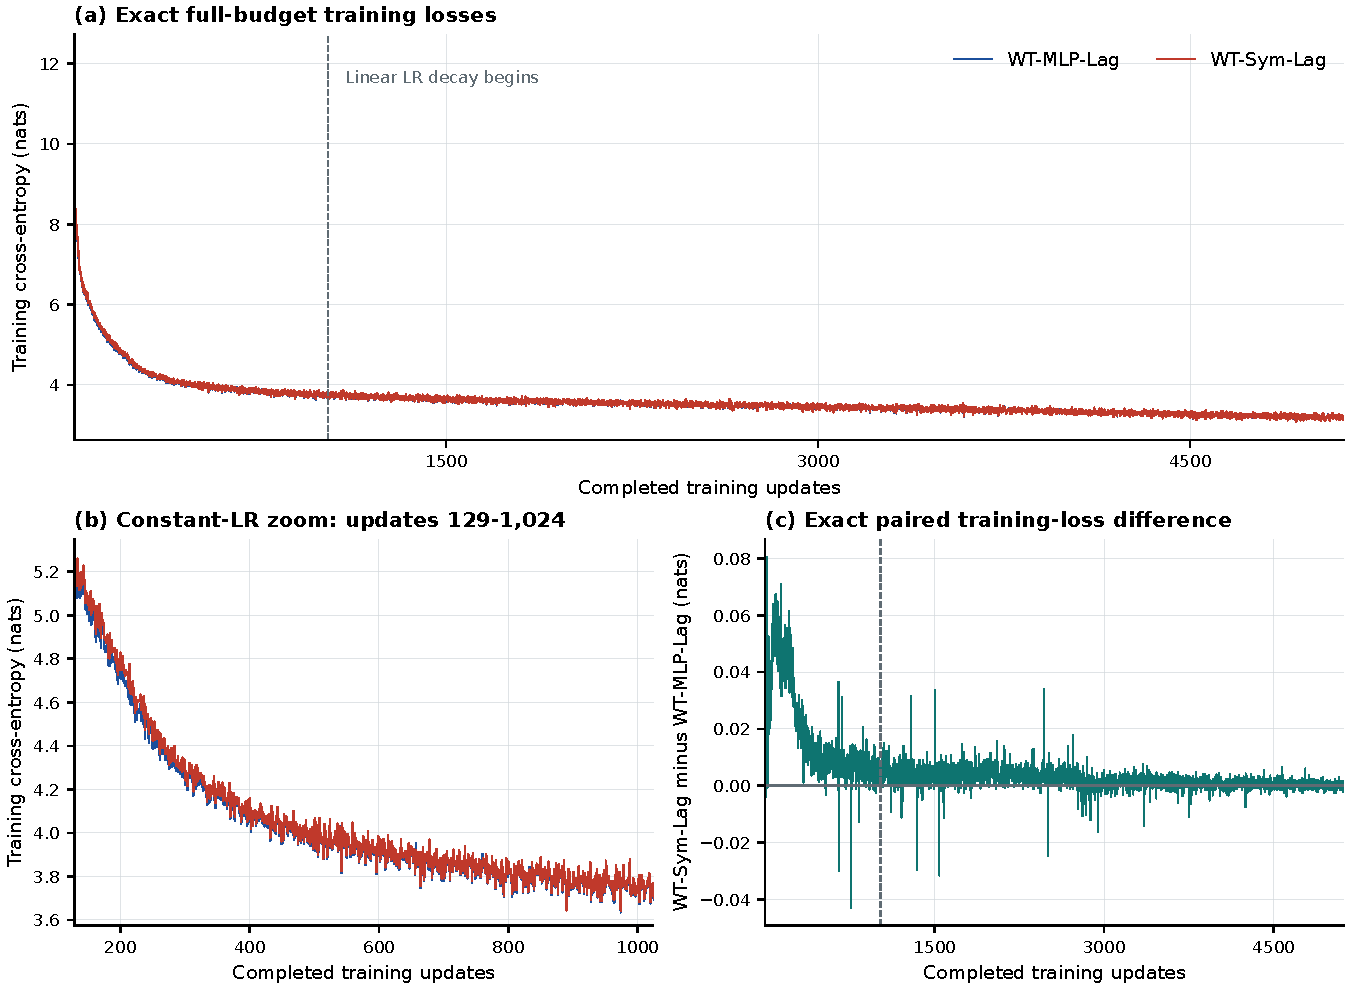
\includegraphics[width=\textwidth]{wt_lag_training.pdf}
\caption{Exact same-wave per-update training histories comparing asymmetric
\taxid{WT-MLP-Lag} against symmetric \taxid{WT-Sym-Lag} ($130\text{M}$ $1\times$,
seed~0, identical token order, \texttt{fast\_lag} runner; all $5{,}120$ logged
losses plotted with no smoothing, binning, or downsampling).
\textbf{(a)} Full $5{,}120$-update raw training loss per arm.
\textbf{(b)} Early constant-LR zoom over updates $129$--$1{,}024$.
\textbf{(c)} Exact paired difference (\taxid{WT-Sym-Lag} minus
\taxid{WT-MLP-Lag}; positive favors \taxid{WT-MLP-Lag}): diagonalizing
post-SwiGLU \texttt{in:down} incurs a $\symLagVsMlpLagWinOne{}$-nat mean
penalty during the constant-LR plateau (dashed vertical line at update
$1{,}024$) before contracting to $\symLagVsMlpLagWinFive{}$ during LR decay.}
\label{fig:q2-sym}
\end{figure}

\subsection{Q3: Learning-Rate Horizon Shift and Full-Budget LR Confirmation}
\label{sec:res-q3}

\paragraph{Short-schedule (320-step) learning-rate screening suffers severe horizon shift and invalidates transfer rankings.}
Before running full-budget tuning, we tested whether a 6\%-budget ($320$-update,
$0.17\text{B}$-token) seven-point sweep over $\eta \in [0.016, 0.128]$ could
predict full-budget optima (Figure~\ref{fig:q3}a). On the short schedule, every
arm shifted $2.8\times$--$4\times$ higher onto a flat plateau at $0.064$--$0.0905$,
where noise split two mathematically identical outer-diagonal arms
(\taxid{OD-Outer} versus \taxid{OD-Outer-F}) across $0.0905$ and $0.064$.
Carrying $0.064$ to the full 5{,}120-update budget \emph{degraded \taxid{MuonT}
itself by $\waveTwelveMuontSelDiff{}$ nats} relative to $0.0226$
($\waveTwelveMuontCfourDiff{}$ final C4), while pushing \taxid{OD-All} and
\taxid{OD-Outer} to $0.0905$ crossed the full-budget stability cliff
($+0.049$--$+0.050$ nats; Figure~\ref{fig:q3}b). Short-horizon screening is
therefore an invalid proxy; full-budget bracketing around $0.0226$ is mandatory.

\paragraph{Full-budget LR bracketing around $0.0226$ confirms that \taxid{WT-MLP-Lag} beats \taxid{MuonT} at every matched learning rate.}
Phase~1 of our \confTotalRuns{}-run \texttt{fast\_lag} confirmation campaign
bracketed $\{0.016, 0.0226, 0.032\}$ at full 5{,}120-update budget on seed~0
(Figure~\ref{fig:q3}c and Table~\ref{tab:confirmation}). Increasing $\eta$ to
$0.032$ degrades every arm ($+0.0044$ to $+0.0071$ final selection), while
$[0.016, 0.0226]$ forms the true interior optimum for all Toner-family arms
(whereas pushing plain \taxid{Muon} to $0.0226$ immediately hurts it by
$+0.0063$ nats). Crucially, \taxid{WT-MLP-Lag} beats \taxid{MuonT} on $11/11$
second-half evaluations at \emph{every} matched rate: by
$\confPOneZeroOneSixWtFinalSel{}$ final / $\confPOneZeroOneSixWtLateSel{}$
late-11 selection ($\confPOneZeroOneSixWtLateCfour{}$ late-11 C4,
$\confPOneZeroOneSixWtTrainHalf{} \pm \confPOneZeroOneSixWtTrainHalfSe{}$ across
$2{,}560$ second-half training updates) at $\eta = 0.016$, and by
$\confPOneZeroTwoTwoWtFinalSel{}$ final / $\confPOneZeroTwoTwoWtLateSel{}$
late-11 selection ($\confPOneZeroTwoTwoWtNetLateSel{}$ net of \texttt{fast\_lag}
\taxid{Null-WT}) at $\eta = 0.0226$.

\begin{figure}[t]
\centering
\resizebox{\textwidth}{!}{%
\begin{tikzpicture}
\begin{groupplot}[
  paperplot,
  group style={group size=3 by 1, horizontal sep=1.9cm},
  height=5.4cm,
]
\nextgroupplot[
  width=5.3cm,
  title={(a) 320-step screen ($0.17\text{B}$)},
  xlabel={Matrix learning rate $\eta$},
  ylabel={Final selection loss (nats)},
  xmode=log, log basis x=2,
  xmin=0.014, xmax=0.145, ymin=4.20, ymax=4.64,
  xtick={0.016,0.02262741696,0.032,0.04525483392,0.064,0.09050966784,0.128},
  xticklabels={.016,.023,.032,.045,.064,.091,.128},
  xticklabel style={font=\tiny, rotate=38, anchor=east},
  legend style={at={(0.97,0.96)}, anchor=north east, font=\tiny, inner sep=1.6pt},
  every axis plot/.append style={line width=0.95pt, mark size=1.6pt},
]
\fill[famNull!10] (axis cs:0.056,4.20) rectangle (axis cs:0.102,4.64);
\addplot[color=famRef, mark=oplus*] table[x=lr, y=muont] {figs/lr_sweep.dat};
\addlegendentry{\taxid{MuonT}}
\addplot[color=famOD, mark=diamond*] table[x=lr, y=inner_outer_leftdiag] {figs/lr_sweep.dat};
\addlegendentry{\taxid{OD-All}}
\addplot[color=famAbl, mark=triangle*] table[x=lr, y=outer_leftdiag] {figs/lr_sweep.dat};
\addlegendentry{\taxid{OD-Outer}}
\addplot[color=famWT, mark=square*] table[x=lr, y=outer_leftdiag_fused] {figs/lr_sweep.dat};
\addlegendentry{\taxid{OD-Outer-F}}

\nextgroupplot[
  width=5.35cm,
  unbounded coords=discard,
  title={(b) 5{,}120-step horizon shift},
  xlabel={Matrix learning rate $\eta$},
  ylabel={Late-11 selection loss (nats)},
  xmode=log, log basis x=2,
  xmin=0.014, xmax=0.120, ymin=3.345, ymax=3.585,
  scaled y ticks=false,
  ytick={3.36,3.40,3.44,3.48,3.52,3.56},
  yticklabel style={/pgf/number format/fixed, /pgf/number format/precision=2},
  xtick={0.016,0.02262741696,0.032,0.04525483392,0.064,0.09050966784},
  xticklabels={.016,.023,.032,.045,.064,.091},
  xticklabel style={font=\tiny, rotate=38, anchor=east},
  legend style={at={(0.03,0.97)}, anchor=north west, font=\tiny, inner sep=1.4pt},
  every axis plot/.append style={line width=0.95pt, mark size=1.8pt},
]
\fill[famWT!8] (axis cs:0.015,3.345) rectangle (axis cs:0.035,3.585);
\addplot[color=famRef, line width=1.1pt, mark=oplus*] table[x=lr, y=muont] {figs/lr_horizon.dat};
\addlegendentry{\taxid{MuonT}}
\addplot[only marks, color=famWT, mark=star, mark size=2.6pt] table[x=lr, y=wt_mlp] {figs/lr_horizon.dat};
\addlegendentry{\taxid{WT-MLP}}
\addplot[color=famOD, densely dotted, mark=diamond*] table[x=lr, y=od_all] {figs/lr_horizon.dat};
\addlegendentry{\taxid{OD-All}}
\draw[-Latex, famAbl, line width=0.9pt] (axis cs:0.064,3.377) -- (axis cs:0.064,3.471);
\node[font=\tiny, text=famAbl!95!black, align=left, anchor=west] at (axis cs:0.066,3.42) {$+0.1001$\\ over-step};

\nextgroupplot[
  width=5.35cm,
  title={(c) Full-budget Phase 1 bracket},
  xlabel={Matrix learning rate $\eta$},
  ylabel={Final selection loss (nats)},
  xmode=log, log basis x=2,
  xmin=0.0145, xmax=0.0355, ymin=3.228, ymax=3.255,
  scaled y ticks=false,
  ytick={3.230,3.235,3.240,3.245,3.250},
  yticklabel style={/pgf/number format/fixed, /pgf/number format/precision=3},
  xtick={0.016,0.02262741696,0.032},
  xticklabels={.016,.023,.032},
  legend style={at={(0.98,0.98)}, anchor=north east, font=\tiny, inner sep=1.6pt},
  every axis plot/.append style={line width=1.0pt, mark size=1.9pt},
]
\addplot[color=famRef!70, dash dot, mark=triangle*] table[x=lr, y=muon] {figs/conf_lr_grid.dat};
\addlegendentry{\taxid{Muon}}
\addplot[color=famRef, mark=oplus*] table[x=lr, y=muont] {figs/conf_lr_grid.dat};
\addlegendentry{\taxid{MuonT}}
\addplot[color=famOD, densely dashed, mark=diamond*] table[x=lr, y=od_all] {figs/conf_lr_grid.dat};
\addlegendentry{\taxid{OD-All}}
\addplot[color=famWT, line width=1.15pt, mark=star, mark size=2.6pt] table[x=lr, y=wt_mlp_lag] {figs/conf_lr_grid.dat};
\addlegendentry{\textbf{\taxid{WT-MLP-Lag}}}
\addplot[only marks, color=famNull, mark=square*, mark size=2.1pt] table[x=lr, y=null_wt] {figs/conf_lr_grid.dat};
\addlegendentry{\taxid{Null-WT}}
\end{groupplot}
\end{tikzpicture}%
}
\caption{Anatomy of learning-rate horizon shift versus full-budget tuning
confirmation ($130\text{M}$ $1\times$ Chinchilla, seed~0).
\textbf{(a)} On a 320-update ($6\%$-budget) screen, all arms shift $3\times$--$4\times$
higher onto a flat plateau ($0.064$--$0.0905$).
\textbf{(b)} Transferring $0.064$ to 5{,}120 updates degrades \taxid{MuonT} by
$+0.1001$ nats relative to $0.0226$ and pushes $0.0905$ past the stability cliff;
the true basin lies in $[0.016, 0.032]$ (shaded blue).
\textbf{(c)} Phase~1 full-budget \texttt{fast\_lag} bracket over
$\{0.016, 0.0226, 0.032\}$: \taxid{WT-MLP-Lag} beats \taxid{MuonT} cleanly at
every matched rate, while \texttt{fast\_lag} \taxid{Null-WT} sits directly on
\taxid{MuonT} ($\confNullFinalSelDelta{}$ final selection).}
\label{fig:q3}
\end{figure}

\subsection{Q4: Post-Selection Three-Seed Replication and 16-Domain Paloma Generalization}
\label{sec:res-q4}

\paragraph{\taxid{WT-MLP-Lag} replicates across three fresh post-selection seeds against tuned \taxid{MuonT} on both in-distribution and 16-domain Paloma metrics.}
Phase~2 evaluated all four core arms (\taxid{Muon}, \taxid{MuonT},
\taxid{OD-All}, \taxid{WT-MLP-Lag}) on three fresh paired post-selection seeds
(seeds~1, 2, 3) using Gate~1's pre-registered LRs (Table~\ref{tab:confirmation},
Phase~2). Because Gate~1 shifted \taxid{MuonT} down to $0.016$ while retaining
$0.0226$ for \taxid{OD-All} and \taxid{WT-MLP-Lag}, this test is strictly
conservative against \taxid{WT-MLP-Lag} (which also edged lower at $0.016$ on
seed~0). Even against tuned \taxid{MuonT} ($0.016$), \taxid{WT-MLP-Lag} wins
\textbf{$3/3$ fresh seeds} on every endpoint:
$\confPTwoWtSelDeltaMean{} \pm \confPTwoWtSelDeltaStd{}$ selection
($\confPTwoWtSelVsMuonMean{}$ versus \taxid{Muon}),
$\confPTwoWtCfourDeltaMean{} \pm \confPTwoWtCfourDeltaStd{}$ C4, and
$\confPTwoWtPalomaDeltaMean{} \pm \confPTwoWtPalomaDeltaStd{}$ macro mean across
all 16 Paloma domains ($\confPTwoWtPalomaVsMuonMean{}$ versus \taxid{Muon}) at
$+\confPTwoWtStepPct\%$ full-run median step time. Diagonal-only \taxid{OD-All}
achieves a much smaller margin ($\confPTwoOdSelDeltaMean{}$ selection,
$\confPTwoOdPalomaDeltaMean{}$ Paloma, $2/3$ seeds), corroborating the legacy
3-seed replication of \taxid{WT-MLP} ($-0.0061$, $-0.0042$, $-0.0040$ late-11
C4) while extending paired replication to all four core arms on the unified
\texttt{fast\_lag} runner.

\subsection{Q5: Persistence Under \texorpdfstring{$4\times$}{4x} Chinchilla Overtraining and \texorpdfstring{$520\text{M}$}{520M} Model Scaling}
\label{sec:res-q5}

\paragraph{Overtraining to $4\times$ Chinchilla ($80$ TPP, $10.74\text{B}$ tokens) preserves and widens \taxid{WT-MLP-Lag}'s matched-LR advantage.}
Scaling token horizon $4\times$ to $20{,}480$ updates with Marin's $4^{-0.3}$ LR
law initially propagated Gate~1's $41\%$ LR mismatch into Wave~3A
($\eta = 0.0149$ for \taxid{OD-All}/\taxid{WT-MLP-Lag} versus $0.0106$ for
\taxid{MuonT}), penalizing hot-LR \taxid{WT-MLP-Lag} by
$\confPThreeHotWtFinalSel{}$ final selection (Table~\ref{tab:confirmation}).
Resolving that confound in Wave~3B by matching $\eta = 0.0105561$
($\eta_{\text{aux}} = 0.0031668$) across all arms confirms that overtraining
does \emph{not} diminish output-side gains: \taxid{WT-MLP-Lag} beats
\taxid{MuonT} on $11/11$ second-half evaluations ($\confPThreeWtLateSel{}$
late-11, $\confPThreeWtFinalSel{}$ final selection; $\confPThreeWtLateCfour{}$
late-11, $\confPThreeWtFinalCfour{}$ final C4; $\confPThreeWtVsMuonFinalSel{}$
final selection versus \taxid{Muon}), delivers
$\confPThreeWtTrainHalf{} \pm \confPThreeWtTrainHalfSe{}$ across $10{,}240$
second-half training updates ($|t| > 200$), and wins
\textbf{$\confPThreeWtPalomaWins{}/16$ Paloma domains}
($\confPThreeWtPalomaDelta{}$ macro mean) at $+\confPThreeWtStepPct\%$ step
time. Diagonal-only \taxid{OD-All} retains roughly half the gain
($\confPThreeOdFinalSel{}$ final selection, $\confPThreeOdPalomaDelta{}$ Paloma,
$\confPThreeOdPalomaWins{}/16$ domains).

\paragraph{Scaling $4\times$ in non-embedding parameters to $520\text{M}$ ($799.6\text{M}$ total) preserves \taxid{WT-MLP-Lag}'s gain while diagonal-only \taxid{OD-All} loses its edge.}
Evaluating all four core arms at $520\text{M}$ ($d=1024$, $d_{\text{mlp}}=4096$,
$L=32$, $10.74\text{B}$ tokens, $1\text{M}$ batch) under Toner's pinned matched
LR ($\eta = 0.0226274$, $\eta_{\text{aux}} = 0.0024$; reproducing upstream C4
references closely at $\confPFourMuonFinalCfourAbs{}$ for \taxid{Muon} and
$\confPFourMuontFinalCfourAbs{}$ for \taxid{MuonT}) cleanly separates
asymmetric width-thresholding from pure diagonal output normalization
(Table~\ref{tab:confirmation} and Figure~\ref{fig:q5}). \taxid{WT-MLP-Lag}
beats \taxid{MuonT} on $11/11$ second-half evaluations ($21/21$ post-step-1
evaluations) by $\confPFourWtLateSel{}$ late-11 ($\confPFourWtFinalSel{}$ final)
selection, $\confPFourWtLateCfour{}$ late-11 ($\confPFourWtFinalCfour{}$ final)
C4, $\confPFourWtTrainHalf{} \pm \confPFourWtTrainHalfSe{}$ across $5{,}120$
second-half updates ($|t| = 136$), and $\confPFourWtPalomaDelta{}$ across all 16
Paloma domains (winning \textbf{$\confPFourWtPalomaWins{}/16$ domains};
$\confPFourWtVsMuonFinalSel{}$ versus \taxid{Muon}) at $+\confPFourWtStepPct\%$
step time ($\confPFourWtGib{}$ versus $\confPFourMuontGib{}$\,GiB peak). In
contrast, diagonal-only \taxid{OD-All} fades slightly behind \taxid{MuonT}
($\confPFourOdFinalSel{}$ final / $\confPFourOdLateSel{}$ late-11 selection,
$\confPFourOdPalomaDelta{}$ Paloma, $\confPFourOdPalomaWins{}/16$ domains),
demonstrating that dense residual-stream output whitening ($d=1024$) is
essential at larger width while pre-SwiGLU width-$4096$ outputs remain safely
diagonal.

\paragraph{Multi-horizon step averaging confirms that every matched-LR delta is resolved well above evaluation noise.}
Across every matched-LR regime in Table~\ref{tab:confirmation}, the 11-point
second-half held-out mean ($\approx 8.65\text{M}$ selection tokens,
between-checkpoint SE $0.00025$--$0.00038$ nats, $8\times$--$18\times$ below
\taxid{WT-MLP-Lag}'s gain) agrees closely with both the last-5 evaluation mean
and final step, while autocorrelation-inflated paired training SEs over
$2{,}560$--$10{,}240$ second-half updates reach $0.00002$--$0.00004$ nats
($\rho_1 \in [0.04, 0.12]$, $|t| > 100$).

\begin{table}[t]
\centering
\caption{Master confirmation and scaling summary across \confTotalRuns{}
\texttt{fast\_lag} runs and \confPalomaCount{} 16-domain Paloma evaluations
(negative deltas favor the candidate; every delta is paired within regime
against the listed \taxid{MuonT} reference row, which reports absolute losses).
\textbf{Late-11 $\Delta$Sel} averages all 11 second-half evaluations
($\text{step} > T/2$) with per-checkpoint win counts; \textbf{2nd-Half
$\Delta$Train$\pm$SE} is the lag-1 autocorrelation-inflated paired training
difference over the full second half ($2{,}560$, $10{,}240$, or $5{,}120$
updates); \textbf{16-Dom Paloma $\Delta$} reports macro-mean deltas with domain
(or seed) win counts; \textbf{Step\% / GiB} uses full-run post-warmup median
step times across all $5{,}120$--$20{,}480$ updates. Mid-decay averages are
omitted in Phase~2 because Gate~1 paired \taxid{MuonT} at $0.016$ against
\taxid{OD-All}/\taxid{WT-MLP-Lag} at $0.0226$.}
\label{tab:confirmation}
\scriptsize\setlength{\tabcolsep}{3.1pt}
\resizebox{\textwidth}{!}{% Generated by scripts/integrate_confirmation_campaign.py. Do not edit.
\begin{tabular}{@{}lccccccc@{}}
\toprule
Regime / Arm & $\eta$ & Final $\Delta$Sel & Late-11 $\Delta$Sel (Wins) & Final $\Delta$C4 & 2nd-Half $\Delta$Train$\pm$SE & 16-Dom Paloma $\Delta$ & Step\% / GiB \\
\midrule
\multicolumn{8}{@{}l}{\textcolor{famRef}{\pagesfsb Phase 1: $130\text{M}$ $1\times$ Chinchilla ($20$ TPP, $2.68\text{B}$ tok, Seed 0) --- Full-Budget LR Bracket \& \texttt{fast\_lag} Null}} \\
\taxid{MuonT} (ref @ $.016$) & $.016$ & $3.2342$ & $3.3591$ (ref) & $3.4511$ & $0$ ($2{,}560$ upd.) & --- & $0.0\%$ / 20.5 \\
\taxid{Muon} (ref @ $.016$) & $.016$ & $+0.0119$ & $+0.0234$ (0/11) & $+0.0107$ & $+0.0238\pm0.00070$ & --- & $-2.2\%$ / 19.0 \\
\rowcolor{pagepanel} \textbf{\taxid{WT-MLP-Lag} (matched)} & $.016$ & $\mathbf{-0.0038}$ & $\mathbf{-0.0047}$ (11/11) & $\mathbf{-0.0039}$ & $-0.0038\pm0.00004$ & --- & $+3.8\%$ / 21.6 \\
\taxid{MuonT} (ref @ $.0226$) & $.0226$ & $3.2354$ & $3.3763$ (ref) & $3.4511$ & $0$ ($2{,}560$ upd.) & --- & $0.0\%$ / 20.5 \\
\taxid{Null-WT} (\texttt{fast\_lag}) & $.0226$ & $-0.0003$ & $-0.0008$ (9/11) & $-0.0006$ & $-0.0007\pm0.00004$ & --- & $+11.5\%$ / 21.5 \\
\taxid{OD-All} (matched) & $.0226$ & $-0.0021$ & $-0.0039$ (11/11) & $-0.0022$ & $-0.0026\pm0.00004$ & --- & $+1.3\%$ / 20.5 \\
\rowcolor{pagepanel} \textbf{\taxid{WT-MLP-Lag} (matched)} & $.0226$ & $\mathbf{-0.0043}$ & $\mathbf{-0.0047}$ (11/11) & $\mathbf{-0.0021}$ & $-0.0014\pm0.00005$ & --- & $+4.9\%$ / 21.6 \\
\addlinespace[2.5pt]
\multicolumn{8}{@{}l}{\textcolor{famWT}{\pagesfsb Phase 2: $130\text{M}$ $1\times$ Chinchilla ($20$ TPP) --- Fresh Post-Selection 3-Seed Paired Replication (Seeds 1, 2, 3; Gate-1 LRs)}} \\
\taxid{MuonT} (3-seed mean) & $.016$ & $3.1916$ & --- & $3.4523$ & --- & $3.4049$ (ref) & $0.0\%$ / 20.5 \\
\taxid{Muon} (3-seed paired) & $.016$ & $+0.0119$ (0/3) & --- & $+0.0118$ (0/3) & --- & $+0.0115$ (0/3) & $-1.9\%$ / 19.0 \\
\taxid{OD-All} (3-seed paired) & $.0226$ & $-0.0005\pm0.0005$ (3/3) & \emph{(hotter LR)} & $-0.0029$ (3/3) & \emph{(hotter LR)} & $-0.0009$ (2/3) & $+1.7\%$ / 20.5 \\
\rowcolor{pagepanel} \textbf{\taxid{WT-MLP-Lag}} (3-seed) & $.0226$ & $\mathbf{-0.0034}\pm0.0014$ (3/3) & \emph{(hotter LR)} & $\mathbf{-0.0035}$ (3/3) & \emph{(hotter LR)} & $\mathbf{-0.0040}$ (3/3) & $+5.1\%$ / 21.6 \\
\addlinespace[2.5pt]
\multicolumn{8}{@{}l}{\textcolor{famOD}{\pagesfsb Phase 3A/3B: $130\text{M}$ $4\times$ Chinchilla ($80$ TPP, $10.74\text{B}$ tok, $20{,}480$ upd., Seed 0) --- Overtraining Horizon}} \\
\taxid{MuonT} (3A ref) & $.0106$ & $3.0675$ & $3.2013$ (ref) & $3.2886$ & $0$ ($10{,}240$ upd.) & $3.2368$ (ref) & $0.0\%$ / 20.5 \\
\taxid{Muon} (3A) & $.0106$ & $+0.0103$ & $+0.0223$ (0/11) & $+0.0103$ & $+0.0224\pm0.00027$ & $+0.0111$ (1/16) & $-1.8\%$ / 19.0 \\
\taxid{OD-All} (3B matched) & $.0106$ & $-0.0019$ & $-0.0016$ (10/11) & $-0.0026$ & $-0.0023\pm0.00002$ & $-0.0026$ (15/16) & $+1.9\%$ / 20.5 \\
\rowcolor{pagepanel} \textbf{\taxid{WT-MLP-Lag} (3B matched)} & $.0106$ & $\mathbf{-0.0040}$ & $\mathbf{-0.0045}$ (11/11) & $\mathbf{-0.0038}$ & $-0.0041\pm0.00002$ & $\mathbf{-0.0057}$ (16/16) & $+5.5\%$ / 21.6 \\
\taxid{WT-MLP-Lag} (3A $+41\%$ LR) & $.0149$ & $+0.0020$ & $+0.0190$ (0/11) & $+0.0014$ & $+0.0202\pm0.00047$ & $+0.0036$ (5/16) & $+5.7\%$ / 21.6 \\
\addlinespace[2.5pt]
\multicolumn{8}{@{}l}{\textcolor{famDT}{\pagesfsb Phase 4: $520\text{M}$ $1\times$ Chinchilla ($20$ TPP, $10.74\text{B}$ tok, $1\text{M}$ batch, $10{,}240$ upd., Seed 0) --- Pinned Matched LR}} \\
\taxid{MuonT} (4A ref) & $.0226$ & $2.8463$ & $2.9839$ (ref) & $3.0704$ & $0$ ($5{,}120$ upd.) & $3.0256$ (ref) & $0.0\%$ / 27.4 \\
\taxid{Muon} (4A pinned) & $.016$ & $+0.0065$ & $+0.0019$ (3/11) & $+0.0065$ & $+0.0006\pm0.00009$ & $+0.0035$ (1/16) & $-4.1\%$ / 20.5 \\
\taxid{OD-All} (4A matched) & $.0226$ & $+0.0006$ & $+0.0006$ (2/11) & $+0.0004$ & $-0.0005\pm0.00002$ & $+0.0005$ (6/16) & $+2.6\%$ / 27.5 \\
\rowcolor{pagepanel} \textbf{\taxid{WT-MLP-Lag} (4A matched)} & $.0226$ & $\mathbf{-0.0028}$ & $\mathbf{-0.0030}$ (11/11) & $\mathbf{-0.0022}$ & $-0.0024\pm0.00002$ & $\mathbf{-0.0054}$ (15/16) & $+10.5\%$ / 31.6 \\
\bottomrule
\end{tabular}
}
\end{table}

\begin{figure}[t]
\centering
\resizebox{\textwidth}{!}{%
\begin{tikzpicture}
\begin{groupplot}[
  paperplot,
  group style={group size=2 by 1, horizontal sep=2.2cm},
  height=5.3cm,
]
\nextgroupplot[
  width=7.8cm,
  title={(a) Matched-LR $\Delta$ selection trajectories across scale \& horizon},
  xlabel={Normalized training progress ($t / T$)},
  ylabel={$\Delta$ Selection vs.\ \taxid{MuonT} (nats)},
  xmin=0.04, xmax=1.02, ymin=-0.0092, ymax=0.0022,
  scaled y ticks=false,
  ytick={-0.008,-0.006,-0.004,-0.002,0,0.002},
  yticklabel style={/pgf/number format/fixed, /pgf/number format/precision=3},
  legend columns=2,
  legend style={at={(0.98,0.03)}, anchor=south east, font=\tiny, inner sep=1.6pt},
  every axis plot/.append style={line width=1.0pt, mark size=1.5pt},
]
\fill[famWT!5] (axis cs:0.50,-0.0092) rectangle (axis cs:1.02,0);
\draw[pagemuted!80, dashed, line width=0.55pt] (axis cs:0.04,0) -- (axis cs:1.02,0);
\draw[pagemuted!60, densely dotted, line width=0.55pt] (axis cs:0.50,-0.0092) -- (axis cs:0.50,0.0022);
\addplot[color=famWT, line width=1.1pt, mark=o] table[x=progress, y=wt_130_1x] {figs/conf_traj_delta.dat};
\addlegendentry{\taxid{WT} $130\text{M}$ $1\times$ (.016)}
\addplot[color=famDT, line width=1.1pt, mark=square*] table[x=progress, y=wt_130_4x] {figs/conf_traj_delta.dat};
\addlegendentry{\taxid{WT} $130\text{M}$ $4\times$ (.0106)}
\addplot[color=famAbl, line width=1.15pt, mark=star, mark size=2.3pt] table[x=progress, y=wt_520_1x] {figs/conf_traj_delta.dat};
\addlegendentry{\taxid{WT} $520\text{M}$ $1\times$ (.0226)}
\addplot[color=famOD, densely dashed, mark=diamond] table[x=progress, y=od_130_4x] {figs/conf_traj_delta.dat};
\addlegendentry{\taxid{OD} $130\text{M}$ $4\times$ (.0106)}
\addplot[color=famNull, densely dotted, line width=1.1pt, mark=triangle] table[x=progress, y=od_520_1x] {figs/conf_traj_delta.dat};
\addlegendentry{\taxid{OD} $520\text{M}$ $1\times$ (.0226)}

\nextgroupplot[
  width=7.1cm,
  ybar=2.0pt, bar width=8.0pt,
  title={(b) Post-hoc 16-domain Paloma macro-mean $\Delta$},
  ylabel={$\Delta$ Paloma macro vs.\ \taxid{MuonT} (nats)},
  xmin=-0.55, xmax=2.55, ymin=-0.0072, ymax=0.0135,
  xtick={0,1,2},
  xticklabels={
    {\shortstack{$130\text{M}$ $1\times$\\ {\tiny(3 fresh seeds)}}},
    {\shortstack{$130\text{M}$ $4\times$\\ {\tiny(80 TPP matched)}}},
    {\shortstack{$520\text{M}$ $1\times$\\ {\tiny(20 TPP matched)}}}
  },
  xticklabel style={font=\tiny},
  scaled y ticks=false,
  ytick={-0.006,-0.003,0,0.003,0.006,0.009,0.012},
  yticklabel style={/pgf/number format/fixed, /pgf/number format/precision=3},
  legend style={at={(0.98,0.98)}, anchor=north east, font=\tiny, inner sep=1.8pt},
]
\draw[pagemuted!80, line width=0.55pt] (axis cs:-0.55,0) -- (axis cs:2.55,0);
\addplot[fill=famRef!60, draw=famRef] table[x=idx, y=muon] {figs/conf_paloma.dat};
\addlegendentry{\taxid{Muon}}
\addplot[fill=famOD!75, draw=famOD] table[x=idx, y=od_all] {figs/conf_paloma.dat};
\addlegendentry{\taxid{OD-All}}
\addplot[fill=famWT!85, draw=famWT] table[x=idx, y=wt_mlp_lag] {figs/conf_paloma.dat};
\addlegendentry{\textbf{\taxid{WT-MLP-Lag}}}
\end{groupplot}
\end{tikzpicture}%
}
\caption{Matched-LR scaling trajectories and external 16-domain Paloma
generalization across horizons and model scale.
\textbf{(a)} Paired $\Delta$ selection loss across all 21 post-step-1
evaluations (shaded region indicates the 11-point second-half reporting window,
$t/T > 0.5$): \taxid{WT-MLP-Lag} stays strictly negative on $11/11$ second-half
evaluations at $130\text{M}$ $1\times$, $130\text{M}$ $4\times$, and
$520\text{M}$ $1\times$, while diagonal-only \taxid{OD-All} drifts above zero at
$520\text{M}$.
\textbf{(b)} Post-hoc 16-domain Paloma macro-mean $\Delta$ against
\taxid{MuonT}: \taxid{WT-MLP-Lag} improves every regime ($3/3$ fresh seeds at
$130\text{M}$ $1\times$, $\confPThreeWtPalomaWins{}/16$ domains at $130\text{M}$
$4\times$, and $\confPFourWtPalomaWins{}/16$ domains at $520\text{M}$ $1\times$).}
\label{fig:q5}
\end{figure}

\subsection{Q6: Paired Comparison Against Contemporary Two-Sided Muon Designs}
\label{sec:res-q6}

\paragraph{Under common isotropic decay ($\lambda=0.1$) on fresh seeds~1 and~2, \taxid{WT-MLP} leads \texttt{muon\_control}, Mousse, and GO-MUON.}
To contextualize asymmetric width-thresholding against contemporary two-sided
spectral optimizers, we executed a separate 30-trial paired campaign comparing
vanilla \taxid{Muon} (\texttt{muon\_control}) and \taxid{WT-MLP} against
\textbf{Mousse} \citep{zhang2026mousse} (gradient-Gram moments with $\alpha=1/8$
tempering) and \textbf{GO-MUON} \citep{che2026gomuon} (quarter-power
$\alpha=1/4$ activation/cotangent roots with global Frobenius grafting),
separating common-setting formula controls from paper-recipe adapters under
shared isotropic $\lambda = 0.1$ decay (Table~\ref{tab:related}). At the
Stage-1-selected rate ($\eta = 0.032$) across fresh seeds~1 and~2,
\taxid{WT-MLP} leads all six arms with $\relWtFinalSelDeltaMean{}$ mean final
selection ($\relWtLateSelDeltaMean{}$ late-11, $\relWtFinalCfourDeltaMean{}$
final C4), confirming that its benefit does not depend on input-shaped decay.
\taxid{Mousse-Ctrl} closely tracks \texttt{muon\_control}
($\relMousseCtrlFinalSelDeltaMean{}$), \taxid{Mousse-Paper} finishes slightly
behind ($\relMoussePaperFinalSelDeltaMean{}$), and both GO-MUON variants finish
behind ($\relGoCtrlFinalSelDeltaMean{}$ and $\relGoPaperFinalSelDeltaMean{}$).

\paragraph{GO-MUON's early surge and constant-LR reversal reflect quarter-power Frobenius grafting and upper-boundary LR censoring rather than implementation error.}
Exact per-update paired training curves (Figure~\ref{fig:related}) rule out
coding bugs: \texttt{go\_muon\_control} and \texttt{go\_muon\_paper} use
disjoint statistics and polar routines yet track each other within
$\relGoPaperMinusCtrlFinalSel{}$ nats. Both surge to a
$\relGoCtrlEarlyMinSOne{}$-to-$\relGoCtrlEarlyMinSTwo{}$-nat early lead near
updates $\relGoCtrlEarlyMinStepSOne{}$--$\relGoCtrlEarlyMinStepSTwo{}$ while
spectra are near-isotropic, then cross behind \taxid{Muon} near updates
$\relGoCtrlCrossStepSOne{}$--$\relGoCtrlCrossStepSTwo{}$ --- more than $800$
updates before LR decay begins --- as global Frobenius grafting on $\alpha=1/4$
outer powers attenuates active high-variance directions. Because all six arms
hit the $0.032$ upper grid ceiling and GO-MUON's deficit shrank monotonically
with $\eta$ (Figure~\ref{fig:related}c), these runs diagnose an interaction
between quarter-power grafting, LR censoring, and isotropic decay rather than
claiming inferiority of a fully tuned GO-MUON.

\begin{table}[t]
\centering
\caption{Paired comparison against Mousse \citep{zhang2026mousse} and GO-MUON
\citep{che2026gomuon} under common isotropic matrix weight decay
($\lambda = 0.1$, $130\text{M}$ $1\times$ Chinchilla; negative deltas favor the
candidate relative to \texttt{muon\_control}, whose row reports absolute
losses). \textbf{Short $\Delta$Sel} shows the 320-update seed-0 screen across
$\{0.016, 0.0226, 0.032\}$ (all arms hit the $0.032$ ceiling); full-budget
columns average fresh paired seeds~1 and~2 at frozen $\eta = 0.032$, reporting
final selection, 11-point late selection, final C4, Window~1$\to$Window~5
paired training means, total wall-clock seconds, and peak Rank-0 GiB.}
\label{tab:related}
\scriptsize\setlength{\tabcolsep}{3.4pt}
\resizebox{\textwidth}{!}{% Generated by scripts/plot_related_baselines.py. Do not edit.
\begin{tabular}{@{}llcccccccc@{}}
\toprule
Arm & Moments (in, out) & Short $\Delta$Sel ($.016/.023/.032$) & S1 / S2 $\Delta$Sel & Mean $\Delta$Sel & Late-11 $\Delta$Sel & Final $\Delta$C4 & $\Delta$Train (W1$\to$W5) & Total s (\%) & GiB \\
\midrule
\multicolumn{10}{@{}l}{\textcolor{famRef}{\pagesfsb I.\ Shared Controls (Deduplicated Across Both Panels; Baseline Row Reports Absolute Losses)}} \\
\taxid{Muon} {\scriptsize(\texttt{muon\_ctrl})} & None ($\mathcal{N}_{10}$) & $4.614 / 4.528 / 4.461$ & $3.2204 / 3.1944$ & $0.0000$ & $0.0000$ & $3.4841$ & $0.000 \to 0.000$ & $6,102$ (ref) & $18.5$ \\
\rowcolor{pagepanel} \textbf{\taxid{WT-MLP}} {\scriptsize(\texttt{mlpdiag})} & Act/Cot $(\tfrac{1}{2},\tfrac{1}{8})$ & $-0.035 / -0.091 / -0.126$ & $-0.0118 / -0.0080$ & $\mathbf{-0.0099}$ & $-0.0071$ & $-0.0099$ & $-0.098 \to -0.006$ & $7,391$ ($+21\%$) & $22.6$ \\
\addlinespace[2.5pt]
\multicolumn{10}{@{}l}{\textcolor{famOD}{\pagesfsb II.\ Common-Setting Formula Controls (EMA $\beta=0.938$, Ridge $10^{-3}$, Refresh $4$, 10-Step BF16 NS)}} \\
\taxid{Mousse-Ctrl} & Grad Gram $(\tfrac{1}{8},\tfrac{1}{8})$ & $+0.042 / +0.005 / -0.033$ & $-0.0010 / -0.0010$ & $-0.0010$ & $+0.0012$ & $-0.0019$ & $-0.074 \to +0.001$ & $8,098$ ($+33\%$) & $19.0$ \\
\taxid{GO-MUON-Ctrl} & Act/Cot $(\tfrac{1}{4},\tfrac{1}{4})$ & $+0.085 / +0.059 / +0.049$ & $+0.0336 / +0.0283$ & $+0.0310$ & $+0.0382$ & $+0.0294$ & $-0.013 \to +0.035$ & $9,277$ ($+52\%$) & $21.8$ \\
\addlinespace[2.5pt]
\multicolumn{10}{@{}l}{\textcolor{famAbl}{\pagesfsb III.\ Paper-Recipe Adapters (Author Numerics/Refresh; Common Model, Data, Schedule, Isotropic $\lambda=0.1$)}} \\
\taxid{Mousse-Paper} & Grad Gram $(\tfrac{1}{8},\tfrac{1}{8})$ & $+0.004 / -0.073 / -0.134$ & $+0.0022 / +0.0034$ & $+0.0028$ & $+0.0049$ & $+0.0032$ & $-0.083 \to +0.006$ & $6,697$ ($+10\%$) & $19.0$ \\
\taxid{GO-MUON-Paper} & Act/Cot $(\tfrac{1}{4},\tfrac{1}{4})$ & $+0.114 / +0.091 / +0.086$ & $+0.0353 / +0.0288$ & $+0.0321$ & $+0.0397$ & $+0.0305$ & $+0.008 \to +0.036$ & $11,854$ ($+94\%$) & $21.8$ \\
\bottomrule
\end{tabular}
}
\end{table}

\begin{figure}[t]
\centering
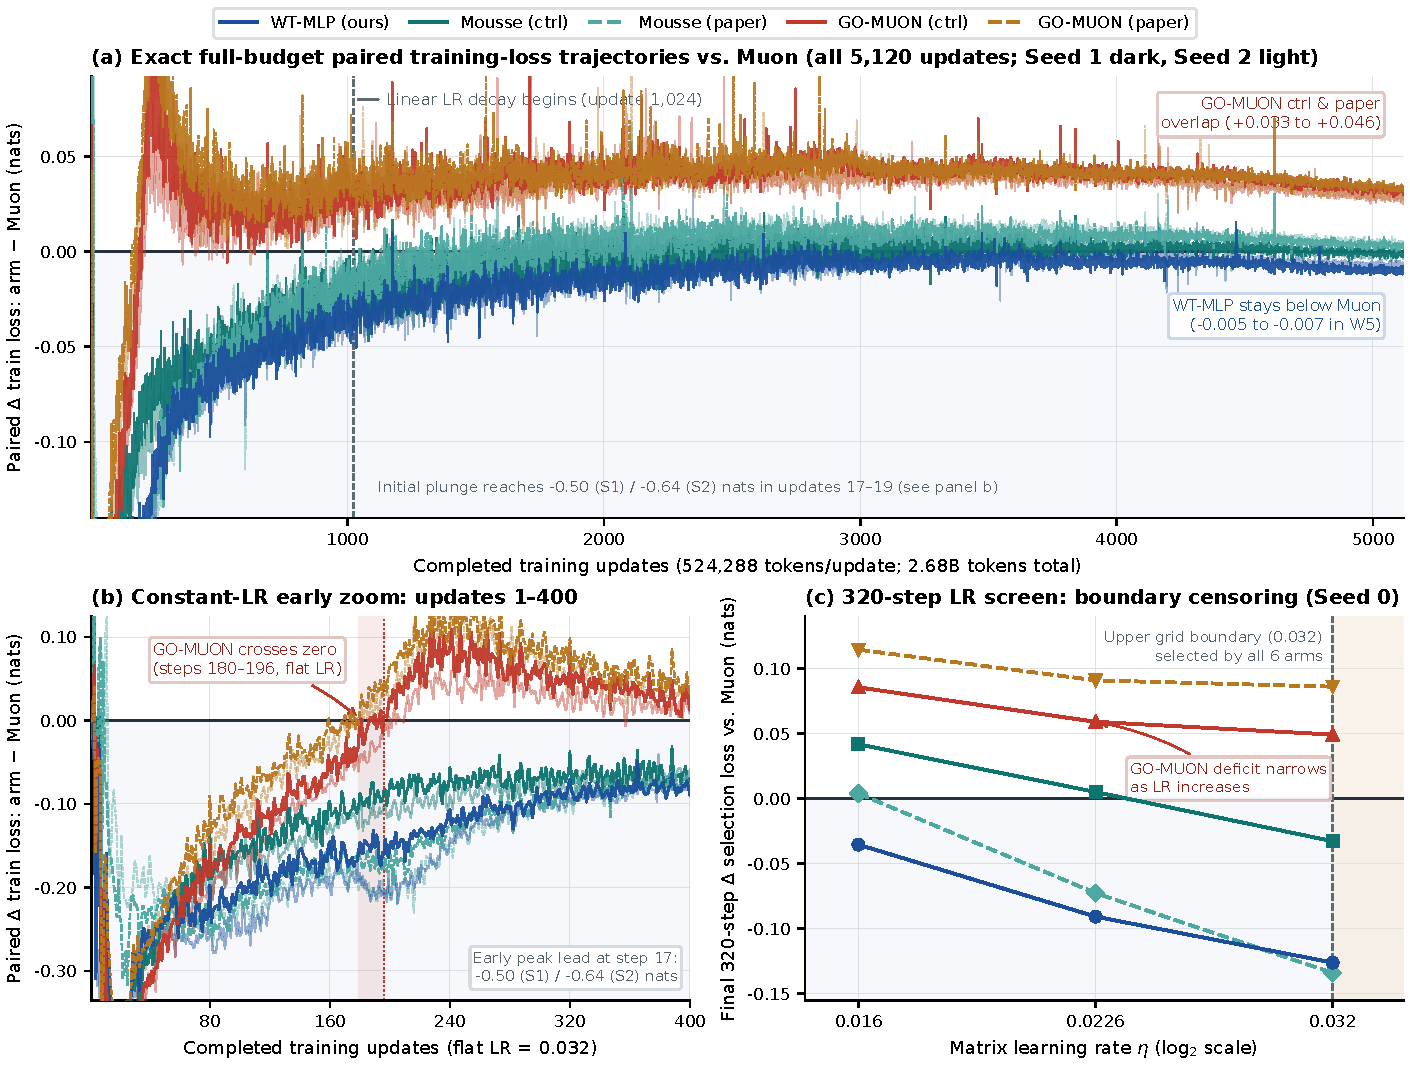
\includegraphics[width=\textwidth]{related_baselines_training.pdf}
\caption{Exact per-update training dynamics and LR-boundary censoring across the
paired related-baseline campaign ($5{,}120$ updates per arm at frozen
$\eta=0.032$ on fresh seeds~1 and~2 under isotropic $\lambda=0.1$ decay; no
smoothing or downsampling).
\textbf{(a)} Paired training-loss difference versus seed-matched
\texttt{muon\_control} (negative favors candidate; Seed~1 darker, Seed~2
lighter).
\textbf{(b)} Early-training zoom (updates $1$--$400$, inside the flat-LR
plateau) showing GO-MUON's initial surge and constant-LR crossover near update
$200$.
\textbf{(c)} 320-update seed-0 LR screen showing monotonic improvement into the
$0.032$ upper grid boundary.}
\label{fig:related}
\end{figure}

\subsection{Q7: Eight-GPU Systems Overhead and Wall-Clock Time-to-Target}
\label{sec:res-q7}

\paragraph{Eliminating barriers, fallback stalls, and SIMT products reduces \texttt{fast\_lag} steady-step overhead to $+3.8\%$--$+5.8\%$ at $130\text{M}$ and $+10.5\%$ at $520\text{M}$.}
On the legacy synchronous research runner, even diagonal-only \taxid{OD-All}
incurred $+10.4\%$ steady-step overhead while \taxid{WT-MLP} paid $+21.9\%$ and
legacy \taxid{WT-MLP-Lag} paid $+18.0\%$. On uncontended eight-A100 nodes,
\texttt{fast\_lag} cuts full-run steady-step overhead over \taxid{MuonT} by more
than $3\times$: to $+\sysExecSymLagVsMuontPct\%$ on \taxid{WT-Sym-Lag}
($\sysExecSymLagGib$\,GiB) and $+\confPTwoWtStepPct\%$--$+\sysExecMlpLagVsMuontPct\%$
on \taxid{WT-MLP-Lag} ($\sysExecMlpLagGib$\,GiB; $+\confPThreeWtStepPct\%$ over
$20{,}480$ steps at $130\text{M}$ $4\times$). At $520\text{M}$ ($d=1024$,
microbatch~1 on 40\,GB A100s), \taxid{WT-MLP-Lag}'s overhead rises modestly to
$+\confPFourWtStepPct\%$ ($\confPFourWtGib{}$ versus $\confPFourMuontGib{}$\,GiB),
remaining well within single-node 40\,GB VRAM.

\paragraph{Bringing step overhead below the $\sysTokenSavingPct\%$ token-saving threshold converts legacy wall-clock deficits into a launch-anchored win at $\text{C4}\le 3.52$.}
At $130\text{M}$ $1\times$, every width-thresholded arm reaches
$\text{C4}\le 3.52$ at update $4{,}501$ ($2.36\text{B}$ tokens) versus update
$4{,}751$ ($2.49\text{B}$ tokens) for \taxid{MuonT} and \taxid{Muon} --- a
$\sysTokenSavingPct\%$ token saving ($250$ updates; Table~\ref{tab:systems-v2}).
Because legacy runners paid $18\%$--$22\%$ per-step overhead, they crossed
targets $600$--$1{,}100$\,s \emph{later} than \taxid{MuonT}. Once
\texttt{fast\_lag} drops overhead to $+\sysExecSymLagVsMuontPct\%$,
\taxid{WT-Sym-Lag} crosses $\text{C4}\le 3.52$ in
$\sysCrossSymLagThreeFiveTwoS$\,s --- ahead of same-wave \taxid{MuonT}
($\sysCrossMuontSymThreeFiveTwoS$\,s), Wave-0 \taxid{MuonT}
($\sysCrossMuontWaveZeroThreeFiveTwoS$\,s), and vanilla \taxid{Muon}
($\sysCrossMuonWaveZeroThreeFiveTwoS$\,s) in launch-anchored wall-clock time,
while \texttt{fast\_lag} \taxid{WT-MLP-Lag} saves $600$\,s over legacy Wave~4
and edges Wave-0 \taxid{MuonT} ($\sysCrossMlpLagFastThreeFiveTwoS$\,s) while
retaining the strongest held-out mixture quality.

\begin{table}[t]
\centering
\caption{Launch-anchored eight-A100 wall-clock time-to-target crossings on
Paloma \texttt{c4\_en} ($130\text{M}$ $1\times$ Chinchilla, seed~0,
$2.68\text{B}$ tokens). Elapsed times include compilation, training,
evaluation, and checkpointing from job launch; step indices mark the first
logged evaluation meeting each C4 threshold. \taxid{Muon} fails to reach
$\text{C4}\le 3.46$ within the $5{,}120$-update budget (censored at
$\waveZeroMuonCfourFinalAbs{}$).}
\label{tab:systems-v2}
\footnotesize\setlength{\tabcolsep}{5.0pt}
\resizebox{\textwidth}{!}{% Generated by scripts/analyze_systems.py. Do not edit.
\begin{tabular}{@{}lrrrrr@{}}
\toprule
Arm (wave / runner) & $\text{C4}\le 3.59$ & $\text{C4}\le 3.52$ & $\text{C4}\le 3.46$ & Final C4 & Total E2E \\
\midrule
\taxid{Muon} {\scriptsize(\texttt{wave0})} & $4{,}880.0$\,s {\scriptsize(step 4{,}251)} & $5{,}467.0$\,s {\scriptsize(step 4{,}751)} & \textcolor{famAbl}{\textbf{Censored}} {\scriptsize($3.4618$)} & $3.4618$ & $5{,}889.7$\,s \\
\taxid{MuonT} {\scriptsize(\texttt{wave0})} & $4{,}721.3$\,s {\scriptsize(step 4{,}001)} & $5{,}566.3$\,s {\scriptsize(step 4{,}751)} & $5{,}848.2$\,s {\scriptsize(step 5{,}001)} & $3.4527$ & $5{,}984.6$\,s \\
\taxid{MuonT} {\scriptsize(\texttt{wave\_sym\_fastlag})} & $4{,}619.6$\,s {\scriptsize(step 4{,}001)} & $5{,}468.4$\,s {\scriptsize(step 4{,}751)} & $5{,}754.4$\,s {\scriptsize(step 5{,}001)} & $3.4511$ & $5{,}891.3$\,s \\
\rowcolor{pagepanel} \textbf{\taxid{WT-Sym-Lag}} {\scriptsize(\texttt{fast\_lag})} & $4{,}869.6$\,s {\scriptsize(step 4{,}001)} & $\mathbf{5{,}458.9}$\,\textbf{s} {\scriptsize(step 4{,}501)} & $6{,}040.3$\,s {\scriptsize(step 5{,}001)} & $\mathbf{3.4482}$ & $6{,}179.3$\,s \\
\rowcolor{pagepanel} \textbf{\taxid{WT-MLP-Lag}} {\scriptsize(\texttt{fast\_lag})} & $4{,}966.4$\,s {\scriptsize(step 4{,}001)} & $5{,}564.6$\,s {\scriptsize(step 4{,}501)} & $6{,}157.2$\,s {\scriptsize(step 5{,}001)} & $3.4491$ & $6{,}300.3$\,s \\
\taxid{WT-Sym} {\scriptsize(no-lag, $\tau=0$)} & $5{,}187.7$\,s {\scriptsize(step 4{,}001)} & $5{,}822.6$\,s {\scriptsize(step 4{,}501)} & $6{,}446.1$\,s {\scriptsize(step 5{,}001)} & $\mathbf{3.4482}$ & $6{,}593.9$\,s \\
\taxid{WT-MLP-Lag} {\scriptsize(legacy Wave 4)} & $5{,}500.6$\,s {\scriptsize(step 4{,}001)} & $6{,}164.4$\,s {\scriptsize(step 4{,}501)} & $6{,}824.2$\,s {\scriptsize(step 5{,}001)} & $\mathbf{3.4480}$ & $6{,}985.7$\,s \\
\taxid{WT-MLP} {\scriptsize(legacy Wave 2)} & $5{,}624.4$\,s {\scriptsize(step 4{,}001)} & $6{,}309.1$\,s {\scriptsize(step 4{,}501)} & $6{,}981.7$\,s {\scriptsize(step 5{,}001)} & $\mathbf{3.4464}$ & $7{,}142.0$\,s \\
\bottomrule
\end{tabular}
}
\end{table}

\FloatBarrier

\bibliographystyle{plainnat}
\bibliography{refs}

\end{document}
